\iftoggle{DEBUG}{
\chapter{Adquisición Fonética en Dinámica Cortical}
}{
\chapter{Phonetic Acquisition in Cortical Dynamics}
}

\label{ch:phonetics}

\iftoggle{DEBUG}{
\section{Introducción}


Se sabe que los humanos tienen la capacidad de discriminar fonemas y otras unidades lingüísticas clasificándolas sin importar la variabilidad evidenciada por diferentes hablantes con distintos tonos de voz y prosodia. De hecho, dichas capacidades de clasificación se trasladan a ambientes ruidosos y reverberantes.

Aunque dicha competencia  podría ser atribuida en parte a la información proveniente de activaciones corticales originadas en fenómenos cognitivos de orden superior \cite{PMID:17451657}, por ejemplo, fenómenos de dimensión gramatical y semántica  \cite{OBLESER2011713,10.1093/cercor/bhp128} presentes en el lenguaje humano--más allá de las características fonéticas de la señal del habla--se  ha demostrado que una gran variedad de animales entrenados también tienen la capacidad de discriminar pares de fonemas categóricamente y de generalizar frente a situaciones novedosas~\cite{kuhl_1975, kuhl_1983, kluender_1998, pons_2006, hienz_1996, dent_1997, lotto_1997}. Por ejemplo, activaciones corticales en hurones revelan la existencia de una especialización espectro-temporal en la \gls{a1} con la capacidad de sostener la discriminación de varios fonemas del Inglés Americano \cite{mesgarani_2008}, aún cuando el estímulo fue distorsionado por ruido aditivo y reverberación \cite{mesgarani_2014A}.

Pero aún más notable es como algunas tareas de adquisición temprana de lenguaje--de extremada complejidad--como la segmentación de palabras desde el flujo del habla, pueden ser realizadas por infantes de 8 meses de edad basándose simplemente en las relaciones estadísticas entre sonidos adyacentes en el habla \cite{Saffran1996StatisticalLB}. Después de sólo dos minutos de exposición a un flujo de habla continuo generado por un sintetizador de voz, los infantes mostraron adquisición y discriminación exitosa. Es más, en la fase de entrenamiento, no se presentó información alguna acerca de los límites de las palabras más allá de de la estructura estadística de las reglas fonotácticas inmersas en el estímulo. Los infantes tampoco recibieron ningún tipo de supervisión externa o refuerzo que pudiera haber guiado o impulsado la tarea de adquisición fonética, la cual fue completamente incidental.

Dicha invarianza adquirida incidentalmente en la percepción fonética de los mamíferos se debe basar necesariamente en características neurofisiológicas y anatómicas de la corteza de los mismos. Las características que estimamos potencialmente relevantes son agrupadas en el presente trabajo a los fines de plantear nuestras hipótesis computacionales.
}{
\section{Introduction}

It is well known that human beings can reliably discriminate phonemes as well as other linguistic units by categorizing them, despite considerable variability across different speakers with different pitches and prosody. Furthermore, this ability extends to noisy and reverberant environments.

Although such proficiency could in part be attributed to top-down information \cite{PMID:17451657} originated in the grammatical and semantic \cite{OBLESER2011713,10.1093/cercor/bhp128} dimensions present in human language--beyond the phonetic features in the speech signal--trained animals are also able to discriminate phoneme pairs categorically and to generalize in novel situations~\cite{kuhl_1975, kuhl_1983, kluender_1998, pons_2006, hienz_1996, dent_1997, lotto_1997}. For instance, cortical activations in naive ferrets revealed the existence of spectro-temporal tuning in \gls{a1} with the capacity of supporting discrimination of many American English phonemes \cite{mesgarani_2008}, even when stimuli were distorted by additive noise and reverberation \cite{mesgarani_2014A}.

It is even more remarkable that an extremely complex task of early language acquisition as is the segmentation of words from fluent speech, is fulfilled by 8-month-old infants based simply on the statistical relationships between neighboring speech sounds \cite{Saffran1996StatisticalLB}. With only 2 minutes of exposure to a continuous speech stream generated by a speech synthesizer, infants showed succesful phonetic acquisition and discrimination. Furthermore, in the training phase there was no acoustic information about word boundaries beyond the statistical structure in the phonotactic rules immerse in the stimuli, and the subjects received no external associative supervision or reinforcement which could have guided or boosted the phonetic acquisition task, which was entirely incidental.

This incidentally acquired invariance in phonetic perception found in mammals must be grounded necessarily in anatomical and neurophysiological characterisitcs of the mammalian cortex. The features we foresee as potentially relevant are brought together in order to pose our computational hypotheses.
}















\iftoggle{DEBUG}{
\subsection{Características anatómicas y neurofisiológicas de la corteza de mamíferos}

Linden y Schreiner \cite{linden_2003} resaltaron que aunque los circuitos corticales auditivos tienen algunas características únicas que requieren especial atención, sus similitudes con otras regiones sensoriales--como la corteza visual y la somatosensorial--son categóricas.
Primero, a nivel sensorial, el mapeo de frecuencia unidimensional coclear podría ser análogo a los mapeos espaciales bidimensionales que se encuentran en la retina o en la superficie del cuerpo.
Segundo, los mapas tonotópicos en el sistema auditivo podrían ser análogos a las organizaciones retinotópicas o somatotópicas halladas en las cortezas visual y somatosensorial respectivamente.
Las curvas de respuesta en frecuencia en el sistema auditivo podría corresponderse con los límites en las regiones espaciales en los campos receptivos visual y somatosensorial.
Cierta correspondencia se podría trazar entre la tasa de modulación de amplitud en el sistema auditivo y la sensibilidad de parpadeo en el sistema visual, o la sensibilidad a la bibración de bigotes en el sistema somatosensorial.
Finalmente, los campos auditivos receptivos adaptados para barrido de frecuencia, podrían ser análogos a la sensibilidad de movimiento visual y somatosensorial.

Estudios de gran impacto han mostrado que la \gls{a1} comparte características estructurales comunes con otras cortezas sensoriales.
De hecho, cuando las entradas retinales se rutean dentro del tálamo auditivo, células corticales auditivas desarrollan propiedades de respuestas tales como la selectividad direccional, la preferencia de orientación y los campos receptivos simples y complejos \cite{Sur1437, doi:10.1002/(SICI)1096-9861(19981026)400:3<417::AID-CNE10>3.0.CO;2-O, Roe1992VisualPR}.
Los mapas retinotópicos, en términos de adaptación de orientación con conectividad lateral entre dominios de orientación, emergen en las capas superficiales de la corteza auditiva recableada \cite{Roe818, Sharma2000InductionOV}.

Estos datos sugieren la existencia de una circuitería neuronal con capacidades de procesamiento similares para diferentes modalidades. Consecuentemente, agrupamos características anatómicas y fisiológicas encontradas en  el tejido cortical en general que intuimos relevantes para la invarianza y generalización en la percepción fonética. 

Una de las principales características neuroanatómicas de la corteza cerebral en mamíferos es que las células corticales están agrupadas espacialmente en dominios definidos por areas en campos receptivos comunes. Dichos alineamientos son llamados \glsfirst{cc_pl}~\cite{mountcastle_1955, mountcastle_1957, hubel_1962, hubel_1968}. Dentro de las \glspl{cc}, las mini-columnas corticales son agrupamientos de células que responden a estímulos con características similares (Fig. \ref{fig:Biological}). Adicionalmente, las columnas corticales están conectadas dentro de y entre diferentes regiones del tejido cortical formando una red de conectividad compleja pero organizada~\cite{mountcastle_1997}.

\begin{figure}[h!]
    \centering
    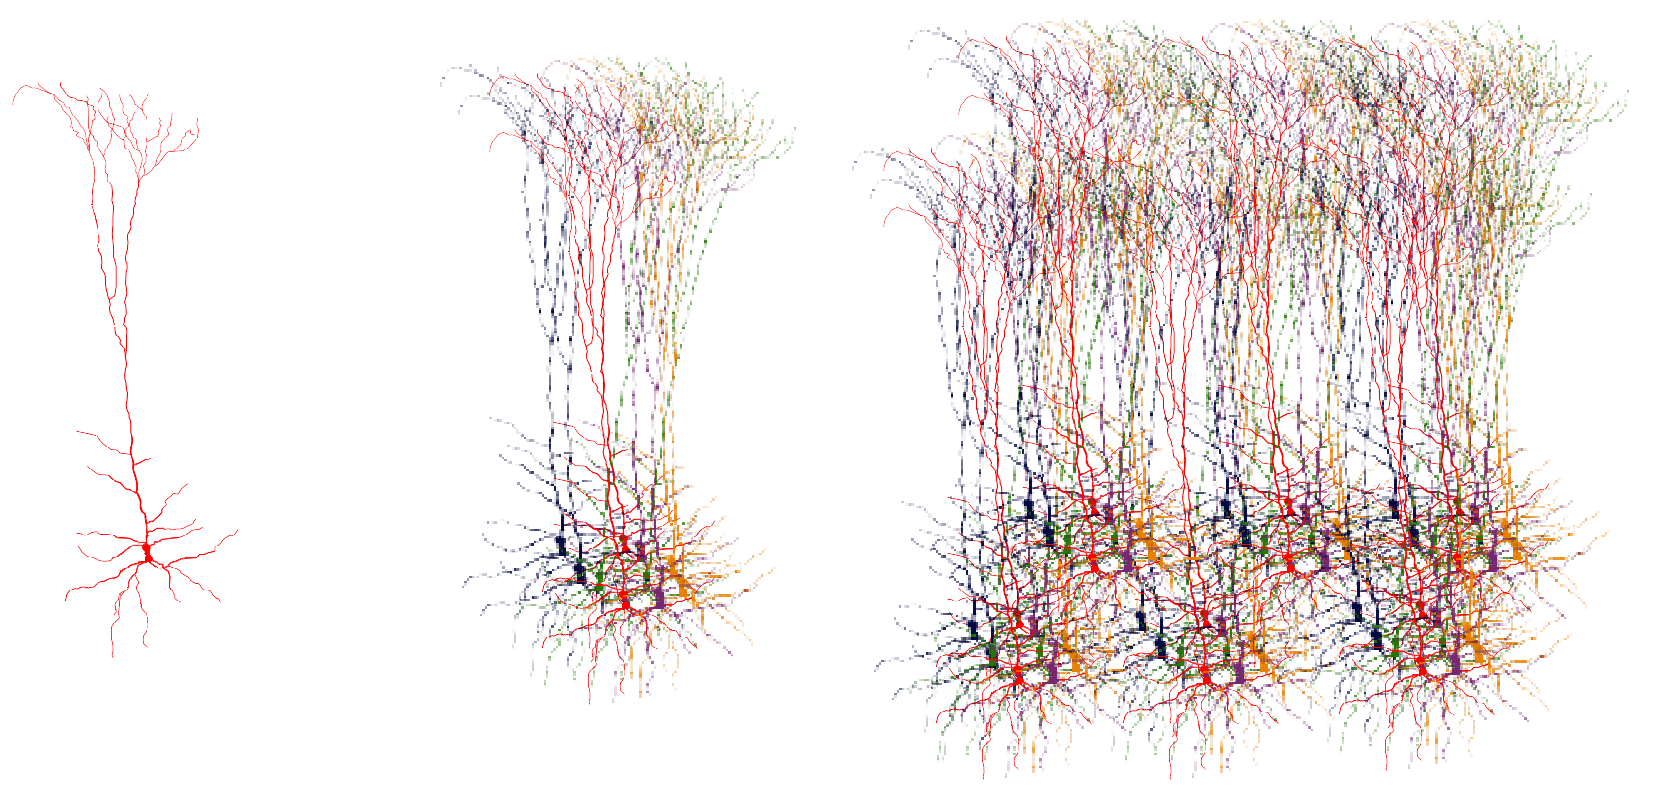
\includegraphics[width=1.0\textwidth]{Biological.png}
    \caption{Organización del tejido cortical. Izquierda: Célula piramidal. La neurona exitatoria más común en el tejido cortical.
	    Centro: Mini-columna cortical. Un aglomeramiento de células que responden a estímulos de características similares.
	    Derecha: Columna Cortical. Un grupo de mini-columnas con un campo receptivo en común.
	    Adaptada de (Fabuio, Own work, CC BY 4.0, \url{https://commons.wikimedia.org/w/index.php?curid=60707501)}}
    \label{fig:Biological}
\end{figure}

Una de las propiedades funcionales halladas en muchas de estas redes es la adaptación a los estímulos contextuales \cite{KRAUSE201436,doi:10.1167/16.13.1}. Se piensa que tal mecanismo sirve para aumentar la eficiencia en la codificación de la información sensorial. Por ejemplo, una reducción en las respuestas a sonidos frecuentes por medio de redes inhibitorias podría aumentar la sensibilidad cortical ante ruidos raros que podrían representar eventos inesperados~\cite{Natan2015ComplementaryCO,nachum_2003,Javitt11962}.

Finalmente, hallazgos recientes en neurociencia muestran que la corteza de los mamíferos procesa la información por medio de \gls{sdr_pl}~\cite{barth_2012}. Este mecanismo ofrece discriminación robusta y de baja tasa de error de la representación de los estímulos minimizando la activación neuronal durante la tarea en relación a los recursos neuronales disponibles para la representación~\cite{ahmad_2016}. En Hawkins et al. \cite{hawkins_2016} sostienen que uno de los mecanismos que podría estar involucrado en las redes corticales para formar \gls{sdr_pl} implica una depolarización extendida del núcleo de la célula como resultado de activaciones \gls{nmda} de ramas dendríticas independientes producidas por la excitación de cierto número de sinapsis distales~\cite{antic_2010, major_2013}.

En el presente trabajo las características neurofisiológicas y anatómicas de la corteza de los mamíferos arriba mencionadas son agrupadas como potencialmente relevantes a la hora de obtener invarianza fonética en la corteza auditiva de los mismos. Nuestro modelo de neurona piramidal disocia las ramas dendríticas distales de las próximas (Fig.~\ref{fig:PyramidalCell}). Las dendritas próximas actúan como un conjunto homogéneo recibiendo solo información aferente. La información en las dendritas próximas determinan un conjunto de unidades neuronales en una \gls{cc}, las cuales podrían ser activadas dependiendo de las activaciones previas en \glspl{cc} vecinas así como en la misma \gls{cc}.

\begin{figure}[h!]
    \centering
    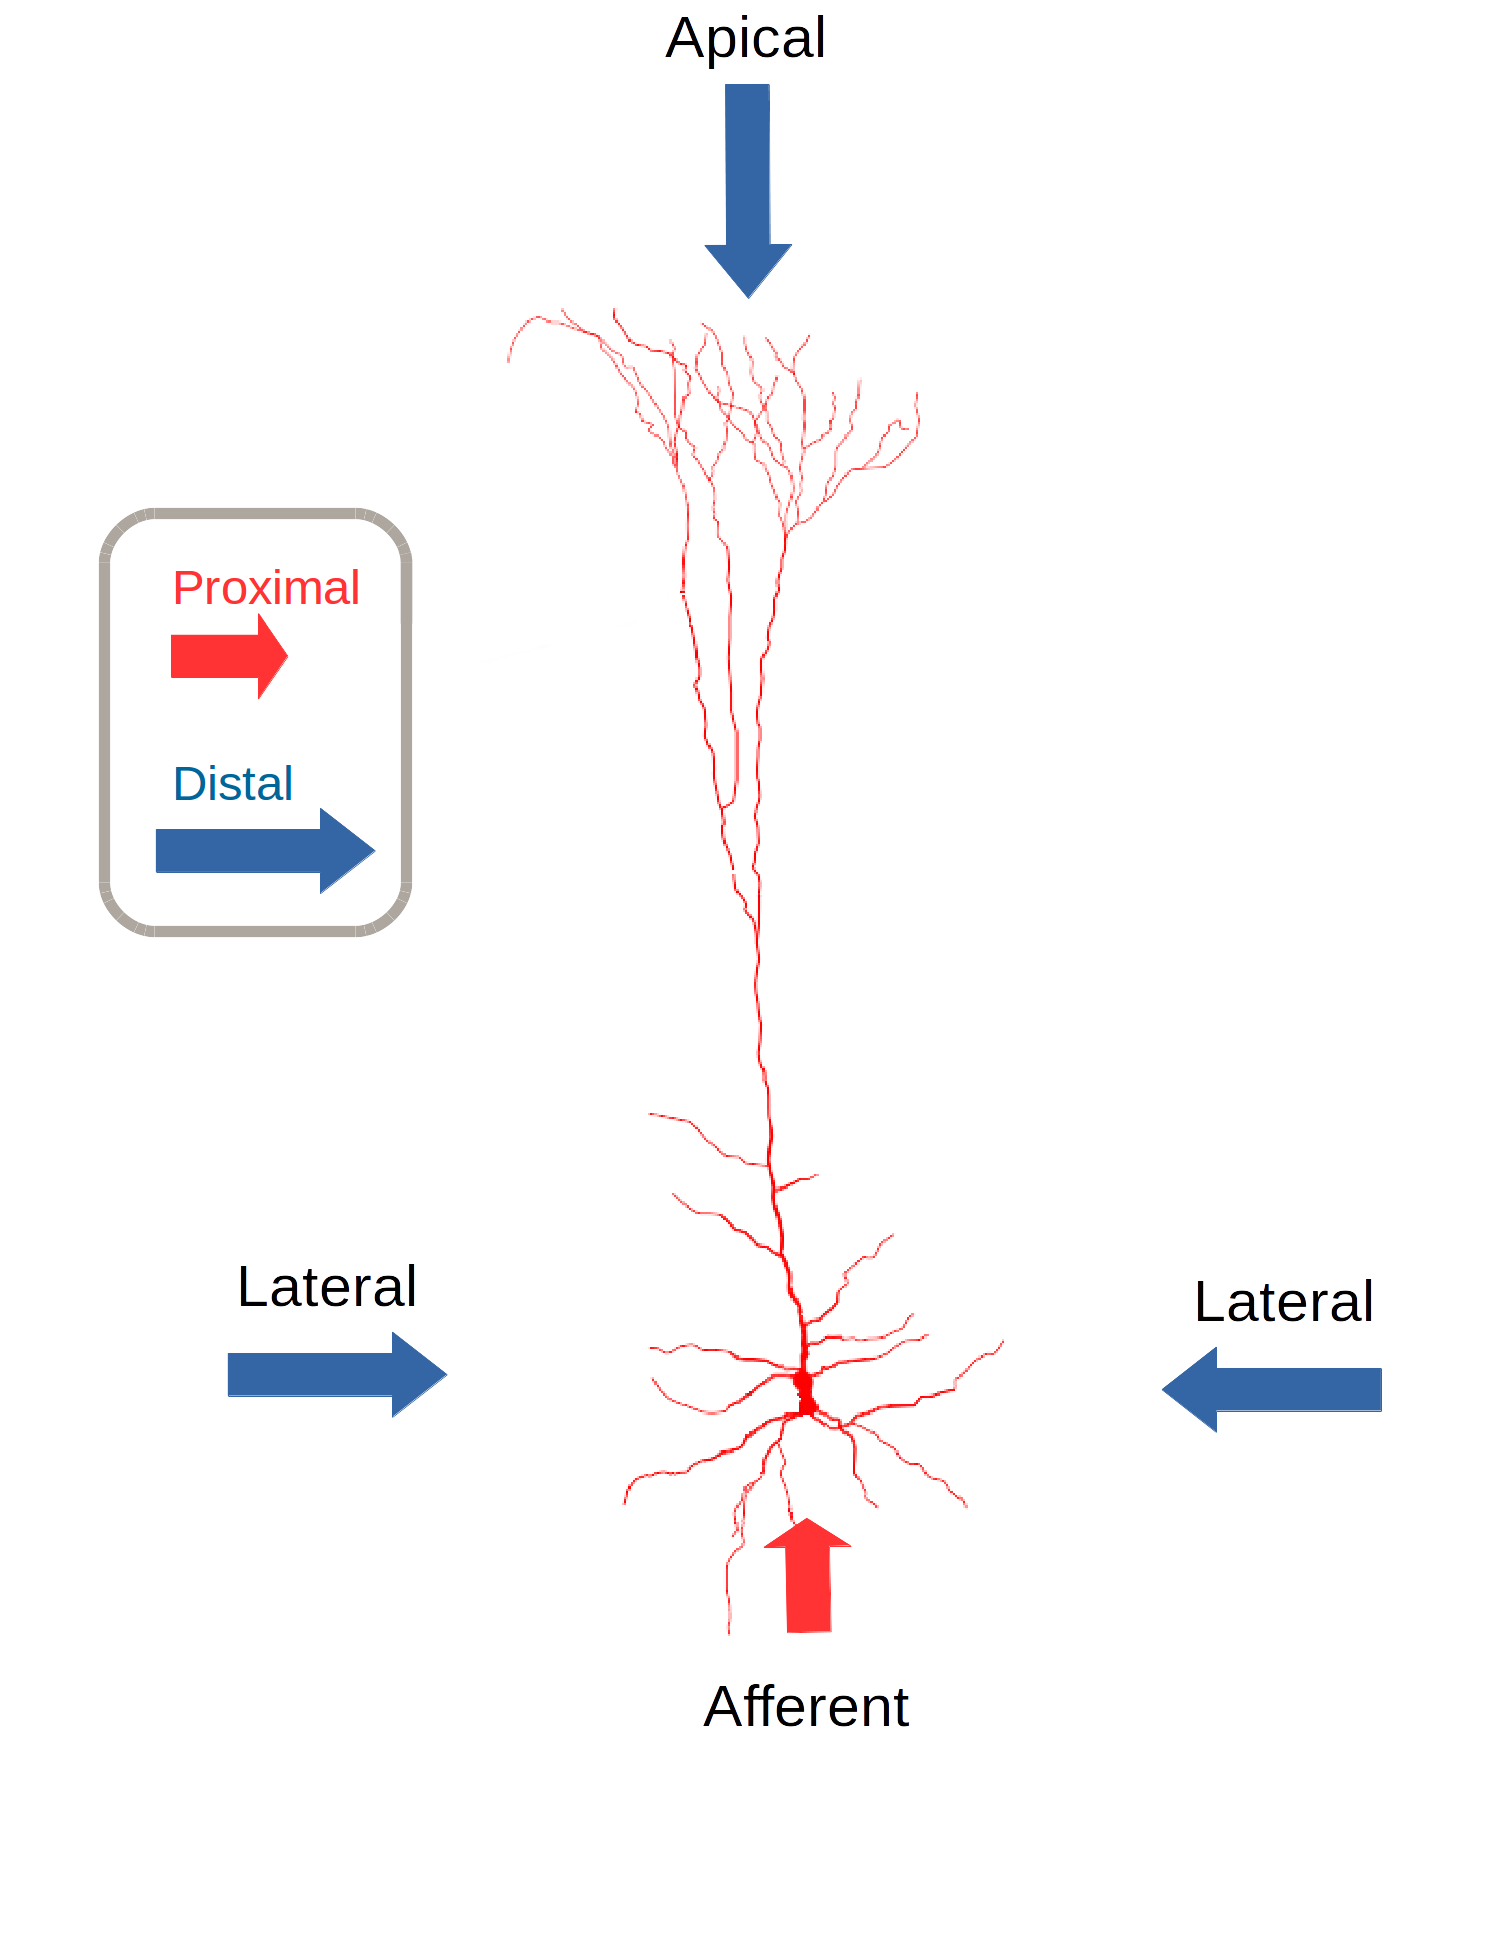
\includegraphics[width=0.5\textwidth]{PyramidalCell.png}
    \caption{Perfil de conectividad de una unidad neuronal piramidal en la \glsfirst{el}.
	    Las conexiones próximas se forman solo por conexiones aferentes desde el \glsfirst{mrstsa}
	    mientras que las conexiones diltales se forman por conexiones laterales y apicales desde columnas vecinas y
	    desde columnas en otras capas corticales arriba respectivamente.
	    La \gls{el} es la etapa más importante en nuestro modelo computacional mientras que el \gls{mrstsa} pre-procesa los corpus de audio para alimentar a la \gls{el}.
	    Adaptada de (Fabuio - Own work, CC BY 4.0, \url{https://commons.wikimedia.org/w/index.php?curid=60707501)}}
    \label{fig:PyramidalCell}
\end{figure}

Las dendritas distales reciben solo información lateral y apical actuando como detectores independientes. La información dendrítica distal pre-activa unidades neuronales poniéndolas en un estado predictivo para recibir información aferente futura.

Testeamos esos principios prestando especial atención a la dinámica temporal del habla, la cual juega el rol más importante en los contrastes lingüísticos~\cite{doi:10.1098/rstb.1992.0070}. Utilizamos un modelo computational no supervisado y biológicamente inspirado ya que nuestro objetivo es imitar la adquisición fonética incidental en infantes en cuya circunstancias, ninguna supervisión podría ser justificada. Nuestro modelo produce niveles de exactitud en clasificación fonética similares a aquellos surgidos desde enfoques profundos de clasificación de patrones. Por lo tanto, proponemos una ruta alternativa para abordar discriminación fonética basada en la observación de propiedades estructurales y funcionales presentes en la corteza de los mamíferos. 
}{
\subsection{Anatomical and neurophysiological characteristics of mammalian cortex}

Linden and Schreiner \cite{linden_2003}
highlighted that although auditory cortical circuits have some unique characteristics which require special attention,
their similarities with other sensory regions--such as visual or somatosensory cortex--turn out to be categorical.
First, at the sensory level, the cochlear one-dimensional frequency map could be analogous to the two-dimensional spatial maps which are found
in the retina or body surface.
Second, the tonotopic maps found in the auditory system could be analogous to the retinotopic and somatotopic organization found in visual and somatosensory cortices,
respectively.
Frequency tuning curves in the auditory system could correspond to inhibition of spatial surrounding boundaries in visual and somatosensory receptive fields.
A correspondence could be drawn between amplitude modulation rate in the auditory system and flicker sensitivity in the visual system, or
whisker vibration sensitivity in the somatosensory system.
Finally, auditory receptive fields tuned for frequency-sweep, could be analogous to visual and somatosensory motion sensitivity.

Compelling physiological studies have shown that \glsfirst{a1} shares common structural
characteristics with other sensory cortices.
Furthermore,  when retinal inputs are routed into the auditory thalamus, auditory cortical cells develop visual response properties such as direction selectivity, orientation preference and complex and simple receptive fields
\cite{Sur1437, doi:10.1002/(SICI)1096-9861(19981026)400:3<417::AID-CNE10>3.0.CO;2-O, Roe1992VisualPR}.
Retinotopic maps, in terms of orientation tuning with lateral connectivity between orientation domains, emerge in superficial layers of the rewired
auditory cortex \cite{Roe818, Sharma2000InductionOV}.

The above data suggest the existence of neuronal circuitry with similar processing capabilities for different modalities. Consequently, we gather physiological and anatomical characteristics found in cortical tissue in general which we foresee as relevant for phonetic perception invariance and generalization.

One of the main neuroanatomical features of brain cortex in mammals is that cortical cells are spacially arranged into domains defined by common receptive field locations. These alignments are called \glspl{cc}~\cite{mountcastle_1955, mountcastle_1957, hubel_1962, hubel_1968}. Within \glspl{cc}, cortical mini-columns are clusters of cells which respond to stimuli with similar characteristics (Fig. \ref{fig:Biological}). In addition, cortical columns are connected within and between different regions in cortical tissue forming a complex and yet organized connectivity network~\cite{mountcastle_1997}. 

\begin{figure}[h!]
    \centering
    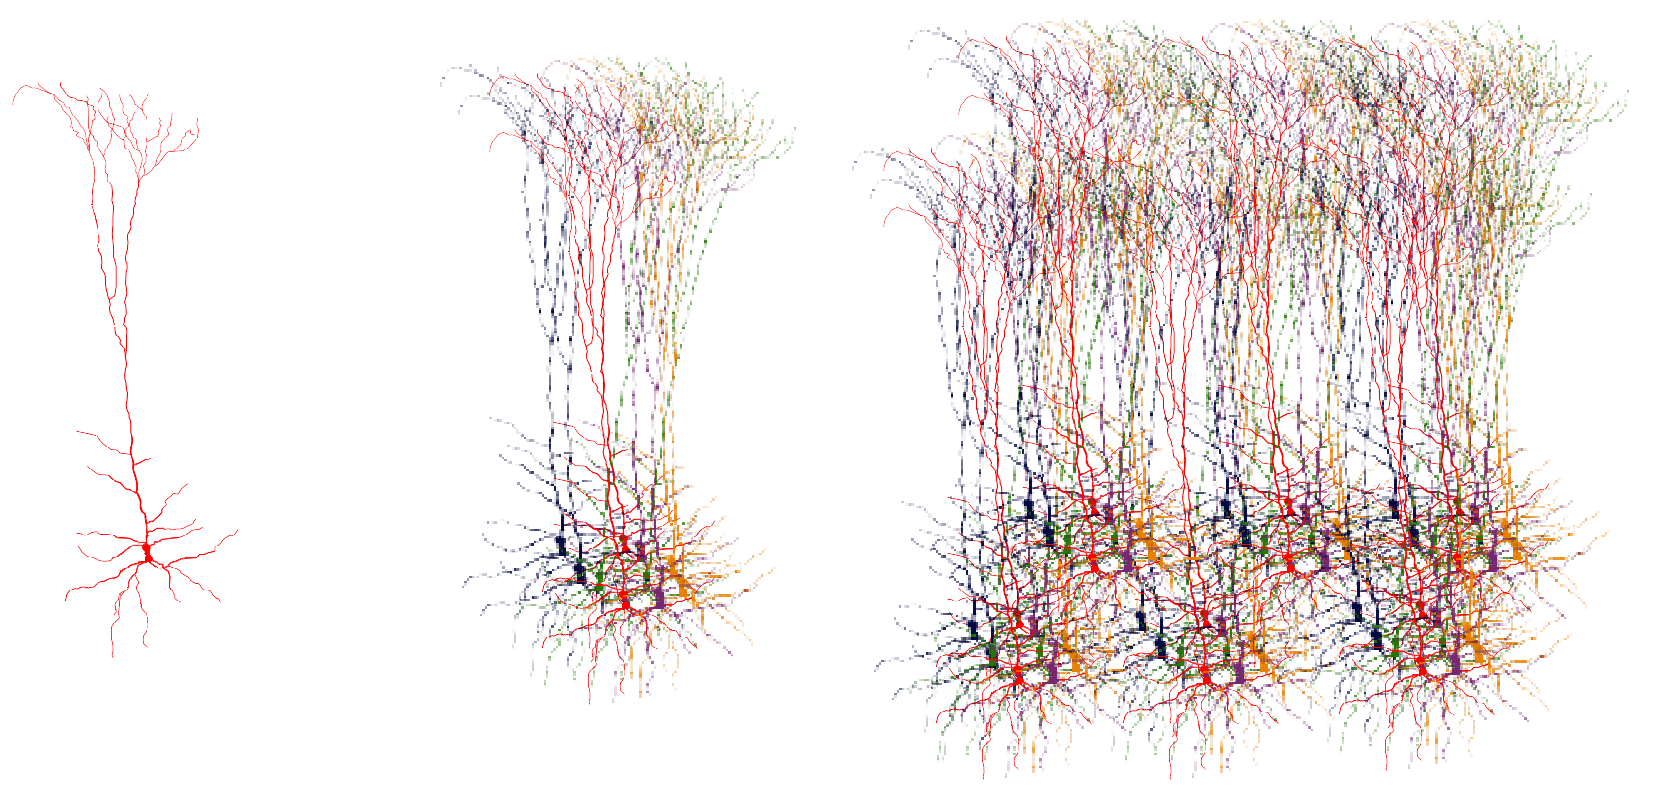
\includegraphics[width=1.0\textwidth]{Biological.png}
    \caption{Cortical tissue organization. Left: Pyramidal cell. The most common excitatory neuron in cortical tissue.
    Center: Cortical mini-column. A cluster on neural cells which responds to stimuli of similar characteristics.
    Right: Cortical Column. A group of mini-columns with a common receptive field location.
    Adapted from (Fabuio, Own work, CC BY 4.0, \url{https://commons.wikimedia.org/w/index.php?curid=60707501)}}
    \label{fig:Biological}
\end{figure}

One of the functional properties found in many of these networks is adaptation to contextual stimuli \cite{KRAUSE201436,doi:10.1167/16.13.1}. This mechanism is thought to enhance efficiency in the codification of sensory information. For instance, a reduction in the responses to frequent sounds by means of inhibitory networks, may enhance cortical sensitivity to rare sounds that may represent unexpected events~\cite{Natan2015ComplementaryCO,nachum_2003,Javitt11962}.

Finally, recent findings in neuroscience show that mammalian cortex processes information by means of \glspl{sdr}~\cite{barth_2012}. This mechanism allows robust and low-error-rate discrimination of stimuli representations minimizing the neuronal activation during the task in relation to the neural resources available for the representation~\cite{ahmad_2016}. Hawkins et al. \cite{hawkins_2016} hypothetize that one of the mechanisms that might be involved in cortical networks in order to achieve \glspl{sdr} implies the extended depolarization of the soma as the result of independent dendritic \gls{nmda} branch activations produced by the excitation of certain number of distal synapses~\cite{antic_2010, major_2013}.

In the present work the above mentioned anatomical and neurophysiological features of the mammalian cortex are gathered as potentially relevant in order to attain phonetic invariance in the mammalian auditory cortex. Our pyramidal neuron model dissociates proximal from distal dendritic branches (Fig.~\ref{fig:PyramidalCell}). Proximal dendrites act as a homogeneous set receiving only afferent information. Information in proximal dendrites determines a bunch of neural units in a \gls{cc} which could be activated depending on the previous activations in the same as well as in neighboring \glspl{cc}.

\begin{figure}[h!]
    \centering
    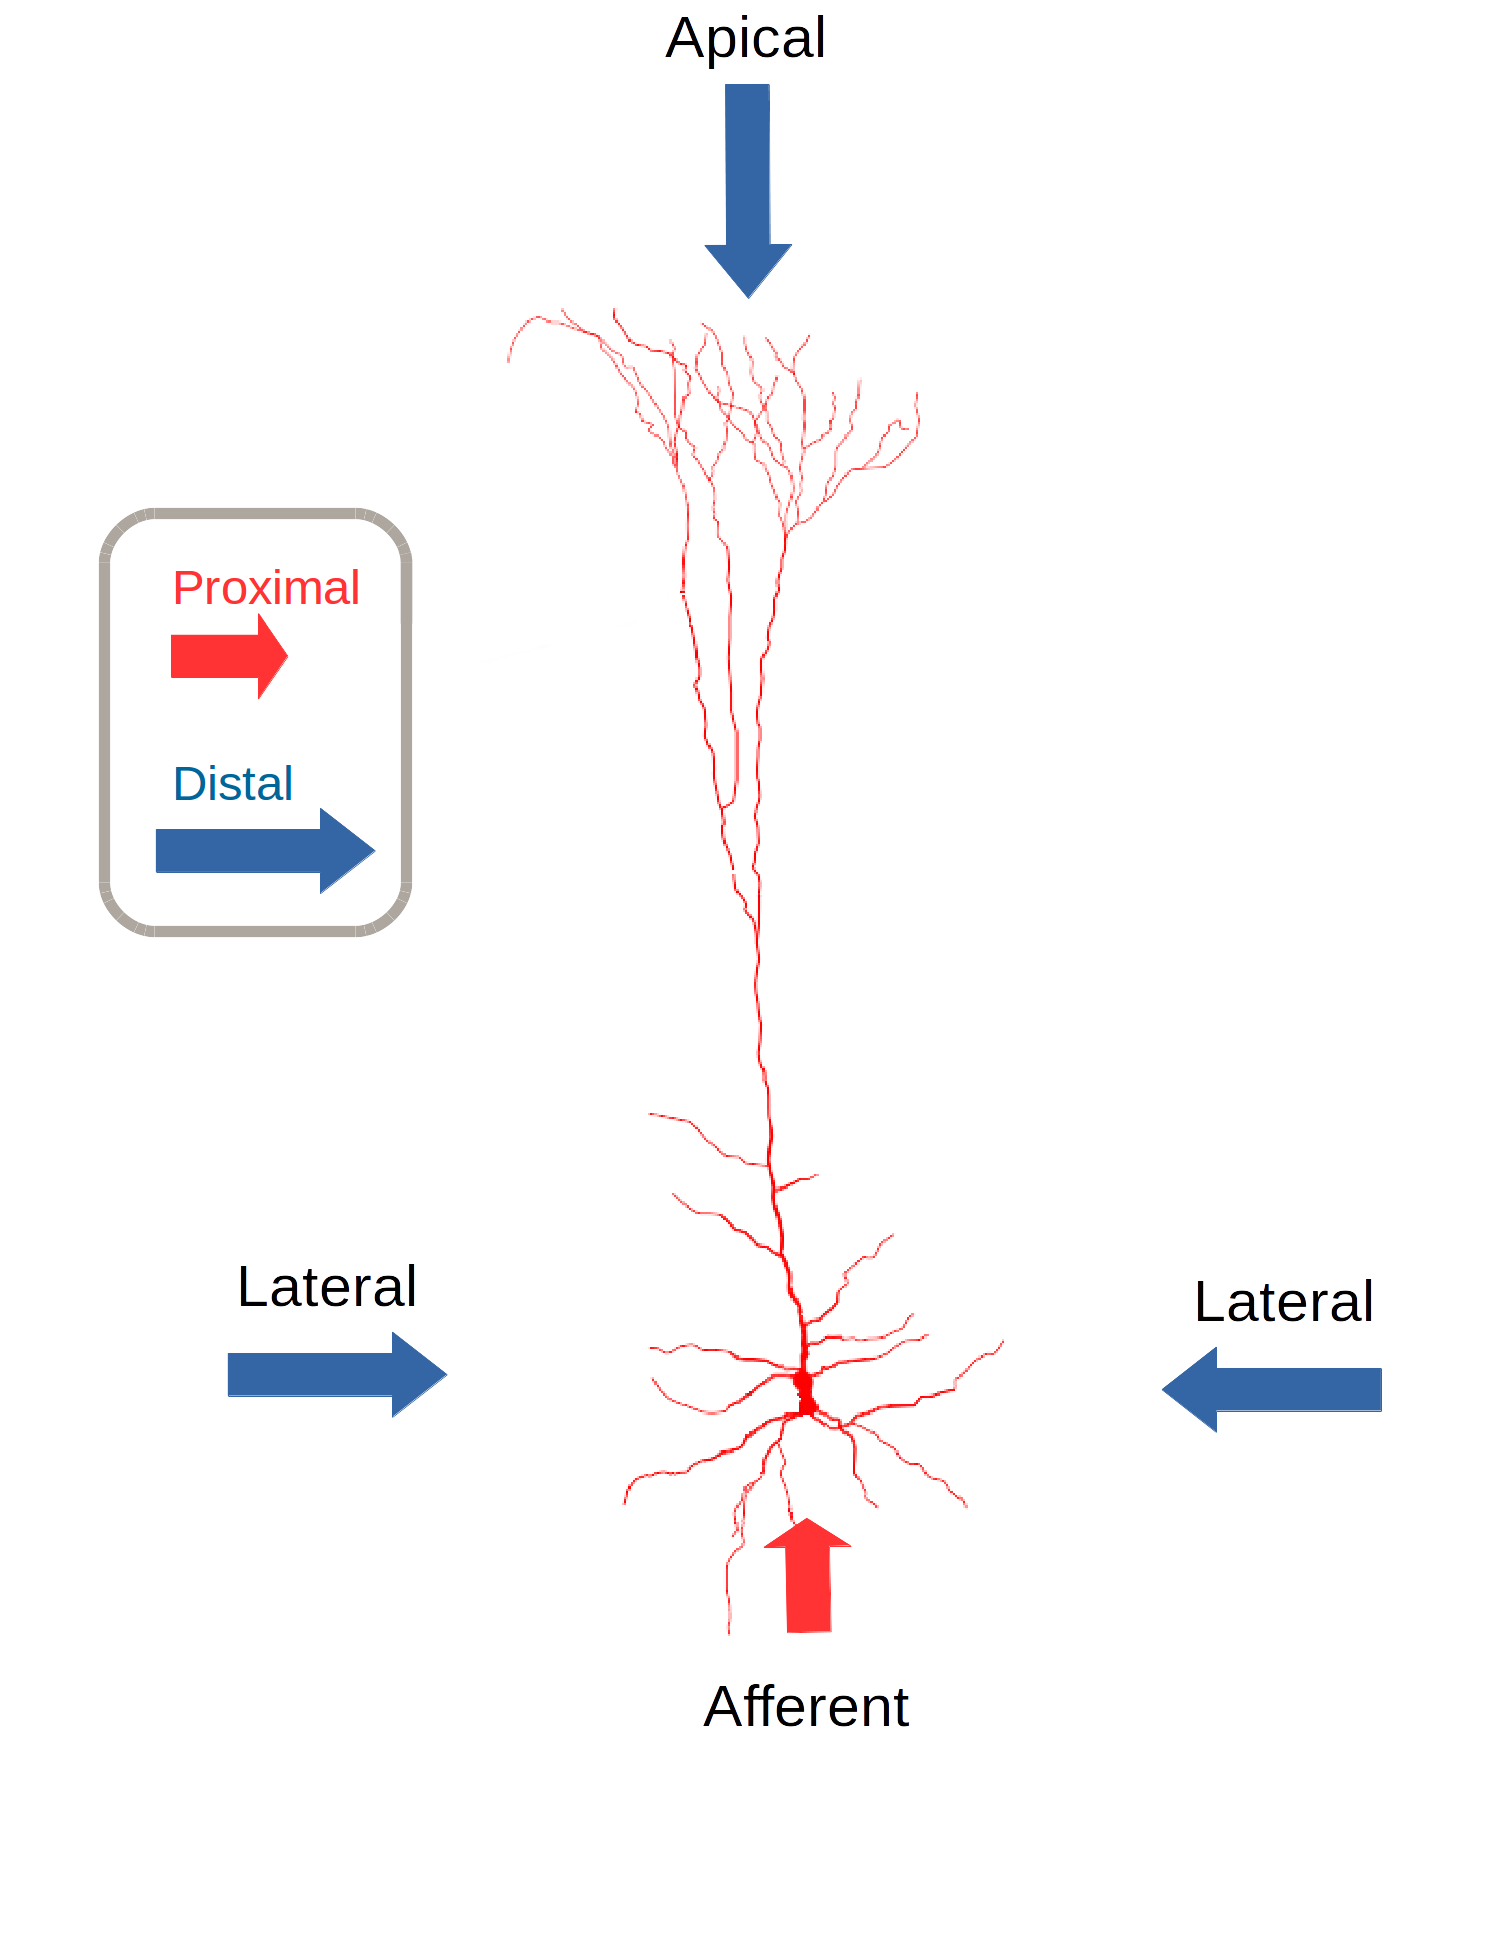
\includegraphics[width=0.5\textwidth]{PyramidalCell.png}
    \caption{Connectivity profile of a pyramidal neural unit in the \gls{el}.
    Proximal connections are formed only by afferent connections from the \gls{mrstsa}
    while distal connections are formed by lateral and apical connections from neighboring columns and
    from columns in another cortical layer above respectively.
    The \gls{el} is the most important stage in our computational approach while the \gls{mrstsa} pre-processes the audio corpora in order to feed the \gls{el}.
    Adapted from 
    (Fabuio - Own work, CC BY 4.0, \url{https://commons.wikimedia.org/w/index.php?curid=60707501)}}
    \label{fig:PyramidalCell}
\end{figure}

Distal dendrites receive only lateral and apical information acting as independent detectors. Distal dendritic information pre-activates neural units putting them in a predictive state in order to receive future afferent information.

We test those principles paying special attention to temporal dynamics of speech, which play the most important role in linguistic contrasts~\cite{doi:10.1098/rstb.1992.0070}. We use a completely unsupervised and biologically-inspired computational model, since we aim to mimic infant incidental phonetic acquisition in whose circumstances no supervision could be justified. Our model produces levels of phonetic classification accuracy similar to those of state-of-the-art deep pattern classification approaches. We therefore propose an alternative path towards addressing phonetic discrimination based on observing structural and functional properties present in the mammalian cortex.
}













\iftoggle{DEBUG}{
\section{Materiales y Métodos}
}{
\section{Materials and methods}
}







\iftoggle{DEBUG}{
\subsection{Generación de Corpus}
\label{CorpGen}

Generamos corpus de 500 palabras utilizando diez vocabularios diferentes con palabras monosilábicas, bisilábicas y tri-silábicas elegidas de manera aleatoria del idioma Inglés y utilizando el sintetizador \gls{festival} \cite{festival2014}.


Generamos archivos de marcado de lenguaje con SABLE \cite{sable}. Con tales archivos instruimos \gls{festival} para que genere corpus con 500  palabras de vocabularios de 5 palabras utilizando diez voces diferentes disponibles en el sintetizador.

La organización de los corpus presenta ciertas reglas y restricciones a los fines de evitar sesgos en los procesos de entrenamiento. Las voces se van eligiendo secuencialmente (seudo-aleatoriamente) con la restricción de que ninguna voz se puede utilizar por segunda vez hasta que la totalidad de las voces hayan tenido su turno. Cada voz se utiliza para producir dos palabras por turno--de manera pseudo-aleatoria--y ninguna palabra es repetida hasta que todas las palabras son producidas por tal voz.


Utilizamos dos conjuntos de voces, cada uno con 10 voces de origen Inglés provistos por Festival. El primer conjunto consistía de 8 voces masculinas y 2 femeninas: \texttt{cmu\_us\_fem\_cg, cmu\_us\_gka\_cg, cmu\_us\_ksp\_cg, cmu\_us\_rxr\_cg, cmu\_us\_jmk\_cg, cmu\_us\_rms\_cg, cmu\_us\_slt\_cg, cmu\_us\_jmk\_arctic\_clunits, cmu\_us\_rms\_arctic\_clunits, cmu\_us\_slt\_arctic\_clunits}. El segundo conjunto consistía de 5 voces masculinas y 5 femeninas: \texttt{cmu\_us\_ahw\_cg, cmu\_us\_aup\_cg, cmu\_us\_axb\_cg, cmu\_us\_eey\_cg, cmu\_us\_awb\_cg, cmu\_us\_bdl\_cg, cmu\_us\_clb\_cg, cmu\_us\_ljm\_cg, cmu\_us\_bdl\_arctic\_clunits, cmu\_us\_clb\_arctic\_clunits}.

Cada palabra en el archivo de audio es seguida por una brecha de silencio cuya duración equivale a la pronunciación de la palabra \texttt{cat} producida por la misma voz utilizada para producir la última palabra. Utilizamos el programa \texttt{text2wave} provisto por Festival para generar un archivo de extensión \texttt{wav} desde el archivo SABLE.

Generamos todos los conjuntos de datos (archivos de audio de los corpus) utilizados en el presente trabajo para entrenar la \gls{el} y las \glsfirst{svm} y para probar el \glsfirst{cstm} completo. Tal carpeta incluye un conjunto de 840 corpus distribuidos en dos corpus por cada configuración organizada por dos conjuntos de voces sintetizadas, tres condiciones silábicas y diez vocabularios distribuidos en 6 variantes acústicas aparte de los corpus en sus versiones originales. Las 6 variantes acústicas corresponden a: dos niveles de ruido blanco (19.8 dB y 13.8 dB \gls{snr} promedio \gls{rms} tasa de potensia), dos niveles de reverberación (\gls{rt} con valores de 0.61 segundos y 1.78 segundos) y variaciones de tono en ambas direcciones (de E a G y de E a C) \cite{dematties_dario_2019_2576130}.
}{
\subsection{Corpora generation}
\label{CorpGen}

We generate corpora of 500 words with mono, di and trisyllabic randomly chosen English words from 10 different vocabularies of five words
for each syllabic condition using \gls{festival} Synthesis \cite{festival2014}.

We generate cross synthesizer mark-up-language files with SABLE \cite{sable}.
In such files, we instruct \gls{festival} to generate corpora with 500 words from vocabularies of
5 words uttered by 10 different voices available from the synthesizer.

The organization of the corpora has certain rules and restrictions in order to avoid biases in the training processes.
The voices are sequentially chosen (pseudo-randomly) with the restriction that no voice could utter a second time until all the voices had uttered in their turns. Every voice utters two words per turn--in pseudo-random order--and no word is repeated until all the words are used by such voice. 

We use two sets of 10 different English speaking voices, each provided by Festival. Set one consisted of 8 male and 2 female voices: \texttt{cmu\_us\_fem\_cg, cmu\_us\_gka\_cg, cmu\_us\_ksp\_cg, cmu\_us\_rxr\_cg, cmu\_us\_jmk\_cg, cmu\_us\_rms\_cg, cmu\_us\_slt\_cg, cmu\_us\_jmk\_arctic\_clunits, cmu\_us\_rms\_arctic\_clunits, cmu\_us\_slt\_arctic\_clunits}. Set two had 5 male and 5 female voices: \texttt{cmu\_us\_ahw\_cg, cmu\_us\_aup\_cg, cmu\_us\_axb\_cg, cmu\_us\_eey\_cg, cmu\_us\_awb\_cg, cmu\_us\_bdl\_cg, cmu\_us\_clb\_cg, cmu\_us\_ljm\_cg, cmu\_us\_bdl\_arctic\_clunits, cmu\_us\_clb\_arctic\_clunits}.

Every word in the audio file is followed by a silence gap whose time is equivalent to the uttering time of the monosyllabic word \textit{cat}, uttered by the same voice used for the last word. We use the \texttt{text2wave} program provided by Festival in order to generate a \texttt{wav} file from the SABLE file.

We generated all the datasets (audio file corpora) employed in the present research to train the \gls{el} and the \glspl{svm} and to test the complete \gls{cstm}. This folder includes a set of 840 corpora which are distributed in 2 corpora for each configuration organized by 2 sets of synthesized voices, 3 syllabic conditions and 10 vocabularies all distributed in 6 acoustic variants, beyond the original version of the corpora. The 6 acoustic variants corresponds to: two levels of white noise (19.8 dB and 13.8 dB \gls{snr} average \gls{rms} power rate), two levels of reverberation (\gls{rt} value of 0.61 seconds and 1.78 seconds) and variations of pitch on both directions (from E to G and from E to C) \cite{dematties_dario_2019_2576130}.
}
























\iftoggle{DEBUG}{
\subsection{Modelo Computacional}
\label{model-implementation}

Proponemos un modelo computacional llamado \glsfirst{cstm}, que simula un parche de tejido cortical e incorpora organización columnar, formación micro-columnar espontánea, depolarización \gls{nmda} parcial y adaptación a activaciones contextuales. Simulamos células priramidales con conexiones próximas desde ramas dendríticas aferentes y conexiones distales desde ramas dendríticas laterales. Estímulos aferentes similares activan cúmulos de neuronas en localizaciones físicas próximas en una \gls{cc} de la misma manera en que la información aferente activa las minicolumnas que se encuentran en el tejido cortical.

La información aferente activa cúmulos diferentes de unidades en una \gls{cc} estableciendo una aproximación preliminar--y de alguna manera cruda--de las características fonéticas abstraídas desde el flujo de entrada auditivo. Nuestro modelo refina tales características crudas por medio de activaciones contextuales previas producidas en la misma y/o en \glspl{cc} vecinas. Tal información contextual se envía a cada \gls{cc} por medio de ramas dendríticas distales laterales que trabajan como elementos de procesamiento independientes en una célula. Las activaciones actuales en tales elementos dendríticos afectarán la manera en la cual las células reciben información aferente futura.

Teorías computacionales novedosas han aportado explicaciones posibles acerca del rol de las sinapsis distales relacionadas al
fenómeno \gls{nmda} \cite{hawkins_2016} combinándolo con con \gls{sdr_pl} \cite{ahmad_2016}. En nuestro modelo adoptamos un enfoque similar al adoptado en  \cite{hawkins_2016} en el que los patrones de activación actuales producen depolarización parcial de ciertas células por medio de conexiones con ramas dendríticas distales. Dicho estado de depolarización parcial se sostiene en el tiempo en algunas células dentro de
cúmulos de neuronas aferentemente excitados en el futuro. Las células parcialmente depolarizadas disparan primero que otras células en los cúmulos excitados, de esta forma evitan que tales otras células disparen utilizando inhibición GABAérgica lateral próxima, obteniendo así, \gls{sdr_pl}.

Adicionalmente, simulamos el crecimiento de sinapsis en ramas dendríticas distales por medio de mecanismos de \glsfirst{stdp} junto con
regulaciones homeostáticas. De esta forma, las sinapsis distales se establecerán solo entre células piramidales con patrones de activación secuenciales.
Los cúmulos aferentemente excitados que no tengan células parcialmente depolarizadas dispararán en conjunto produciendo un \glsfirst{mfe}
(ausencia de inhibición) como respuesta a una falla de predicción (estímulo secuencial inesperado en el flujo de datos); de lo contrario tales cúmulos responderán con eventos de disparo normales (inhibición y por lo tanto \glspl{sdr}) cuando el estímulo secuencial sea correctamente predicho.

Las \glspl{sdr} exhiben propiedades matemáticas interesantes las cuales les dan alto rechazo al ruido y gran tolerancia a fallas \cite{ahmad_2015}.
Estas son características típicas en el tejido cortical donde las células individuales están lejos de ser 100\% confiables y mueren y se regeneran constantemente. Para simular tal fenómeno, incorporamos características estocásticas por medio de las cuales las células neuronales dentro de los cúmulos activados aferentemente se escogen para ser activadas por medio de una distribución discreta cuyas probabilidades están determinadas por la excitabilidad aferente de las células individuales durante el entrenamiento.

De esta forma, la evolución de nuestra red no determina una neurona a disparar pero afecta sus probabilidades de hacerlo durante el entrenamiento. Adicionalmente y bajo condiciones específicas, las arborizaciones dendríticas aferentes se activan a sí mismas aleatoriamente con niveles cuyos valores limites son establecidos durante el entrenamiento.

Se ha demostrado que el overfitting--un fenómeno en el cual un modelo estadístico describe los ruidos o errores aleatorios en vez de su relación subyacente--se puede reducir considerablemente por medio de propiedades estocásticas en los procedimientos de entrenamiento aplicados a las redes neuronales (dropout)~\cite{JMLR:v15:srivastava14a}.

Para producir las entradas desde los flujos auditivos, nos basamos en el algoritmo \glsfirst{mrstsa}~\cite{chi_2005}. En nuestra implementación de software, seguimos principalmente su sección cortical en vez de su contraparte sub-cortical, incorporando diferentes fenómenos neurofisiológicos hallados en \gls{a1}~\cite{wang_1995} tales como modulación selectiva en simetría \cite{shamma_1993}, ancho de banda \cite{schreiner_1990}, y frecuencia \cite{shamma_1993,heil_1992,mendelson_1985}.



El \gls{cstm} consiste de dos partes: La capa \gls{mrstsa} y la \glsfirst{el}.

El algoritmo \gls{mrstsa}, que procesa las ondas de sonido para alimentar la entrada a la \gls{el}, es una técnica inspirada en Chi T. et al. \cite{chi_2005}. En su trabajo, hallazgos experimentales descubiertos en el sistema auditivo central se exploraron demostrando sus aplicaciones en la evaluación objetiva de la inteligibilidad del habla. Los autores indicaron que el modelo no fue biofísico en espíritu pero pudo proveer una interpretación desde datos fisiológicos posiblemente relevantes en el diseño de sistemas de ingeniería de sonido. En nuestra implementación del \gls{mrstsa}, seguimos los lineamientos principales de las representaciones corticales más altas desarrolladas en \cite{chi_2005}.

La \gls{el} convierte un arreglo multidimensional de números reales en una \gls{sdr} multidimensional. Esta etapa está compuesta por un conjunto de \glsfirst{som_pl} \cite{kohonen_2082, Kohonen:1989:SAM:69371} e incorpora fenómenos neurofisiológicos como organización columnar, formación micro-columnar espontánea aferente, arborizaciones dendríticas próximas y distales, interacción intercolumnar lateral por medio de activaciones \gls{nmda} de ramas dendríticas independientes, \gls{mfe_pl} con adaptación a estímulos contextuales, inhibición intracolumnar lateral próxima, \glsfirst{ltp}, \glsfirst{ltd}, \gls{stdp} y regulaciones homeostáticas en sinapsis distales.
}{
\subsection{Computational model}
\label{model-implementation}

We propose a computational approach called \gls{cstm}, which simulates a patch of cortical tissue and incorporates columnar organization, spontaneous micro-columnar formation, partial \gls{nmda} depolarization and adaptation to contextual activations. We simulate pyramidal cells with proximal connections from afferent dendritic branches and distal connections from lateral dendritic branches. Similar afferent stimuli activate clusters of neurons with proximal physical locations in a \gls{cc} in the same way that afferent information activates the mini columns found in cortical tissue.

Afferent information activates different clusters of units in a \gls{cc} establishing a first and raw approximation of the phonetic features abstracted from the input auditory stream. Our model fine-tunes such raw features by means of previous contextual activations produced in the same and/or in neighboring \glspl{cc}. Such contextual information is sent to each \gls{cc} by means of lateral distal dendritic branches which work as independent processing elements in a cell. Current activation in such dendritic elements will affect the way in which cells receives future afferent information.

Novel computational theories have posited a feasible explanation about the role of distal synapses related to \gls{nmda}
phenomenon \cite{hawkins_2016} by combining it with \glspl{sdr} \cite{ahmad_2016}. In our model, we adopt a similar approach to the one in \cite{hawkins_2016} in which current activation patterns produce partial depolarization of certain cells by means of distal dendritic branch connections. A state of partial depolarization is sustained in time in some cells within
future afferently excited clusters of neurons. Partially depolarized cells fire in advance with respect to other cells in the excited clusters, thereby preventing other cells from firing by means of proximal lateral GABAergic inhibition, obtaining in this way, \glspl{sdr}.

In addition, we simulate the growth of distal dendritic branch synapses by means of \gls{stdp} mechanisms together with
homeostatic regulations. In this way, distal synapses will be established only among pyramidal cells with sequential patterns
of activation. Afferently excited clusters which do not have partially depolarized cells,
will fire together producing a \gls{mfe}
(lack of inhibition) as a response to a prediction fault (unexpected sequential stimuli in the stream of data); otherwise they will respond with normal firing events (inhibition and therefore \glspl{sdr}) when the sequential stimulus is
correctly predicted.

\glspl{sdr} exhibit interesting mathematical properties which give them high noise rejection and fault tolerance \cite{ahmad_2015}.
These are typical characteristics in cortical tissue where individual cells are far from 100\% reliable and the cells die and regenerate continuously. To simulate this phenomenon, we incorporate stochastic characteristics by which neural cells inside afferently activated clusters are chosen to be active by a discrete distribution whose probabilities are determined by the afferent excitability of individual cells during training.

Hence, the evolution of our network does not predetermine a neuron to fire but biases its probability of doing so during training. Additionally and under specific conditions, afferent dendritic arborizations activate themselves at random with levels whose boundary values are established by learning. 

It has been shown that overfitting--a phenomenon in which a statistical model describes random error or noise instead of the underlying relationship--is greatly reduced by stochastic properties in training procedures applied to neural networks (dropout)~\cite{JMLR:v15:srivastava14a}.

In order to produce the inputs from auditory streams we base on \gls{mrstsa}~\cite{chi_2005}. In our software implementation, we primarily follow its cortical section rather than its sub-cortical counterpart, incorporating different neurophysiological phenomena found in \gls{a1}~\cite{wang_1995} such as symmetry \cite{shamma_1993}, bandwidth \cite{schreiner_1990}, and frequency modulation selectivity \cite{shamma_1993,heil_1992,mendelson_1985}.


The \gls{cstm} consists of two parts: The \glsfirst{mrstsa} layer and the \glsfirst{el}.

The algorithm \gls{mrstsa}, which processes the sound waves to feed inputs to the \gls{el}, is a technique inspired by Chi T. et al. \cite{chi_2005}. In their work, accumulating experimental findings from the central auditory system were exploited demonstrating its applications in the objective evaluation of speech intelligibility. As the authors pointed out, the model was not biophysical in spirit, but rather it abstracted from the physiological data an interpretation which was likely to be relevant in the design of sound engineering systems. In our \gls{mrstsa} implementation, we follow main guidelines from the higher cortical representations developed in \cite{chi_2005}.

The \gls{el} converts a multidimensional array of real numbers into a multidimensional \gls{sdr}. This stage is composed by a set of \glspl{som} \cite{kohonen_2082, Kohonen:1989:SAM:69371} and incorporates neurophysiological phenomena such as columnar organization, afferent spontaneous micro-columnar formation, proximal and distal dendritic arborization, lateral intercolumn interaction by means of independent dendritic \gls{nmda} branch activations, \glspl{mfe} with contextual stimulus adaptation, proximal lateral intracolumn inhibition, \gls{ltp}, \gls{ltd}, \gls{stdp} and distal synaptic homeostatic regulations.
}




























































\iftoggle{DEBUG}{
\subsubsection{Análisis Multiresolución Espectro-Temporal de Sonidos (AMRETS)}

Como se mensiona arriba, Chi T. et al. \cite{chi_2005} desarrollaron un modelo computacional de análisis auditivo inspirado en hallazgos psicoacústicos y
neurofisiológicos en etapas tempranas y centrales del sistema auditivo.

El algoritmo original tiene una etapa subcortical y una cortical.
Para la etapa subcortical, primero una transformada affine wavelet de la señal acústica
representa el análisis espectral realizado por el banco de filtros cocleares.
Segundo, las salidas del filtro coclear son transducidas en patrones del nervio auditivo
por medio de una etapa de células pilosas que consiste en un filtro pasa-alto,
una compresión no linear y un filtro pasa-bajo de fuga de membrana.
Tercero, una derivada de primer orden con respecto al eje tonotópico
seguida por un rectificador de media onda
simula la acción de una red inhibitoria lateral que se postula existe en el núcleo coclear,
el cual efectivamente realza la selectividad de frecuencia
del banco de filtros cocleares.
La salida final de la etapa se obtiene integrando
sobre una ventana angosta, con una constante de tiempo de 8 milisegundos, imitando
la subsecuente pérdida del bloqueo de fase observada en el mesencéfalo. 

La etapa cortical imita aspectos de las respuestas de etapas auditivas centrales más altas, especialmente \gls{a1}.
Funcionalmente, esta etapa estima el contenido de modulación espectral y temporal del espectrograma auditivo.
Lo hace computacionalmente por medio de un banco de filtros
que son selectivos a diferentes parámetros de modulación espectrotemporal
cuyo rango va de tasas lentas a rápidas temporalmente, y
de escalas finas a amplias espectralmente. Los \glsfirst{strf_pl}
de estos filtros también se centran en diferentes frecuencias a lo largo del eje tonotópico. 

En el presente trabajo, debido a que nuestro objetivo es integrar propiedades neurofisiológicas--principalmente centradas en las características corticales--seguimos
los lineamientos principales en la implementación de la sección cortical de tal modelo.
Como se muestra en la Fig.~\ref{fig:MRSTSA}, implementamos la etapa inicial en nuestro modelo con la aplicación de una \glsfirst{fft} al vector de audio
con una ventana de muestreo distinta para cada resolución.
Luego extraemos la densidad espectral de potencia de cada resolución.
De esta manera obtenemos un análisis espectral multiresolución de la señal de audio,
con una resolución espectral alta y temporal baja para ventanas de muestreo grandes y
viceversa.
Tales ventanas de tiempo diferentes en la \gls{fft},
incorporaron--al mismo tiempo--filtros pasa-bajo de fuga con una constante de tiempo para cada
resolución tomando en cuenta así la disminución del bloqueo de fase en el nervio auditivo. 
Luego aplicamos un \glsfirst{mfb} con 128 elementos para cada espectro
a los fines de representar el análisis espectral realizado por el banco de filtros de la cóclea.
Luego convolucionamos cada resolución obtenida en el último paso a lo largo de su eje tonotópico
con una función compleja de múltiple resolución cuya parte real
fue la función simétrica del Sombrero Mexicano y su parte imaginaria fue su transformada de Hilbert, la cual es antisimétrica.
Con esta estrategia simulamos los fenómenos de modulación selectiva a la simetría \cite{shamma_1993}, el ancho de banda \cite{schreiner_1990}
y la frecuencia \cite{shamma_1993,heil_1992,mendelson_1985}
hallados en \gls{a1} e incorporados en los algoritmos originales \cite{wang_1995}.

\begin{figure}[h!]
    \centering
    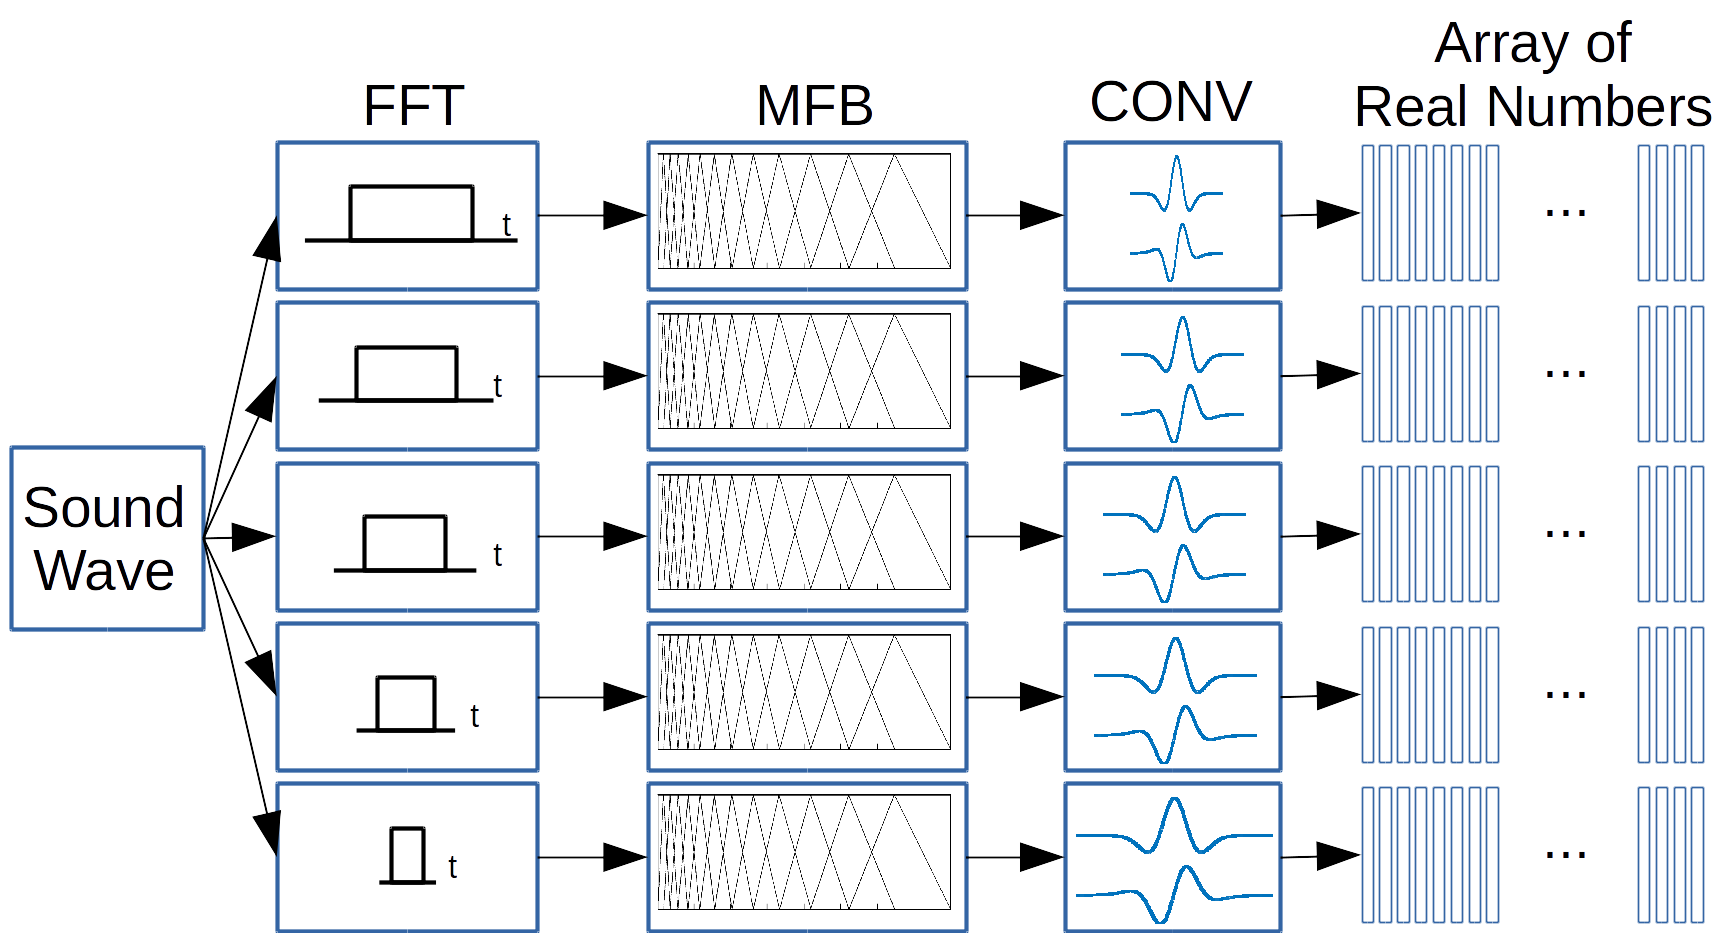
\includegraphics[width=0.8\textwidth]{MRSTSA.png}
    \caption{Algoritmo de \glsfirst{mrstsa}. Las ondas de sonido son procesadas por \glspl{fft} con ventanas de tiempo diferentes, luego, cada espectro es procesado por
	    un \glsfirst{mfb} y cada resolución es convolucionada con una señal compleja con un coeficiente diferente. Finalmente, cada coeficiente de filtro
	    se obtiene computando el módulo de la convolución y luego aplicando un control automático de ganancia.}
    \label{fig:MRSTSA}
\end{figure}

Finalmente, obtuvimos la amplitud de cada convolución y aplicamos normalización a cada ventana temporal
como un control automático de ganancia a los fines de priorizar la información entregada por la
configuración espectral y no los valores absolutos entregados por los filtros.

Por medio de estas restricciones tomamos en cuenta propiedades mecánicas y químicas de las células pilosas en el oido interno de los mamíferos
las cuales constituyen un mecanismo de transducción que parece adaptarse a la historia de estímulos recientes afectando su ganancia
\cite{eatock_2000,holt_2000,le_goff_2005}. 
Decidimos ser conservativos no incluyendo la dimensión de la intensidad de sonido solo incorporando la silueta de las respuestas de los filtros.
}{
\subsubsection{Multiresolution Spectro-Temporal Sound Analysis (MRSTSA)}

As mentioned above, Chi T. et al. \cite{chi_2005} developed a computational model of auditory analysis inspired by psychoacoustical and
neurophysiological findings in early and central stages of the auditory system.

The original algorithm has a subcortical and a cortical stage.
For the subcortical stage, first an affine wavelet transform of the acoustic signal
represents the spectral analysis performed by the cochlear filter bank.
Second, the cochlear filter outputs are transduced into auditory-nerve
patterns by a hair cell stage consisting of a high-pass filter,
a nonlinear compression and a membrane leakage low-pass filter.
Third, a first-order derivative with respect to the tonotopic axis
followed by a half-wave rectifier
simulates the action of a lateral inhibitory
network postulated to exist in the cochlear nucleus,
which effectively enhances the frequency
selectivity of the cochlear filter bank.
The final output of this stage is obtained by integrating
over a short window, with time constant of 8 ms, mimicking
the further loss of phase locking observed
in the midbrain.

The cortical stage mimics aspects of the responses of higher
central auditory stages, especially \gls{a1}.
Functionally, this stage estimates the
spectral and temporal modulation content of the auditory
spectrogram. It does so computationally via a bank of filters
that are selective to different spectrotemporal modulation parameters
that range from slow to fast rates temporally, and
from narrow to broad scales spectrally. The \glspl{strf}
of these filters are also centered at
different frequencies along the tonotopic axis.

In the present work, since we aim to integrate neurophysiological
properties--mainly centered in cortical features--we followed the main guidelines in the implementation of the cortical section of such model. 
As shown in Fig.~\ref{fig:MRSTSA}, we implemented the initial stage in our model with the application of \gls{fft} to the audio vector
with a different sample window for each resolution.
We then extracted the power spectral density from each resolution.
In this way we obtained a multiresolution spectral analysis of the audio signal,
with high spectral and low temporal resolution for wider sample windows and
vice versa.
Such different time windows in the \gls{fft},
incorporated--at the same time--leakage low-pass filters with a time constant for each
resolution accounting for decrease of phase-locking in the auditory nerve.
We then applied a \gls{mfb} with 128 elements to each spectrum
in order to represent the spectral analysis performed by the cochlear filter bank.
Then, we convolved each resolution obtained in the last step along its tonotopic axis
with a complex multiresolution function whose real part
was a symmetric Mexican hat function and its imaginary part was its antisymmetric Hilbert transform.
With this strategy we simulate the phenomena of symmetry \cite{shamma_1993}, bandwidth \cite{schreiner_1990}
and frequency modulation selectivity \cite{shamma_1993,heil_1992,mendelson_1985}
found in \gls{a1} and incorporated in the original algorithms \cite{wang_1995}.

\begin{figure}[h!]
    \centering
    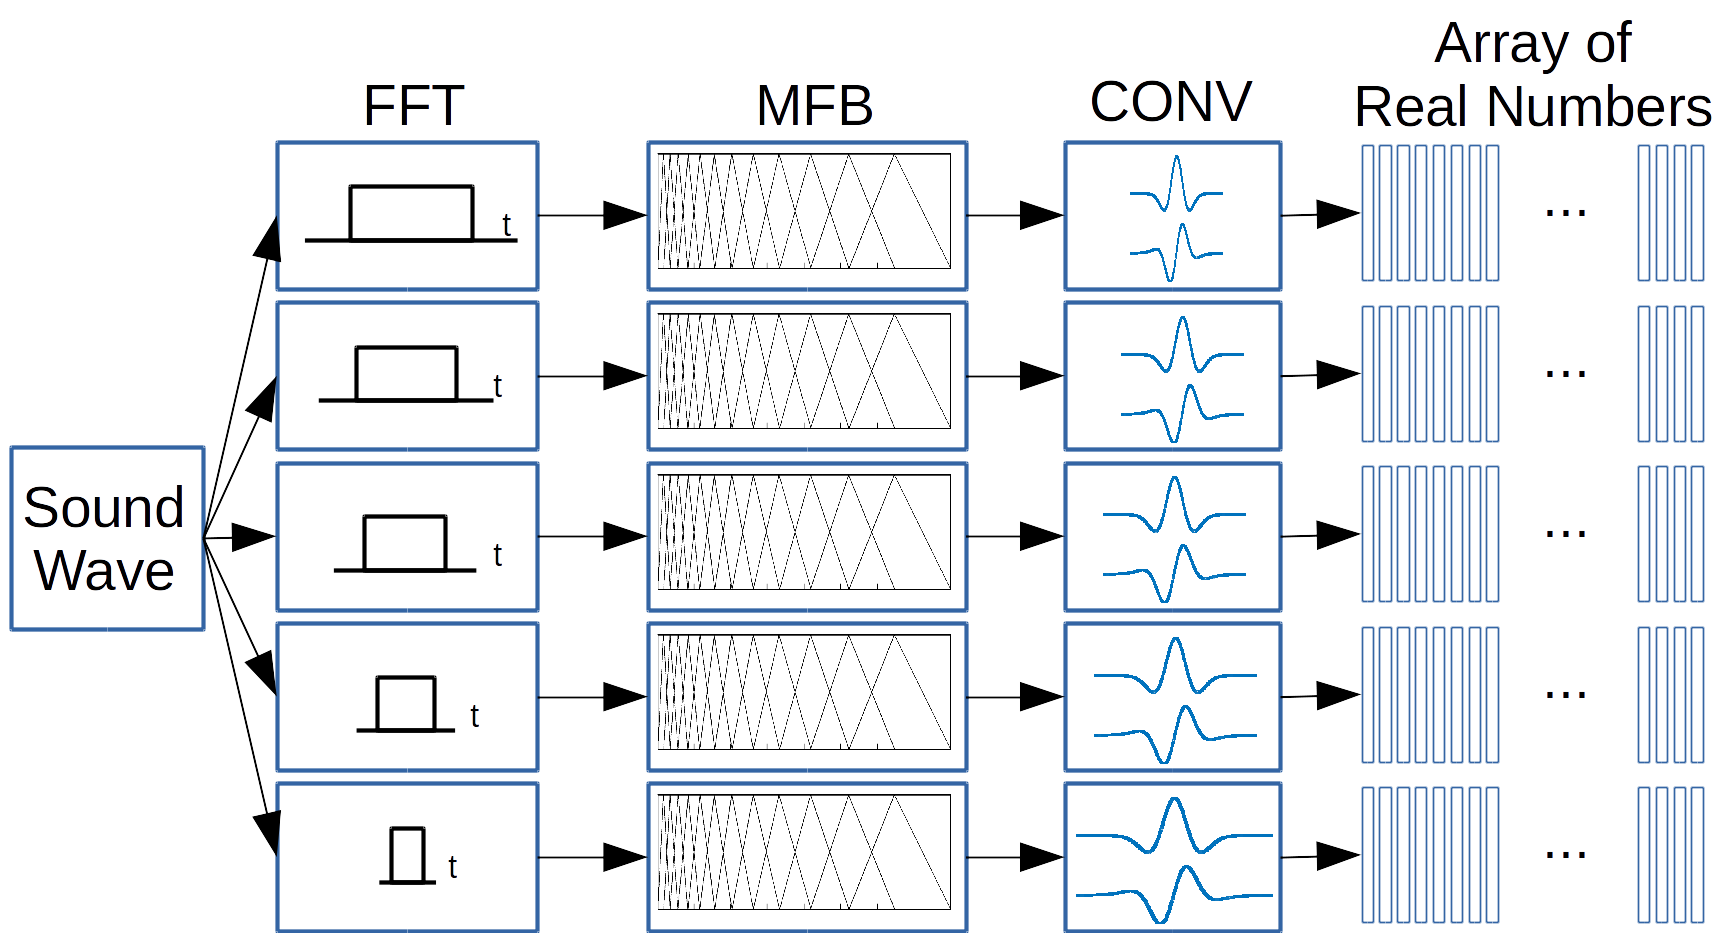
\includegraphics[width=0.8\textwidth]{MRSTSA.png}
    \caption{\glsfirst{mrstsa} algorithm. Sound waves are processed by \glspl{fft} with different time windows, then each spectrum is processed by
    a \glsfirst{mfb} and each resolution is convolved with a complex signal with a different coefficient. Finally, each filter coefficient
    is obtained computing the modulus from the convolution and then applying an automatic gain control.}
    \label{fig:MRSTSA}
\end{figure}

We obtained the magnitude of each convolution and applied normalization to each time window
as a mean of automatic gain control in order to prioritize the information delivered by the
spectral configuration and not the absolute values delivered by the filters. 

By means of this constraint we account for the mechanical and chemical properties of hair cells in the mammalian inner ear
which constitute a transduction mechanism that appears to adapt to recent stimulus history in a way that can affect its gain
\cite{eatock_2000,holt_2000,le_goff_2005}. 
We decided to be conservative, not including
sound intensity dimension but just the shape of the filter responses.
}















\iftoggle{DEBUG}{
\subsubsection{Capa Encoder (CE)}

La \gls{el} es la responsable de generar \glspl{sdr} desde las entradas entregadas por la etapa \gls{mrstsa}
descripta en la sección previa y desde la historia de activaciones en sus propias \glspl{cc}.

La \gls{el} simula un parche de tejido cortical llamado capa cortical utilizando un arreglo n-dimensional de estructuras complejas llamadas \glsfirst{csom_pl} que simulan \glspl{cc} en el cerebro.

Cada \gls{cc} en la \gls{el} se conecta al \gls{mrstsa} abajo por medio de conexiones aferentes. Cada \gls{cc} también se
conecta a \glspl{cc} vecinas--incluyendo posiblemente ella misma--en la \gls{el} por medio de conexiones laterales y
a \glspl{cc} desde otras capas corticales arriba por medio de conexiones apicales. Tal esquema de conexión se muestra en la Fig \ref{fig:EncoderColumnConnections}.

\begin{figure}[h!]
    \centering
    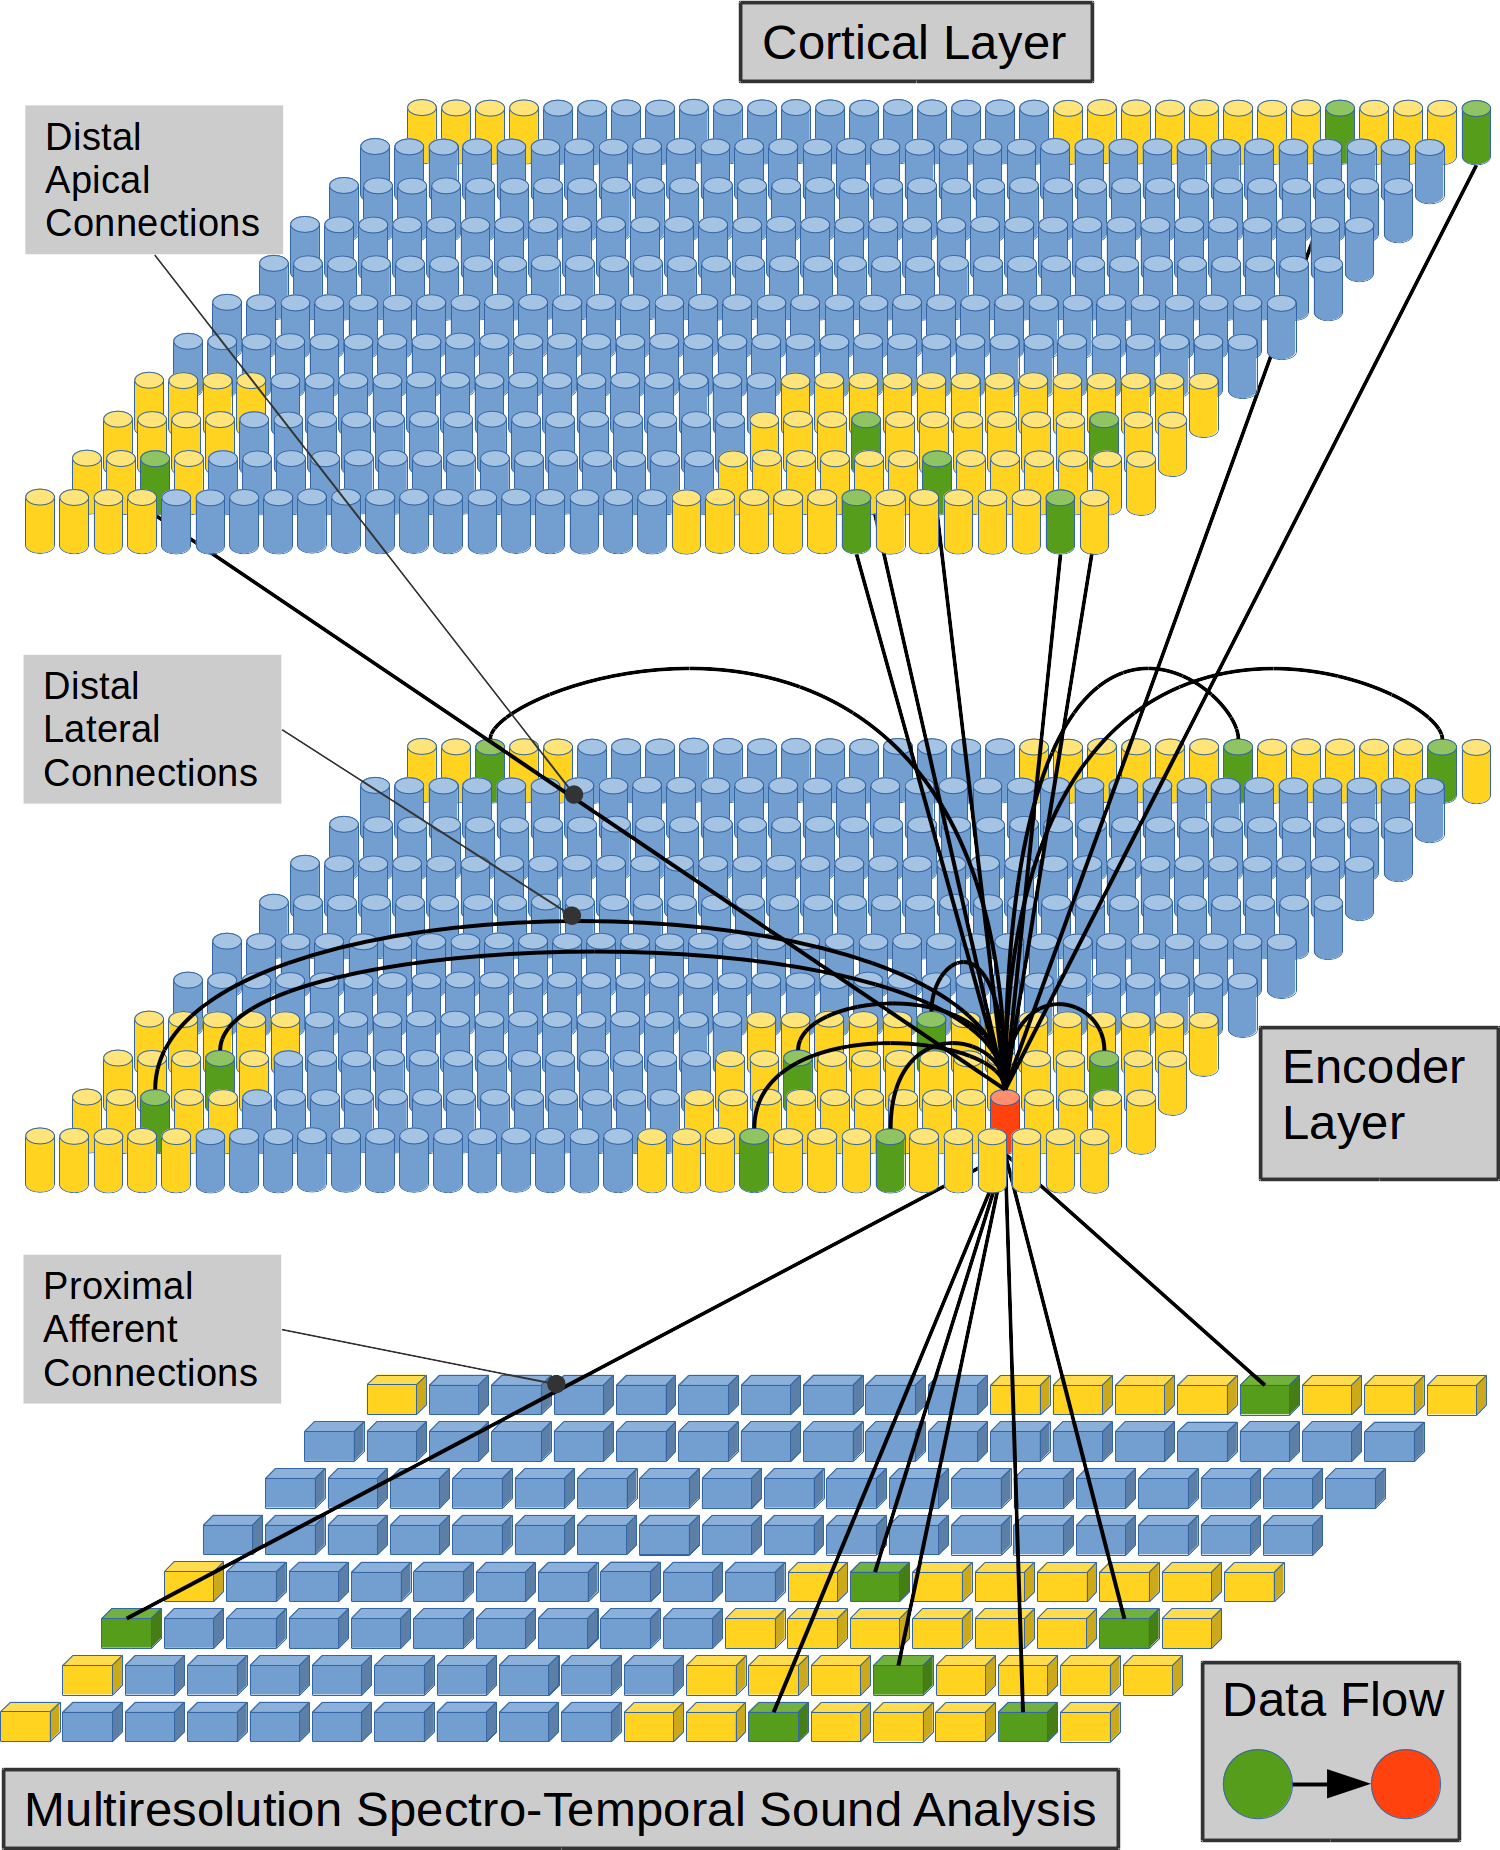
\includegraphics[width=0.6\textwidth]{EncoderColumnConnections.png}
    \caption{Esquema de conexión para una columna cortical en la Capa Encoder.
	    Cada cilindro en la \gls{el} y en el capa cortical superior representa una \gls{cc} en el tejido neuronal.
	    Cada prisma en el \gls{mrstsa} representa una variable de valor real.
	    Esta es la visualización de una \gls{cc} (en rojo) y sus de tres campos receptivos (en amarillo).
	    El campo receptivo de una \gls{cc} es un arreglo que define un conjunto de \glspl{cc}
	    con las cuales tal columna se podría conectar.
	    El campo receptivo de una \gls{cc} sobre el \gls{mrstsa} determina un arreglo de variables de valor real
	    con las cuales tal columna se podría conectar.
	    Un subconjunto de \glspl{cc} dentro de un campo receptivo (en verde) representa las \glspl{cc} que están realmente conectadas
	    con la \gls{cc} en rojo. Un escenario similar se podría describir para los prismas verdes sobre el \gls{mrstsa}.
	    El tamaño, propiedades de envoltura y el porcentaje de vínculos establecidos (en verde) dentro de un campo receptivo, son parámetros ajustables para el modelo.
	    En este trabajo, solo las conexiones laterales han sido implementadas ya que en la implementación actual no existen capas corticales superiores de las cuales traer conexiones apicales.}
    \label{fig:EncoderColumnConnections}
\end{figure}

Ambas conexiones laterales y apicales son conexiones de retroalimentación que constituyen canales de información contextual.
Estos canales ponen a la excitación aferente actual bajo el contexto de las activaciones previas.
Tales conexiones atenúan la actividad de algunas unidades permitiendo solo activaciones precisas
de unidades neuronales específicas en una \gls{cc} aferentemente excitada.
Tales activaciones precisas encuadran en los paradigmas secuenciales aprendidos por la red.

Hallazgos recientes en neurociencia \cite{Marques2018} sostienen la idea
de que la retroalimentación cerebral tiene la facultad potencial de acentuar representaciones visuales en tiempo y espacio
atenuando la actividad de ciertas células y permitiendo las activaciones de otras
que coinciden con sus representaciones.

En este trabajo solo implementamos conexiones laterales ya que
no hay capas superiores
de donde traer información apical en la presente implementación.

Cada unidad celular en una \gls{cc} tiene dos tipos de ramas dendríticas; próximas y distales.
Las ramas dendríticas próximas y distales conducen a conexiones próximas y distales en una célula respectivamente.
Las conexiones próximas y distales producen diferentes efectos en la plasticidad y activación de una unidad neuronal.
Las unidades neuronales en la \gls{el} simulan células piramidales en el tejido cortical en el cerebro.
La Fig \ref{fig:PyramidalCell} muestra el perfil de conectividad de tales unidades.
}{
\subsubsection{Encoder Layer (EL)}

The \gls{el} is responsible for generating \glspl{sdr} from the inputs delivered by the \gls{mrstsa} stage
described in the previous section and from the activation history in its own \glspl{cc}.

The \gls{el} simulates a patch of cortical tissue called \gls{cl}using an n-dimensional array of complex structures called \glspl{csom} that simulate \glspl{cc} in the brain.

Each \gls{cc} in the \gls{el} is connected to the \gls{mrstsa} below by means of afferent connections. It is also
connected to neighboring \glspl{cc}--including possibly itself--in the \gls{el} by means of lateral connections and
to \glspl{cc} from other \glspl{cl} above by means of apical connections. Such connection scheme is shown in Fig \ref{fig:EncoderColumnConnections}.

\begin{figure}[h!]
    \centering
    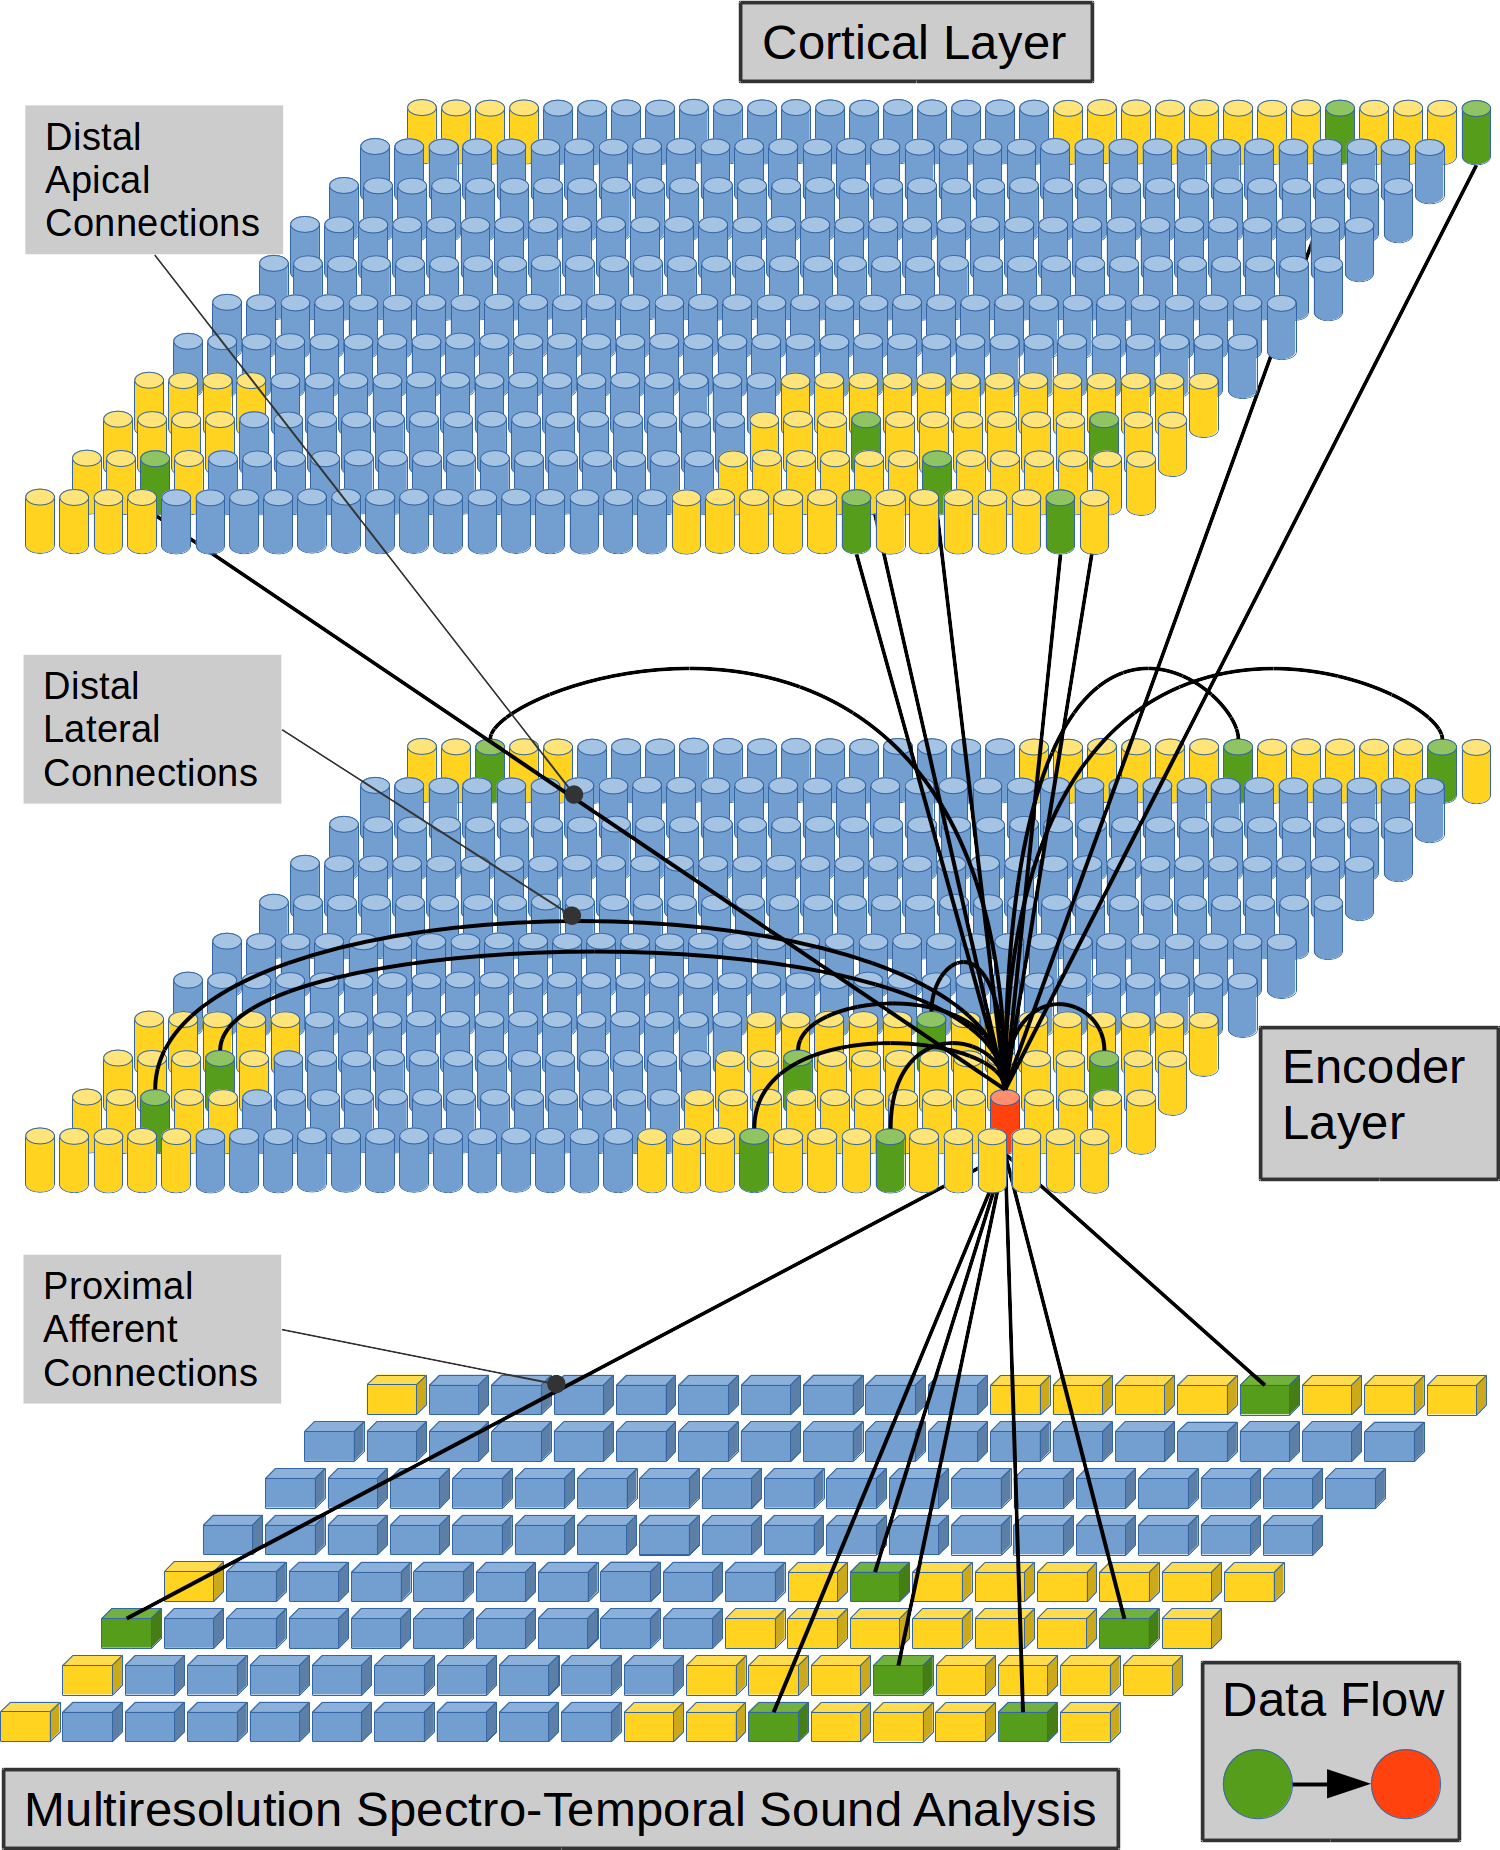
\includegraphics[width=0.6\textwidth]{EncoderColumnConnections.png}
    \caption{Connection scheme for a cortical column in the Encoder Layer.
	    Each cylinder in the \gls{el} and in the \gls{cl} represents a \gls{cc} in neural tissue.
	    Each prism in the \gls{mrstsa} represents a real valued variable.
	    This is a visualization of a \gls{cc} (in red) and its three receptive fields (in yellow).
	    The receptive field of a \gls{cc} is an array that defines a set of \glspl{cc}
	    with which such column could be connected.
	    The receptive field of a \gls{cc} on the \gls{mrstsa} determines an array of real valued variables
	    with which such column could be connected.
    A subset of \glspl{cc} in a receptive field (in green) represents the \glspl{cc} that are really
    connected with the \gls{cc} in red. A similar scenario could be described for the green prisms on
    the \gls{mrstsa}.
    The size, wrap-around property and percentage of established links (in green) inside a receptive field are tunable parameters for the model.
    In this work, only lateral connections have been implemented since in the current implementation there are no upper cortical layers from which
    to bring apical connections.}
    \label{fig:EncoderColumnConnections}
\end{figure}

Both lateral and apical are feedback connections that constitute contextual information channels. 
These channels put the current afferent excitation under the context of previous activations.
Such connections damp the activity of some units allowing only the precise activations
of specific neural units in an afferently excited \gls{cc}.
Such precise activations match the sequential paradigms learned by the network.

Recent findings in neuroscience \cite{Marques2018} support the idea 
that feedback could potentially enhance visual representations in time and space
damping the activity of certain cells while allowing the activations  of others
which agree with their predictions.

In the present work we only implement lateral connections since
there are no upper layers 
from which to bring apical information in the present implementation.

Each cell unit in a \gls{cc} has two types of dendritic branches; proximal and distal.
Proximal and distal dendritic branches lead to proximal and distal connections in a cell unit respectively.
Proximal and distal connections produce different effects on a neural unit's plasticity and activation.
Neural units in the \gls{el} simulates pyramidal cells in cortical tissue in the brain.
Fig \ref{fig:PyramidalCell} shows the connectivity profile in such units. 
}





























%\subsubsection{Conexiones Dendríticas Próximas}


\iftoggle{DEBUG}{
En referencia a las conexiones dendríticas próximas en la \gls{el}, cada unidad neuronal en una \gls{cc} tiene el mismo conjunto de
conexiones próximas al \gls{mrstsa} (Fig \ref{fig:EncoderProximalConnections}).
Tales conexiones constituyen un espacio multidimensional de números reales.
Para adquirir la distribución estadística de tal espacio real multidimensional utilizamos
un \gls{som} multidimensional en cada columna cortical (Alg.~\ref{csom_proximal_synapses}).

\begin{figure}[h!]
    \centering
    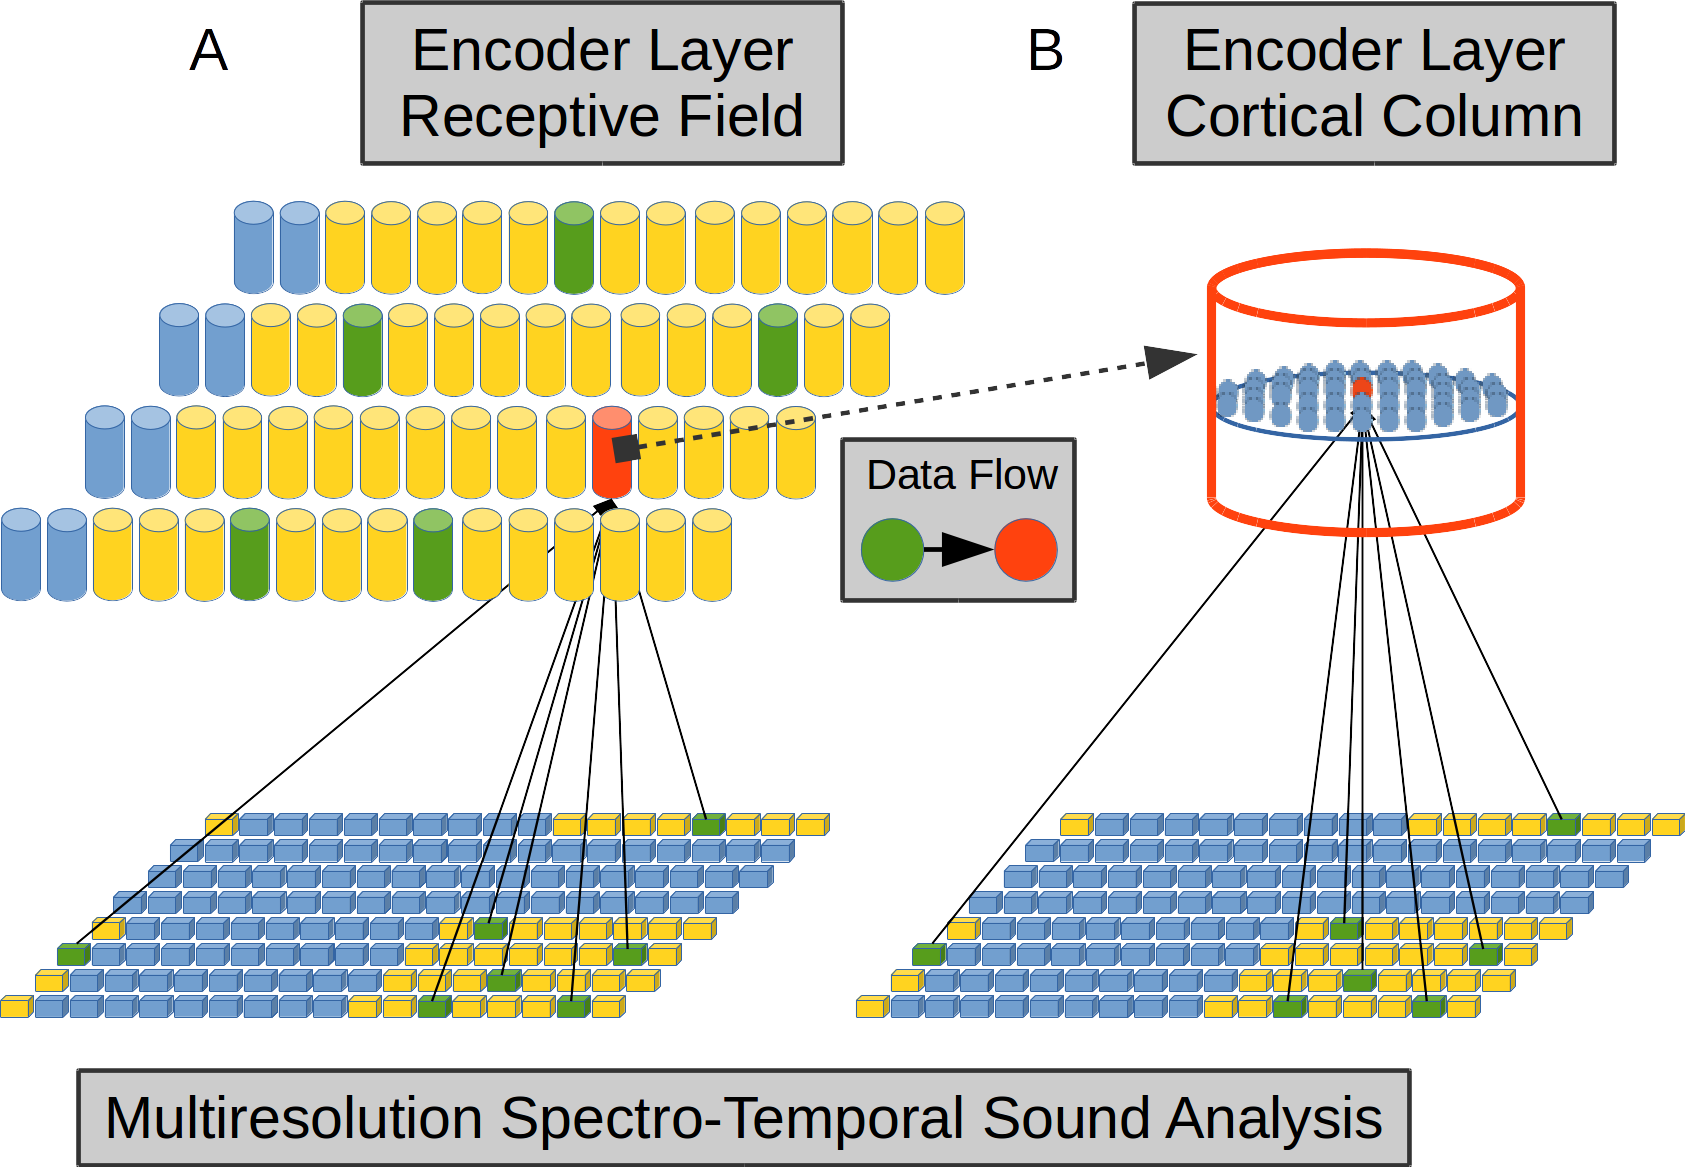
\includegraphics[width=0.8\textwidth]{EncoderProximalConnections.png}
    \caption{Conexiones próximas de la \glsfirst{el}. Cada \gls{cc} en la \gls{el}--ejemplificada aquí en color rojo--tiene su campo receptivo sobre el \gls{mrstsa}--en amarillo.
	    (A) Un conjunto de componentes del \gls{mrstsa}--en color verde dentro del campo receptivo--se ecoje aleatoriamente para ser conectado con tal \gls{cc}.
	    (B) Cada unidad neuronal en tal \gls{cc} se conecta con el mismo conjunto de componentes en el \gls{mrstsa}.}
    \label{fig:EncoderProximalConnections}
\end{figure}


\begin{algorithm}
	\caption{\texttt{Plasticity in Proximal Synapses}. \glsfirst{som} algorithm.}
\label{csom_proximal_synapses}
\begin{algorithmic}[1]
	\STATE{given an \texttt{input} vector, find the nearest \texttt{unit} to such \texttt{input} vector in the input space}
	\STATE{move such \texttt{unit} towards the \texttt{input} vector in the input space (the magnitude of such movement depends on the learning rate)}
	\STATE{also move neighbor \texttt{units} to the nearest one towards the \texttt{input} vector (the magnitude of such movement depends on the learning rate and on a neighborhood measure over the topology of the network of units)}
\end{algorithmic}
\end{algorithm}

Un \gls{som} es un algoritmo de clusterizado no supervisado que representa una distribución multidimensional continua
en una distribución multidimensional discreta de unidades neuronales \cite{Kohonen:1989:SAM:69371, kohonen_2082}.
De esta forma se termina con un arreglo de unidades de $m$ dimensiones en el cual cada unidad
representa un conjunto de vectores desde una distribución continua en un espacio de entrada de $n$ dimensiones.
Generalmente, $m < n$ para reducir la dimensionalidad en la representación discreta.
Agregamos tal restricción en nuestro algoritmo columnar.

En el algoritmo \gls{som}, cada vector de entrada debe estar completamente determinado.
En nuestro caso, varios elementos en las entradas desde el \gls{mrstsa} podrían ser nulos,
y considerar tales entradas nulas podría perjudicar el aprendizaje.
Por lo tando, cada vector de entrada podría no tener la información de cada componente disponible.
A tales efectos, incorporamos un mecanismo estocástico en la \gls{el} para lidiar con tal situación.
Hicimos que cada conexión aferente aprenda límites estadísticos desde sus entradas correspondientes.
Establecimos márgenes mínimos y máximos en cada conexión próxima en la \gls{el}.
Tal margen es consistente con la distribución estadística en la historia de su entrada correspondiente.
Cuando una entrada aferente está indeterminada, en un contexto en el que algunas entradas tienen información disponible,
la \gls{el} escoje el valor de la entrada indeterminada aleatoriamente
entre los límites aprendidos desde tal entrada.

Llamamos a nuestra implementación del algoritmo \gls{som}, \gls{ssom}.
El algoritmo \gls{ssom} simula interacción intra-columnar lateral, \gls{ltp} y \gls{ltd}.
También disocia las entradas dendríticas próximas de las dendritas distales, ya que
modifica  las conexiones próximas siguiendo la distribución estadística desde el \gls{mrstsa}
independientemente de las unidades que disparan en la \gls{cc}.
Esta independencia en la plasticidad de las entradas dendríticas próximas se apoya en la propiedad
hallada en el tejido cortical por medio de la cual existe plasticidad dendrítica
en el contexto de la depolarización parcial del soma \cite{reiter_1998}--es decir, sin un \glsfirst{ap}.

El termino \textit{Estático} viene del hecho de que los patrones aprendidos desde las dendritas aferentes próximas
no toman en cuenta la historia contextual en la evolución dinámica del algoritmo.
}{
In reference to proximal connections in the \gls{el}, each neural unit in a \gls{cc} has the same set of
proximal connections to the \gls{mrstsa} (Fig \ref{fig:EncoderProximalConnections}).
Such connections constitute a multidimensional space of real numbers.
In order to acquire the statistical distribution in such multidimensional real space we use
a multidimensional \gls{som} in each cortical column (Alg.~\ref{csom_proximal_synapses}).

\begin{figure}[h!]
    \centering
    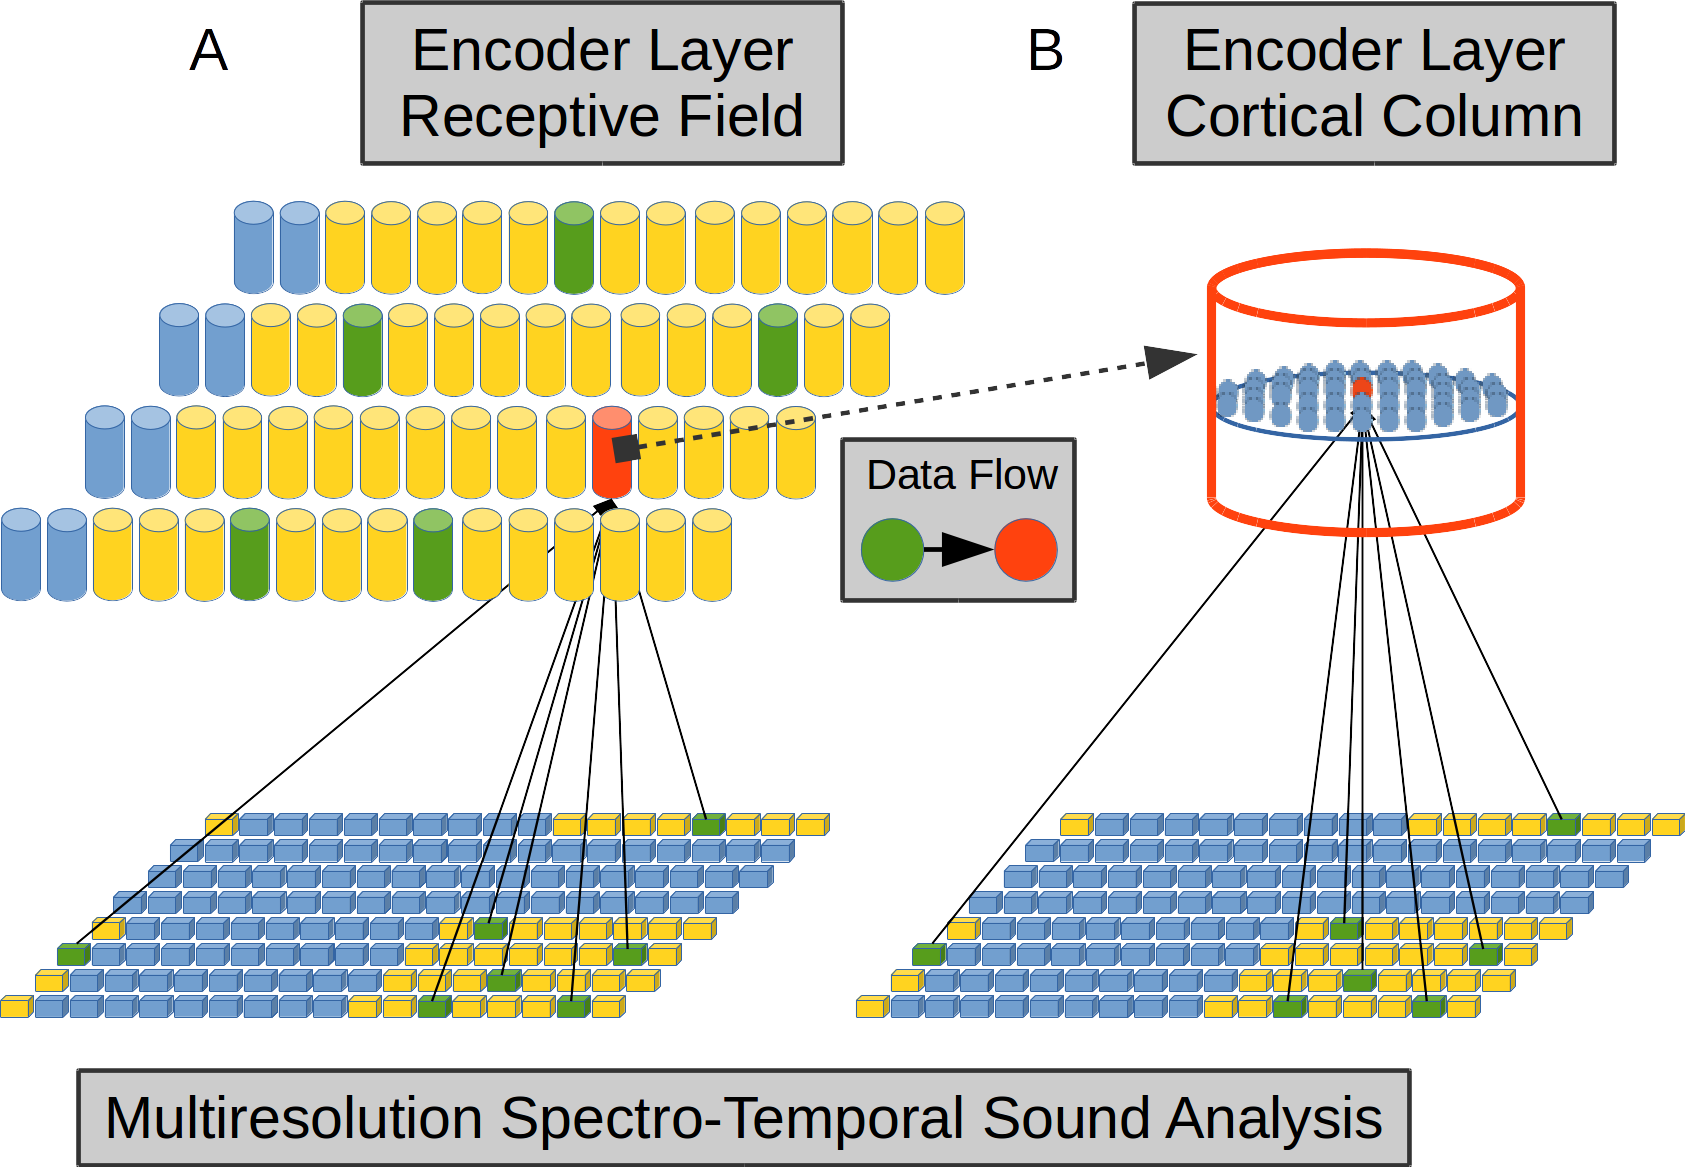
\includegraphics[width=0.8\textwidth]{EncoderProximalConnections.png}
    \caption{\glsfirst{el} proximal connections. Each \gls{cc} in the \gls{el}--exemplified here in red--has its receptive field over the \gls{mrstsa}--in yellow.
    (A) A set of \gls{mrstsa} components--in green inside the receptive field--is randomly chosen to be connected with such \gls{cc}.
    (B) Each neural unit in such \gls{cc} is connected with the same set of \gls{mrstsa} components.}
    \label{fig:EncoderProximalConnections}
\end{figure}


\begin{algorithm}
	\caption{\texttt{Plasticity in Proximal Synapses}. \glsfirst{som} algorithm.}
\label{csom_proximal_synapses}
\begin{algorithmic}[1]
	\STATE{given an \texttt{input} vector, find the nearest \texttt{unit} to such \texttt{input} vector in the input space}
	\STATE{move such \texttt{unit} towards the \texttt{input} vector in the input space (the magnitude of such movement depends on the learning rate)}
	\STATE{also move neighbor \texttt{units} to the nearest one towards the \texttt{input} vector (the magnitude of such movement depends on the learning rate and on a neighborhood measure over the topology of the network of units)}
\end{algorithmic}
\end{algorithm}

A \gls{som} is an unsupervised clustering algorithm which distributes a continuous multidimensional distribution
in a discrete multidimensional distribution of units \cite{Kohonen:1989:SAM:69371, kohonen_2082}.
In this way we ended up with an array of units of $m$ dimensions in which each unit
represents a set of vectors from the continuous distribution in an input space of $n$ dimensions.
Generally, $m < n$ in order to reduce the dimensionality in the discrete representation.
We added such restriction in our columnar algorithm.

In the \gls{som} algorithm, each input vector has to be completely determined.
In our case, several elements in the inputs from the \gls{mrstsa} could be null,
and considering such null inputs could inpair learning. 
Hence, each input vector could not have the information of each of its components available.
We incorporated a stochastic mechanism in the \gls{el} in order to deal with such situation.
We made each afferent connection to learn statistical boundaries from its corresponding input.
We establish a minimum-maximum margin in each proximal connection in the \gls{el}.
Such margin is consistent with the statistical distribution in the history of its corresponding input.
When an afferent input is undetermined, in a context in which some afferent inputs have
available information,
the \gls{el} chooses
the value in the undetermined input
randomly
between the boundaries learned for such input.

We call our implementation of the \gls{som} algorithm, \gls{ssom}.
The \gls{ssom} algorithm accounts for proximal lateral intra-column interaction, \gls{ltp} and
\gls{ltd}.
It also dissociates proximal dendritic inputs from distal dendrites, since
it modifies
proximal connections
following the statistical distribution from the
\gls{mrstsa} independently of the units that fire in such \gls{cc}.
This independence in the plasticity of the proximal dendritic inputs
is supported by
the
property
found in cortical tissue by means of which there is dendritic plasticity
in the context of partial depolarization of the soma \cite{reiter_1998}--that is, without an \gls{ap}. % Citation needed here

The term \textit{static} comes from the fact that the patterns learned from proximal afferent
dendrites do not account for the contextual history in the dynamic evolution
of the algorithm.
}




























%\subsubsection{Conexiones Dendríticas Distales}


\iftoggle{DEBUG}{
En términos de las ramas dendríticas distales, cada \gls{cc} en la \gls{el} se conecta con otras \glspl{cc}--en verde en la Fig \ref{fig:EncoderColumnConnections}--por medio de tales ramas dentro de los campos receptivos--en amarillo en la Fig. \ref{fig:EncoderColumnConnections}--desde la misma \gls{el} y desde otra capa cortical arriba.
Cada vínculo entre la \gls{cc} roja y la \gls{cc} verde--Fig. \ref{fig:DistalDendrites} A--
simboliza el hecho de que cada unidad celular en
la \gls{cc} roja está vinculada con un subconjunto diferente de unidades celulares en la \gls{cc} verde--Fig. \ref{fig:DistalDendrites} B.

\begin{figure}[h!]
    \centering
    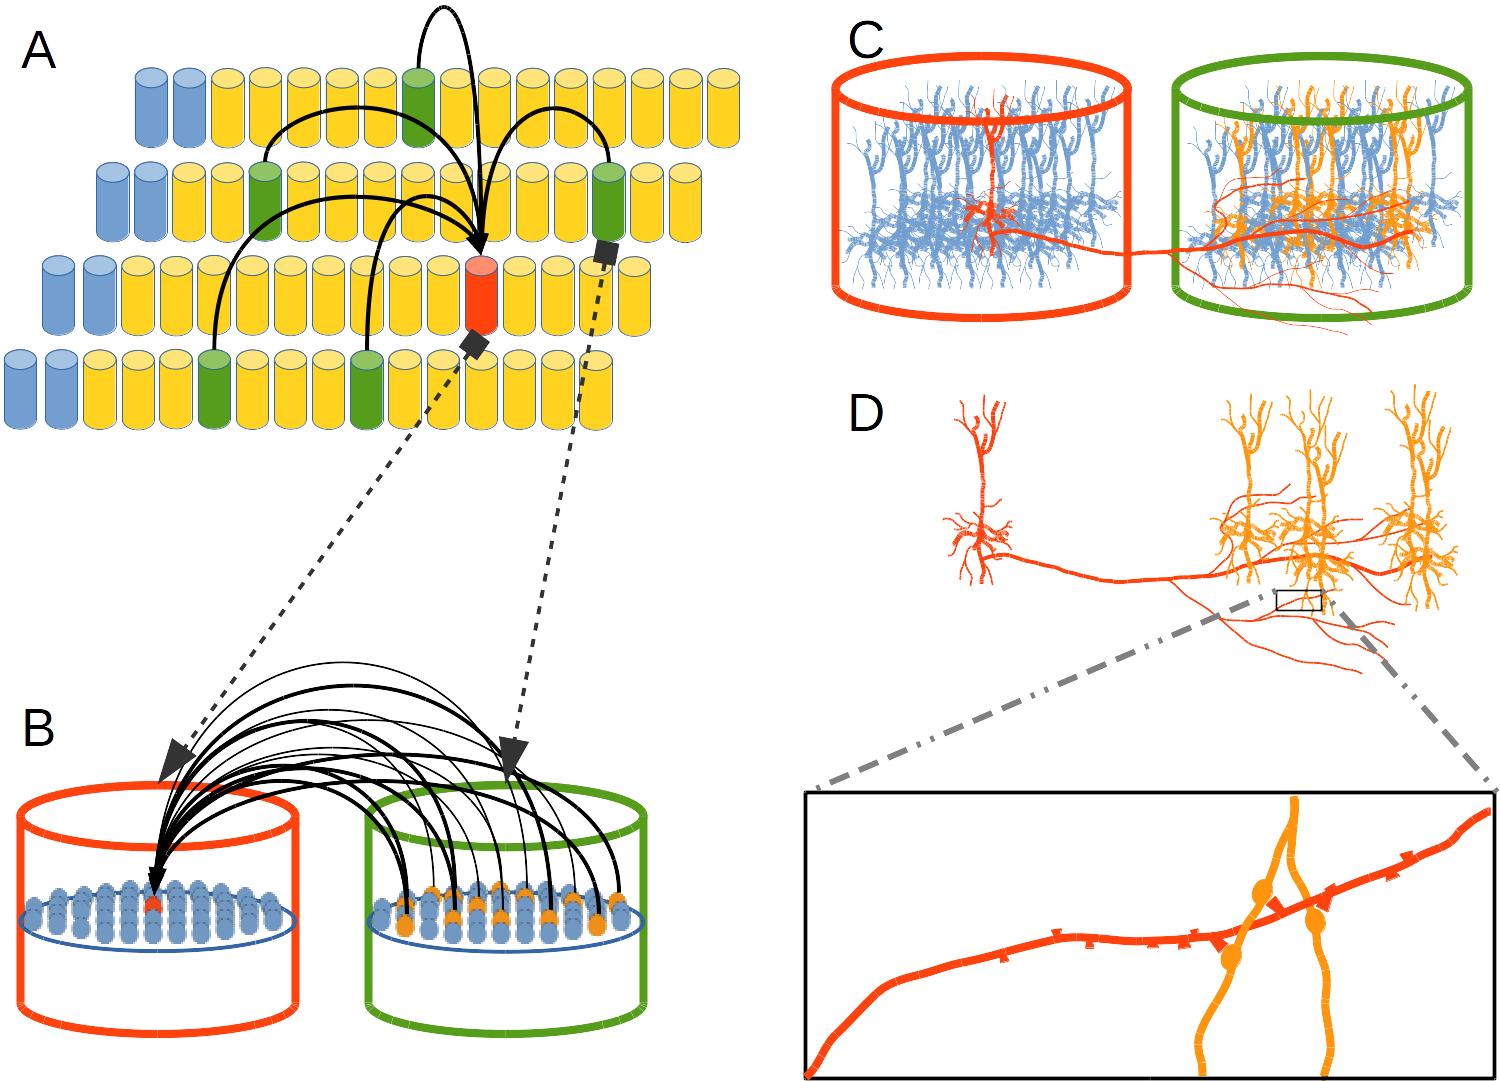
\includegraphics[width=0.9\textwidth]{DistalDendrites.png}
    \caption{Conexiones dendríticas distales. (A) Ramas dendríticas distales desde \glspl{cc} vecinas dentro del campo receptivo
	    de una \gls{cc} en la \gls{el}. Una rama dendrítica distal entre la \gls{cc} roja y una
	    \gls{cc} verde significa que cada unidad neuronal en la \gls{cc} roja está vinculada con un subconjunto diferente
	    de unidades neuronales en la \gls{cc} verde por medio de conexiones potenciales.
	    (B) Conexiones potenciales en una rama dendrítica que vincula una unidad neuronal en la \gls{cc} roja
	    con un subconjunto de unidades neuronales en una \gls{cc} verde. El subconjunto de conexiones potenciales viene de un porcentaje de unidades neuronales
	    dentro de una \gls{cc} verde. Tal porcentaje es un parámetro ajustable para la \gls{cc}.
	    (C) Una rama dendrítica distal entre una célula piramidal en una \gls{cc} y un
	    subconjunto de células piramidales en una \gls{cc} vecina dentro de su campo receptivo en la \gls{el}.
	    (D) Proximidad física de una rama dendrítica desde la célula roja a las ramas axonales desde las células amarillas constituyen conexiones potenciales
	    que pueden prosperar convirtiéndose en sinapsis establecidas dependiendo de la actividad secuencial entre las células.}
    \label{fig:DistalDendrites}
\end{figure}

Tales vínculos en la Fig \ref{fig:DistalDendrites} A, representan ramas dendríticas en el tejido neuronal.
Llamamos a cada conexión en la Fig. \ref{fig:DistalDendrites} B, conexión potencial.
Las conexiones potenciales representan sinapsis en la rama dendrítica.
Una unidad celular dentro de la \gls{cc} roja termina con tantas ramas dendríticas como \glspl{cc} verdes dentro de su campo receptivo (Fig \ref{fig:DistalDendrites} A.)

El término \emph{conexión potencial} es usado, porque describe un par de unidades neuronales vinculadas por sus ubicaciones físicas y disposición dendrítica y axonal en el tejido cortical (Fig. \ref{fig:DistalDendrites} C). Sin embargo, la conectividad efectiva entre tales neuronas dependerá de su patrón secuencial de activación el cual establecerá sinapsis desarrolladas entre ellas. 
Si dos unidades neuronales--una roja y una amarilla en la Fig. \ref{fig:DistalDendrites} D--se vinculan por medio de una conexión potencial distal--producida por una sinapsis entre una rama dendrítica distal desde la roja y una rama axonal desde la amarilla--tal conexión crecerá solo si existe una activación secuencial de la célula roja después de una activación de la célula amarilla, en dos pasos temporales consecutivos.
Si tal fenómeno no se repite en el tiempo, tal sinapsis decrementará su fuerza con respecto a otras sinapsis en la rama dendrítica en la célula roja en la Fig. \ref{fig:DistalDendrites} D.
Una activación simultánea en ambas unidades neuronales--la roja y la amarilla en la Fig. \ref{fig:DistalDendrites} D--decrementará la sinapsis en tal conexión potencial.

Implementamos mecanismos de plasticidad sinaptica en dendritas distales por medio de un algoritmo llamado \gls{dsom} (Alg. \ref{csom_distal_synapses}).
Los mecanismos de aprendizaje implementados en tal algoritmo simulan fenómenos neurofisiológicos
tales como \gls{stdp}, y plasticidad de regulación homeostática en la determinación del peso sinaptico en las ramas dendríticas distales.

\begin{algorithm}
	\caption{\texttt{Plasticity in Distal Synapses}. This algorithm accounts for \glsfirst{stdp} and homeostatic regulation phenomenon in distal dendritic synapses.}
\label{csom_distal_synapses}
\begin{algorithmic}[1]
	\FOR{every active \texttt{unit} in this cortical \texttt{column}}
		\FOR{every \texttt{dendrite} in this active \texttt{unit}}
			\STATE {increment all the \texttt{synapses}--in this dendrite--potentially connected to \texttt{units} which were active in the last time step}
		\ENDFOR
	\ENDFOR
	\FOR{every active \texttt{unit} in this cortical \texttt{column}}
		\FOR{every \texttt{dendrite} in this active \texttt{unit}}
			\STATE {decrement all the \texttt{synapses}--in this dendrite--potentially connected to \texttt{units} which are active in this time step}
		\ENDFOR
	\ENDFOR
	\IF{updated \texttt{step} reaches certain value}
		\FOR{every \texttt{unit} in this cortical \texttt{column}}
			\FOR{every \texttt{dendrite} in this \texttt{unit}}
				\IF{the sum of the \texttt{synapses} in this \texttt{dendrite} is greater than one}
					\STATE {normalize all \texttt{synapses} in this \texttt{dendrite}}
				\ENDIF
			\ENDFOR
		\ENDFOR
		\STATE{updated \texttt{step} = 0}
	\ENDIF
	\STATE{updated \texttt{step}++} 
\end{algorithmic}
\end{algorithm}

Básicamente, el Alg.~\ref{csom_distal_synapses} actualiza todas las sinapsis axo-dendríticas distales, incrementándolas siempre que unidades neuronales pre y post-sinapticas se activan en pasos temporales consecutivos, y las decrementa cuando se activan en el mismo paso temporal. Ocasionalmente, todos los pesos sinapticos pertenecientes a la misma dendrita se normalizan cada cierto número de pasos temporales. Esta normalización se repite para todas las unidades neuronales y para todas las ramas dendríticas en cada unidad neuronal cuya suma de sus pesos sinapticos excede la unidad.
}{
In terms of distal dendritic branches, each \gls{cc} in the \gls{el} is connected to other \glspl{cc}--in green in Fig \ref{fig:EncoderColumnConnections}--by means of such
branches inside the receptive fields--in yellow in Fig. \ref{fig:EncoderColumnConnections}--from the same \gls{el} and from another \gls{cl}
above.
Each link between the red \gls{cc} and a green \gls{cc}--Fig. \ref{fig:DistalDendrites} A--
symbolizes the fact that each cell unit in
the red \gls{cc} is linked with a different subset of cell units in the green \gls{cc}--Fig. \ref{fig:DistalDendrites} B.

\begin{figure}[h!]
    \centering
    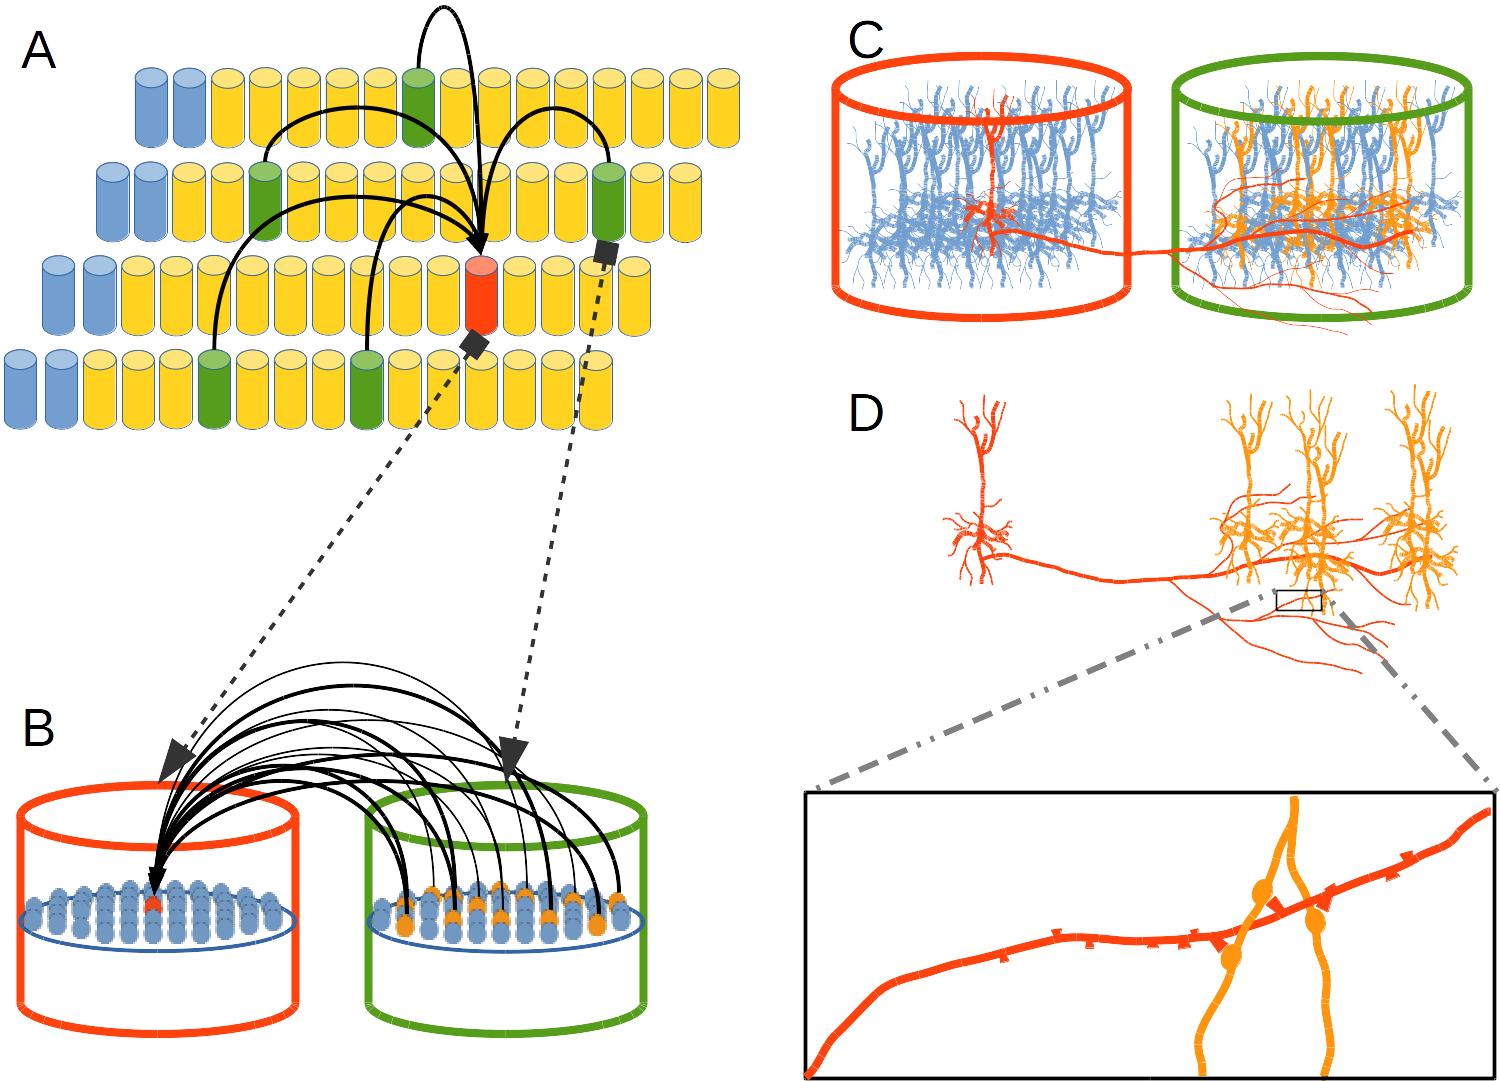
\includegraphics[width=0.9\textwidth]{DistalDendrites.png}
    \caption{Distal dendrite connections. (A) Distal dendritic branches from neighboring \glspl{cc} inside the receptive field
    of a \gls{cc} in the \gls{el}. A distal dendritic branch between the red \gls{cc} and a
    green \gls{cc} means that every neural unit in the red \gls{cc} is linked with a different
    subset of neural units in the green \gls{cc} by means of potential connections.
    (B) Potential connections in a dendritic branch which link a neural unit in the red \gls{cc}
    with a subset of neural units in a green \gls{cc}. The subset of potential connections comes from a percentage of neural units
    inside the green \gls{cc}. Such percentage is a tunable parameter for the \gls{cc}.
    (C) A distal dendritic branch between a pyramidal cell in a \gls{cc} and a 
    sub-set of pyramidal cells in a neighboring \gls{cc} inside its receptive field
    in the \gls{el}.
    (D) Physical proximity of a dendritic branch from the red cell to axonal branches from yellow cells constitutes potential connections
    which could prosper becoming in established synapses depending on the sequential activity among cells.}
    \label{fig:DistalDendrites}
\end{figure}

Such links in Fig \ref{fig:DistalDendrites} A, represent dendritic branches in neural tissue and
we call
each connection in Fig. \ref{fig:DistalDendrites} B,
potential connection.
Potential connections represent synapses in the dendritic branch.
A cell unit inside the red \gls{cc} ends up with as many dendritic branches as green \glspl{cc} inside its receptive field (Fig \ref{fig:DistalDendrites} A.)

The term \emph{potential connection} is used, because it describes a pair of neural units linked by its physical location and dendritic and axonal disposition in cortical tissue (Fig. \ref{fig:DistalDendrites} C). However, an effective connectivity between such neurons will depend upon their sequential pattern of activation which will establish developed synapses between them. If two neural units--a red one and a yellow one in Fig. \ref{fig:DistalDendrites} D--are linked by means of a distal potential connection--produced by a synapse between a distal dendritic branch from the red one and an axonal branch from the yellow one--such connection will grow only if there is a sequential activation of the red cell after an activation of the yellow cell, in two consecutive time steps. If such phenomenon does not repeat itself over time, such synapse will decrease its strength with respect to other synapses in the dendritic branch in the red cell in Fig. \ref{fig:DistalDendrites} D. A simultaneous activation in both neural units--the red one and the yellow one in Fig. \ref{fig:DistalDendrites} D--will decrease the strength in such potential connection.

We implemented distal dendritic synaptic plasticity mechanisms by means of an algorithm called \gls{dsom} (Alg. \ref{csom_distal_synapses}).
The learning mechanisms implemented on such algorithm simulate neurophysiological phenomena
such as \gls{stdp}, and homeostatic regulation plasticity in the synaptic strength regulation in
distal dendritic branches.

\begin{algorithm}
	\caption{\texttt{Plasticity in Distal Synapses}. This algorithm accounts for \glsfirst{stdp} and homeostatic regulation phenomenon in distal dendritic synapses.}
\label{csom_distal_synapses}
\begin{algorithmic}[1]
	\FOR{every active \texttt{unit} in this cortical \texttt{column}}
		\FOR{every \texttt{dendrite} in this active \texttt{unit}}
			\STATE {increment all the \texttt{synapses}--in this dendrite--potentially connected to \texttt{units} which were active in the last time step}
		\ENDFOR
	\ENDFOR
	\FOR{every active \texttt{unit} in this cortical \texttt{column}}
		\FOR{every \texttt{dendrite} in this active \texttt{unit}}
			\STATE {decrement all the \texttt{synapses}--in this dendrite--potentially connected to \texttt{units} which are active in this time step}
		\ENDFOR
	\ENDFOR
	\IF{updated \texttt{step} reaches certain value}
		\FOR{every \texttt{unit} in this cortical \texttt{column}}
			\FOR{every \texttt{dendrite} in this \texttt{unit}}
				\IF{the sum of the \texttt{synapses} in this \texttt{dendrite} is greater than one}
					\STATE {normalize all \texttt{synapses} in this \texttt{dendrite}}
				\ENDIF
			\ENDFOR
		\ENDFOR
		\STATE{updated \texttt{step} = 0}
	\ENDIF
	\STATE{updated \texttt{step}++} 
\end{algorithmic}
\end{algorithm}

Basically, Alg.~\ref{csom_distal_synapses} updates all distal axonal-dendritic synapses, incrementing  them always that pre and post-synaptic neural units become active in consecutive time steps, and decrementing them when they become active at the same time step. Occasionally, all the synaptic weights belonging to the same dendrite are normalized every certain number of time steps. This normalization is repeated for all neural units and for all dendritic branches in each neural unit whose sum of synaptic weights is beyond unity.
}
























%\subsubsection{Reglas de Activación en una Columna Cortical}


\iftoggle{DEBUG}{
Finalmente, en referencia a las reglas de activación de las unidades neuronales dentro de una \gls{cc} en la \gls{el},
primero un grupo de unidades celulares en una \gls{cc} es depolarizada parcialmente
por las conexiones distales entre tales unidades neuronales y unidades celulares activadas en el
paso temporal previo en la \gls{el}--Fig. \ref{fig:Activation} A.
Es decir, las unidades neuronales activadas en el paso temporal $t=0$ en la \gls{el}, depolarizarán parcialmente
un conjunto de unidades neuronales en el paso temporal $t=1$ en tal \gls{cc}, por medio de sinapsis en ramas dendríticas distales--laterales y apicales--
establecidas por el algoritmo \gls{dsom}.

Segundo, las conexiones próximas aferentes desde el \gls{mrstsa} tenderán a depolarizar
ciertos cúmulos de unidades en tal \gls{cc} en el paso temporal $t=1$--Fig. \ref{fig:Activation} B.
La depolarización tentativa es producida por las entradas desde el \gls{mrstsa} con
las sinapsis próximas establecidas por el algoritmo \gls{ssom}.
Tal grupo de unidades neuronales son escojidas aleatoriamente desde una distribución discreta
cuyas probabilidades se establecen por el estado de excitación en las entradas aferentes.

Si un número suficientemente grande de unidades parcialmente depolarizadas se encuentra en el conjunto de
unidades exitadas aferentemente, tales unidades parcialmente depolarizadas
dispararán antes en el grupo--Fig. \ref{fig:Activation} B izquierda.
Esas unidades--las cuales disparan antes--evitan que unidades vecinas en los cúmulos excitados disparen,
sobrepolarizandolas por medio de conexiones inhibitorias laterales en la columna.

\begin{figure}[h!]
    \centering
    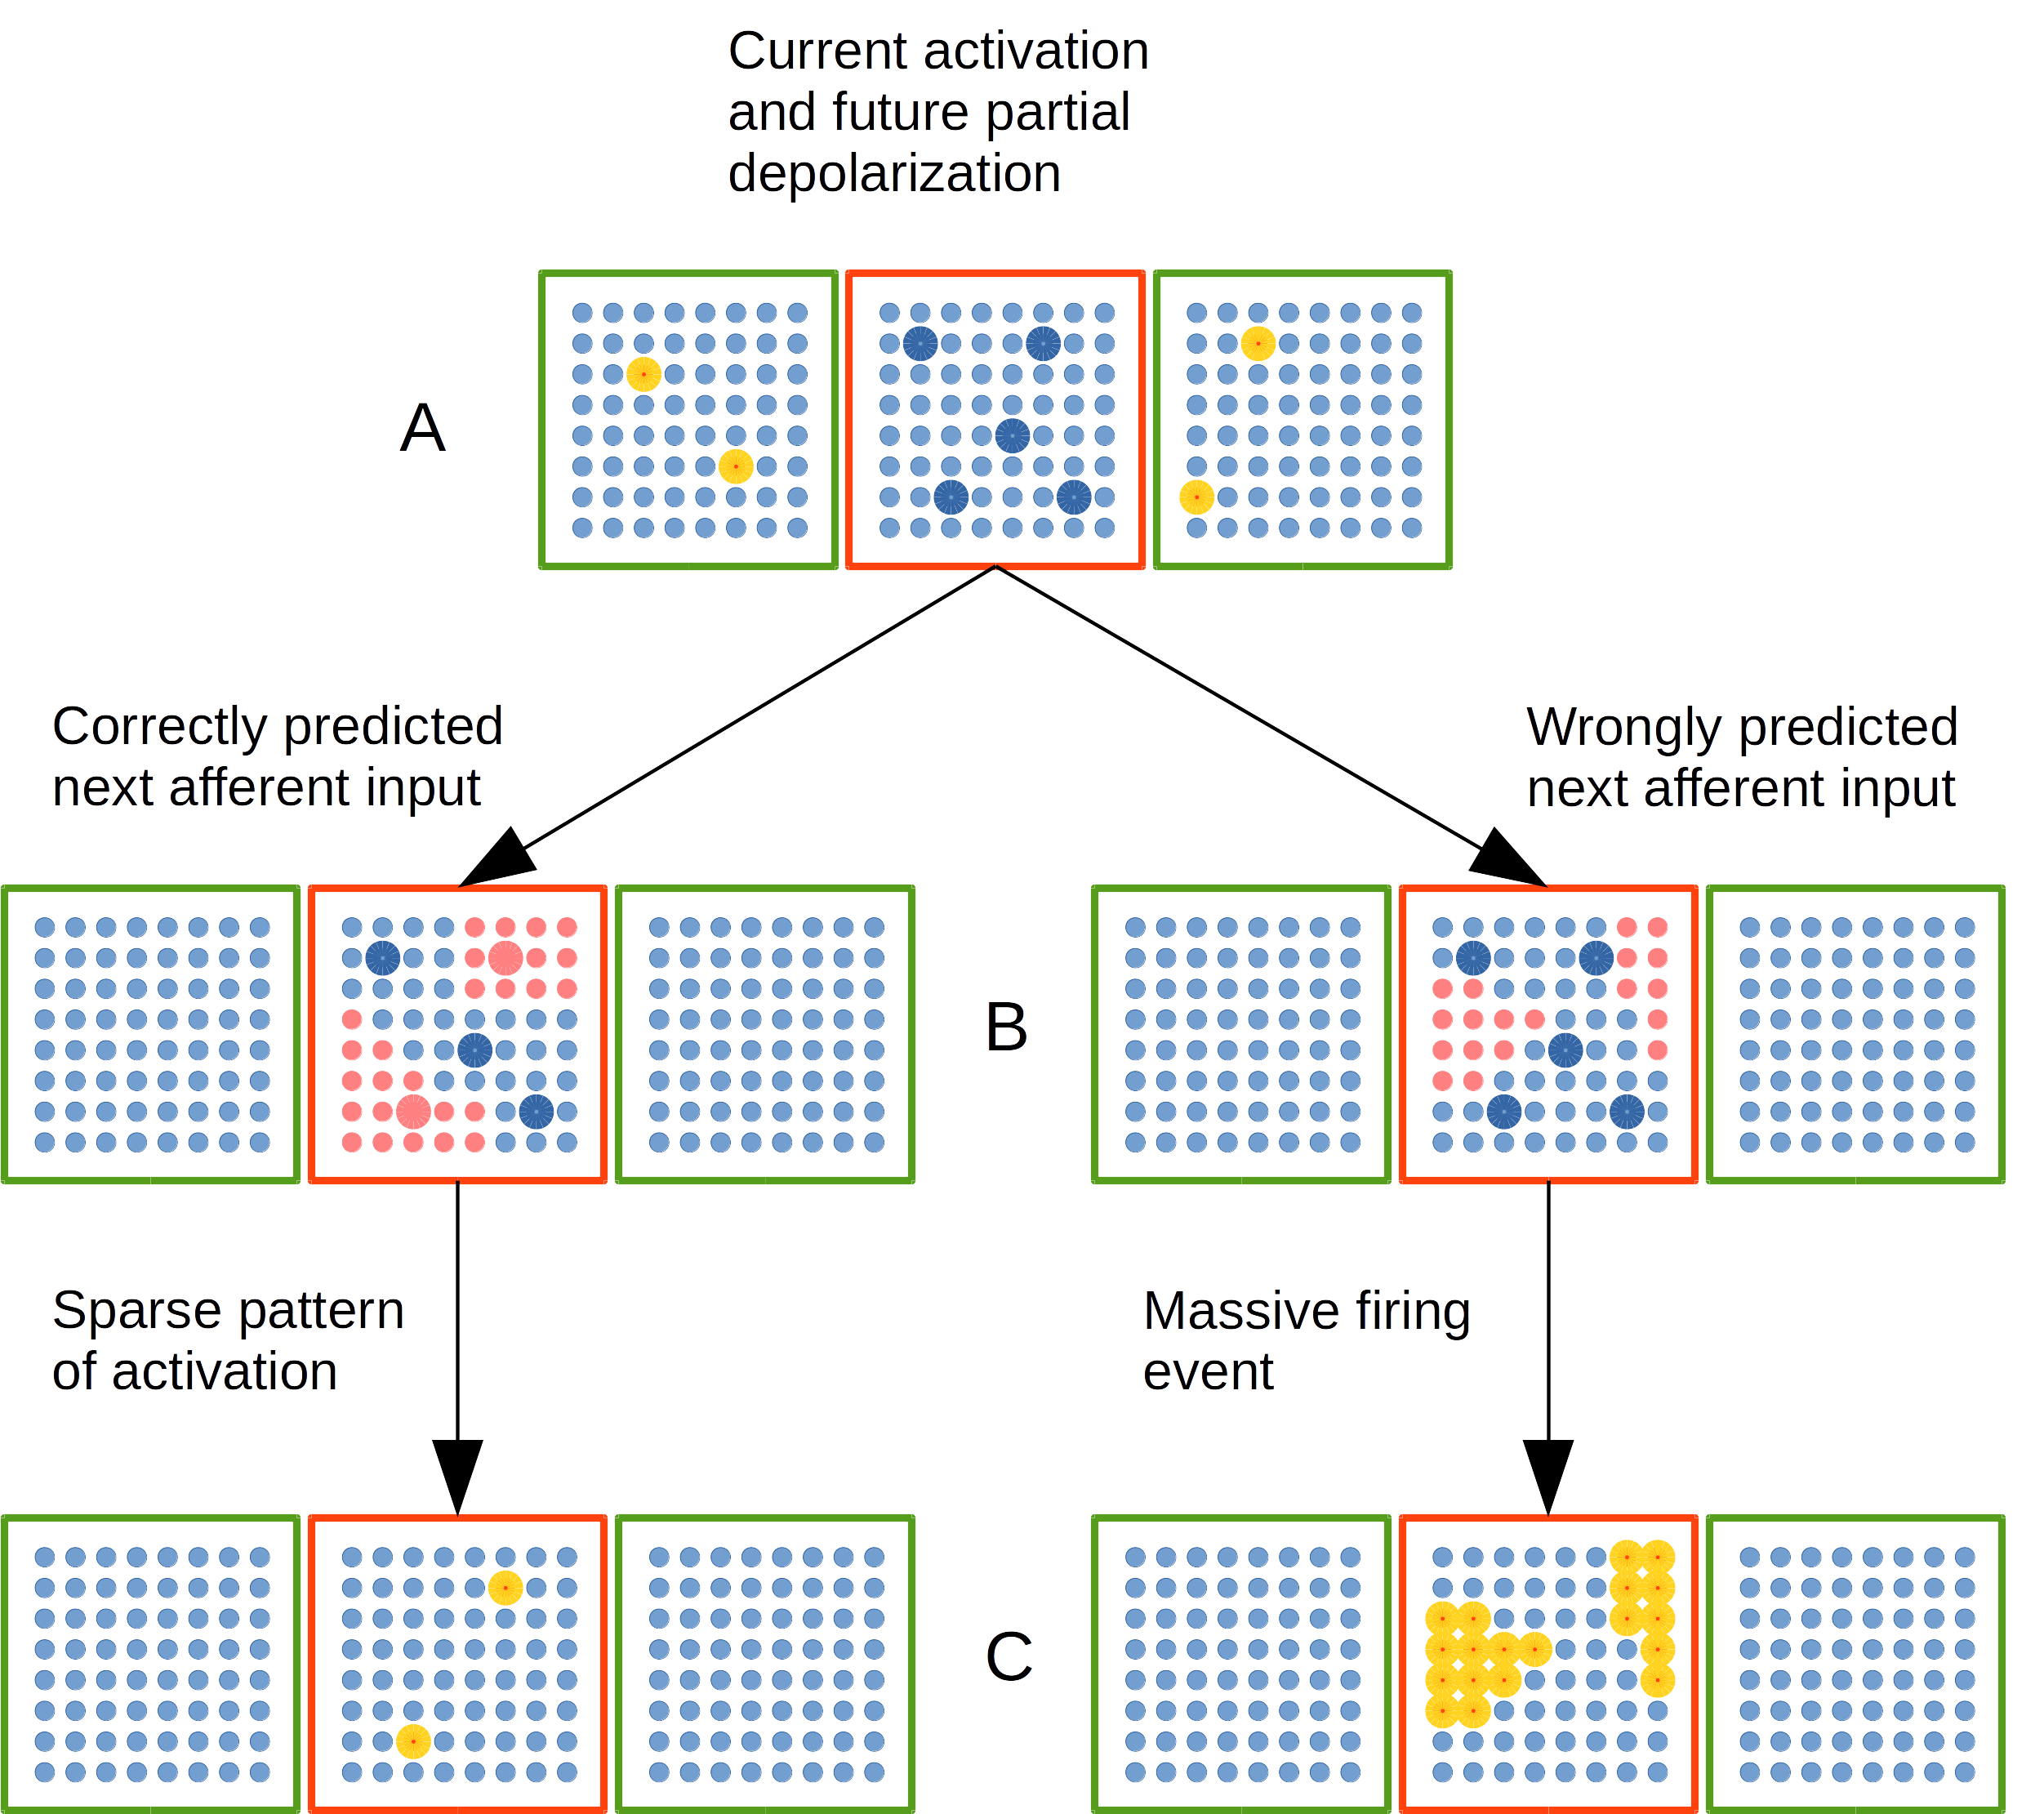
\includegraphics[width=0.7\textwidth]{Activation.png}
    \caption{Activación celular dinámica en una \gls{cc} en la \gls{el}.
	    Una columna cortical roja está vinculada con dos columnas corticales por medio de dendritas distales.
	    (A) Activación celular en las \glspl{cc} verdes--resaltadas en las células amarillas--ponen las unidades neuronales
	    en la \gls{cc} roja en un estado de depolarización parcial--predictivo resaltado en azul.
	    (B) Cúmulo de células neuronales activadas por entrads aferentes.
	    Izquierda: Una cantidad sustancial de células depolarizadas parcialmente está dentro de los cúmulos celulares activados aferentemente.
	    Derecha: No hay una cantidad sustancial de células depolarizadas parcialmente dentro de los cúmulos celulares excitados aferentemente.
	    (C) \gls{cc} con unidades celulares activas resaltadas en amarillo.
	    Izquierda: Activación celular de patrón disperso.
	    Derecha: Activación de patrón masivo.}
    \label{fig:Activation}
\end{figure}

Los estados de depolarización parcial ponen a las unidades celulares en un estado predictivo por
la activación producida en la \gls{el} en pasos temporales previos.
Es decir, la cativación lateral y apical en pasos temporales previos constituye un contexto en el cual
las entradas aferentes actuales son recibidas.

Del grupo de unidades que tienden a ser depolarizadas por las entradas aferentes desde el \gls{mrstsa},
solo un subconjunto reducido pueden disparar dada la historia de activaciones contextuales previas
en la  \gls{el}--Fig. \ref{fig:Activation} C izquierda.

En caso de no haber contexto, es decir, si no hay suficientes unidades que están parcialmente depolarizadas 
por activaciones--laterales y apicales--previas--Fig. \ref{fig:Activation} B derecha--,
dentro del conjunto de unidades
normalmente depolarizadas por entradas aferentes,
todas las unidades en los cúmulos excitados aferentemente se activarán, cubriendo más hipótesis para las siguientes entradas--Fig. \ref{fig:Activation} C derecha.

Tal mecanismo de activación es delineado en el Alg. \ref{csom_activation}. En el Alg. \ref{csom_activation} (Parte 1) se establece un ranking entre unidades neuronales--dentro de una \gls{cc}--en términos de su excitabilidad aferente, dadas las entradas aferentes (líneas 1 y 2).
El parámetro \emph{number of afferently excited units} se refienre al máximo número de unidades que pueden ser activadas por la entrada aferente en una \gls{cc} y \emph{minimum number of active units} se refiere al número de unidades que serán activadas en una \gls{cc} si una \gls{sdr} se alcanza como resultado de una predicción óptima (líneas 3 y 4 respectivamente).

\begin{algorithm}
	\caption{\texttt{Units activation (Part 1)}. This algorithm establishes the activation rules in a \gls{csom} object.}
\label{csom_activation}
\begin{algorithmic}[1]
	\STATE{\texttt{distances} = given an \texttt{input} vector find the euclidean distance each \texttt{unit} has to such \texttt{input} in the input space from proximal afferent synapses}

	\STATE {\texttt{ranking} = sort indexes from the smallest to the largest \texttt{distances}}

	\STATE{number of afferently excited units = proximal activation percentage*number of units}

	\STATE{minimum number of active units = (1-sparsity)*number of units}

	\IF{randomness is disabled}
		\STATE {excited \texttt{units} = gets the first \emph{number of afferently excited units} elements from \texttt{ranking}}
	\ELSE
		\STATE {excited \texttt{units} = gets \emph{number of afferently excited units} random indexes from \texttt{distances} with probabilities determined by the relative reciprocal of the \texttt{distances} element values}
	\ENDIF

	\FOR{\texttt{unit} = 0 \TO \texttt{unit} = number of units }
		\STATE{auxiliary = 0}
		\FOR{\texttt{dendrite} = 0 \TO \texttt{dendrite} = number of distal dendrites }
			\STATE{\texttt{dendrite} accumulator = 0}
			\FOR{\texttt{active unit} = 0 \TO \texttt{active unit} = number of linked active units}
				\STATE{potential \texttt{index} = find the first coincident index in potential \texttt{connections[dendrite][unit]} with linking \texttt{units[dendrite][active unit]}}
				\IF{there exist coincidence}
					\STATE {\texttt{dendrite} accumulator += dynamic \texttt{synapses[dendrite][unit][\textnormal{potential} index]}}
				\ENDIF
			\ENDFOR
			\IF{\texttt{dendrite} accumulator $>$ 100*DISTAL\_SYNAPTIC\_THRESHOLD}
				\STATE {auxiliary++}
			\ENDIF
		\ENDFOR
		\STATE{total \texttt{responses[unit]} += auxiliary}
	\ENDFOR
	\STATE{updated \texttt{distances} = element wise quotient between \texttt{distances} and total \texttt{responses}}
	\STATE {updated \texttt{ranking} = sort indexes from the smallest to the largest updated \texttt{distances}}

\end{algorithmic}
\end{algorithm}

Si la aleatoriedad está habilitada, se escogen \emph{number of afferently excited units} unidades aleatoriamente por medio de una distribución discreta cuyas probabilidades son la excitación aferente de cada unidad. Si la aleatoriedad está deshabilitada, las \emph{number of afferently excited units} primeras unidades son escogidas desde un ranking de unidades excitadas aferentemente (líneas 5 a 9).

Desde la línea 10 a la 25 cada unidad neuronal acumula excitación--lateral y apical--distal para determinar su depolarización parcial desde las unidades que estuvieron activas en el paso temporal previo. Para cada unidad neuronal en una \gls{cc}, para cada dendrita distante en tal unidad y para cada unidad activa en tal dendrita distante el algoritmo busca coincidencias entre algunas conexiones potenciales en tal dendrita distal en la unidad neuronal y la unidad activa en tal dendrita distal.
Es decir, en la línea 15, el algoritmo pregunta se hay coincidencia entre algunas conexiones potenciales en esta dendrita distante dentro de la unidad y las unidades neuronales activadas en el paso temporal previo en la \gls{cc} vinculada por tal dendrita.
Si hay coincidencia, el valor del peso sinaptico en tal conexión potencial es acumulado en un acumulador de la dendrita.
Después de que todas las unidades activas son examinadas por esta dendrita, si el acumulador de la dendrita es mayor que cierto umbral, tal dendrita es considerada activa y la respuesta total de la unidad se incrementa en uno.

Cada unidad neuronal termina con un valor de excitación debido a sus dendritas distales. El vector de distancias de la unidad es dividido componente por componente por el vector de excitaciones dendríticas para obtener distancias actualizadas y un ranking actualizado de las unidades (líneas 26 y 27). De esta manera, las unidades con más excitación distal decrementarán sus distancias más, y serán puestas en un lugar más favorable en el ranking para ser activadas.

En el Alg. \ref{csom_activation} (Parte 2) la distancia actualizada mínima es hallada en el grupo de unidades excitadas aferentemente. Luego, un conjunto de unidades con tal distancia mínima--dentro de dicho grupo--es identificado. Mientras el número de unidades identificadas sea menor que \emph{minimum number of active units}, se halla la siguiente distancia actualizada mínima en el grupo de unidades excitadas aferentemente y un nuevo conjunto de unidades--dentro de dicho grupo--es identificado. Dichas unidades tienen tal distancia actualizada mínima siguiente.
Este nuevo conjunto es sumado al conjunto previo hasta que el número de unidades en el conjunto acumulativo es mayor o igual que el mínimo número de unidades activas.

\begin{algorithm}
\ContinuedFloat
\caption{\texttt{Units activation (Part 2)}. This algorithm establishes the activation rules in a \gls{csom} object.}
\label{csom_activation}
\begin{algorithmic}[1]
	\STATE{new \texttt{distances} = get the updated \texttt{distances} elements whose indexes are in excited \texttt{units}}
	\STATE{new minimum \texttt{distance} = get the minimum element from new \texttt{distances}}
	\STATE{minimum \texttt{indexes} = get indexes from updated \texttt{distances} vector whose values are equal to new minimum \texttt{distance}}
	\STATE{apt to be \texttt{active} = get the coincident indexes between excited \texttt{units} and minimum \texttt{indexes}}
	\STATE{erase from new \texttt{distances} vector, all the elements whose value is equal to new minimum \texttt{distance}}

	\WHILE{number of elements in apt to be \texttt{active} vector $<$ \emph{minimum number of active units} and new \texttt{distances} has at least one element}
		\STATE{new minimum \texttt{distance} = get the minimum element from new \texttt{distances}}
		\STATE{minimum \texttt{indexes} = get indexes from updated \texttt{distances} vector whose values are equal to new minimum \texttt{distances}}
		\STATE{partial apt to be \texttt{active} = get the coincident indexes between excited \texttt{units} and minimum \texttt{indexes}}
		\STATE{incorporate partial apt to be \texttt{active} elements into apt to be \texttt{active} vector}
		\STATE{erase from new \texttt{distances} vector, all the elements whose value is equal to new minimum \texttt{distance}}
	\ENDWHILE

	\IF{ENABLE\_RANDOM\_BEHAVIOUR}
		\STATE {shuffle apt to be \texttt{active} vector}
	\ENDIF

	\FOR{\texttt{number} = 0 \TO \texttt{number} = number of apt to be \texttt{active} elements }
		\STATE {incorporate to \texttt{output} the excited \texttt{units[\textnormal{apt to be} active[number]]}}
	\ENDFOR

	\RETURN \texttt{output}
\end{algorithmic}
\end{algorithm}

El resultado funcional del Alg. \ref{csom_activation} es que debe haber una cantidad suficiente de unidades neuronales--parcialmente y previamente depolarizadas--dentro del cúmulo de unidades aferentemente activadas para conseguir un patrón de activación \gls{sdr}. De otra forma, la \gls{cc} terminará con un patrón de activación masiva, un \glsfirst{mfe} en el cual más que \emph{minimum number of active units} unidades serán activadas.
En el caso de la ocurrencia de un \gls{mfe}, la plasticidad sinaptica es modulada para formar sinapsis más fuertes de las unidades neuronales activadas durante tal evento.

Cada unidad neuronal en una \gls{cc} establece su estado de depolarización parcial basado en la contribución desde
las ramas dendríticas distales desde conexiones laterales y apicales.
Una rama dendrítica contribuirá a la depolarización parcial del soma en tal célula solo si tal
rama dendrítica excede un umbral deactivación por medio de la contribución de sus sinapsis individuales
en el contexto de los patrones de activación en el paso temporal previo.

Este mecanismo posee propiedades secuenciales convincentes \cite{hawkins_2016},
que ya han sido aplicadas a la clasificación de datos secuenciales generados artificialmente \cite{cui_2016}.
Aplicamos tales mecanismos en el algoritmo \gls{dsom} por medio de la adición de la contribución de sinapsis--en una rama dendrítica--cuyas conexiones
son vinculadas con células que fueron activadas en los pasos temporales previos en la \gls{el}.
}{
Finally, in reference to the activation rules of neural units inside a \gls{cc} in the \gls{el},
first a group of cell units in a \gls{cc} is partially depolarized 
by distal connections among such neural units and cell units activated in the
previous time step in the \gls{el}--Fig. \ref{fig:Activation} A.
That is, neural units activated in time step $t=0$ in the \gls{el}, will partially depolarize
a set of neural units in time step $t=1$ in such \gls{cc}, by means of distal--lateral and apical--
dendritic branch synapses established by learning in the \gls{dsom} algorithm.

Second, afferent proximal connections from \gls{mrstsa} will tend to depolarize
certain clusters of units in such \gls{cc} in time step $t=1$--Fig. \ref{fig:Activation} B.
The tentative depolarization is produced by the inputs from the \gls{mrstsa} with
proximal synapses established by learning in the \gls{ssom} algorithm. 
Such group of neural units are randomly chosen from a discrete distribution
whose probabilities are established by the state of excitation in afferent inputs.

If a sufficient number of partially depolarized units are in the set of
afferently excited units, such partially depolarized units
will fire previously in the group--Fig. \ref{fig:Activation} B left.
Those units--which fire before--prevent neighboring units in the excited clusters from firing,
hyperpolarizing them by means of lateral inhibitory connections in the column.

\begin{figure}[h!]
    \centering
    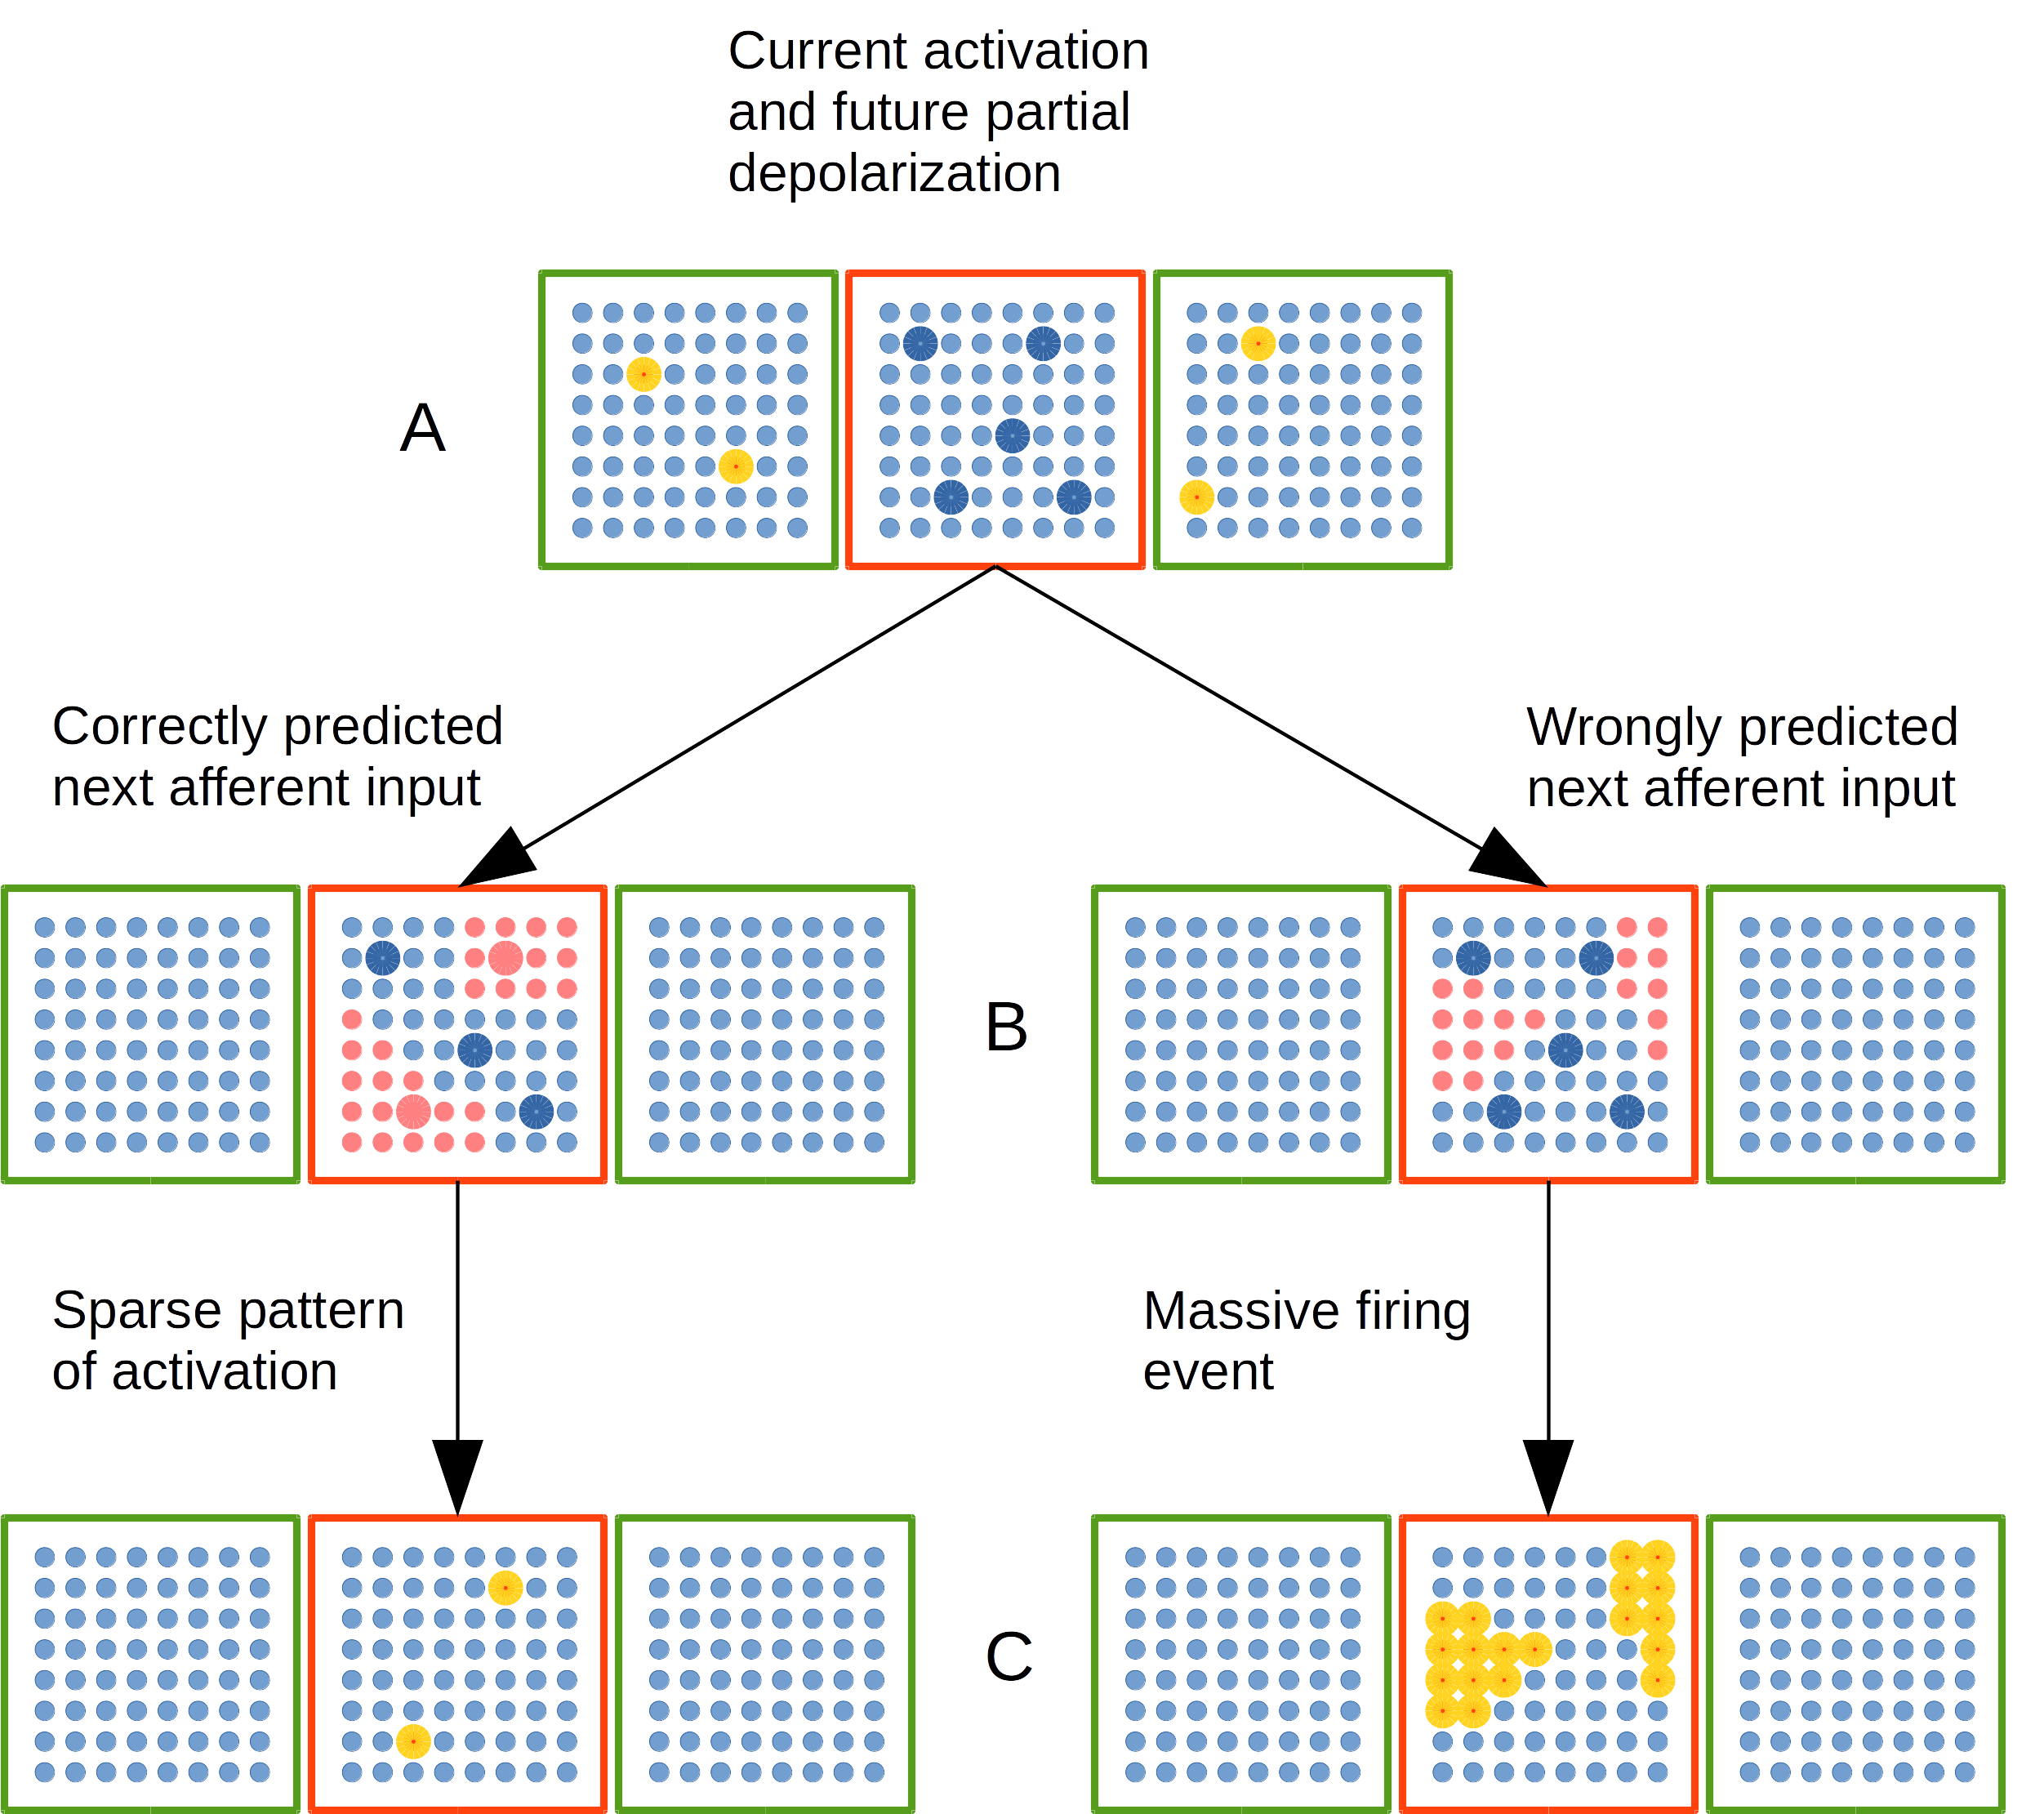
\includegraphics[width=0.7\textwidth]{Activation.png}
    \caption{Dynamic cellular activation in a \gls{cc} in the \gls{el}.
    A red cortical column is linked with two green cortical columns by means of distal dendrites.
    (A) Cellular activation in green \glspl{cc}--highlighted yellow cells--puts neural units
    in red \gls{cc} in a partially depolarized--predictive state highlighted in blue.
    (B) Cluster of neural cells activated by afferent inputs.
    Left: A substantial amount of partially depolarized cells are in the afferently excited cellular clusters.
    Right: There is no substantial amount of partially depolarized cells inside afferently excited cellular clusters.
    (C) \gls{cc} with active cellular units highlighted in yellow.
    Left: Sparse pattern of cellular activation.
    Right: Massive pattern of activation.}
    \label{fig:Activation}
\end{figure}

Partial depolarization states put cell units in a predictive state generated by
the activations produced in the \gls{el} in previous time steps.
That is, lateral and apical activation in previous time steps constitute a context in which
current afferent inputs are received.

From the group of units that tend to be depolarized by current afferent inputs from the \gls{mrstsa},
only a reduced sub-set of those units are likely to fire in the previous contextual firing history
in the \gls{el}--Fig. \ref{fig:Activation} C left.

In case there is no context, that is, if not enough units normally depolarized by afferent inputs
are partially depolarized by previous--lateral and apical--activations--Fig. \ref{fig:Activation} B right--,
all units in the afferent excited clusters will be active, covering more hypotheses for next inputs--Fig. \ref{fig:Activation} C right.

Such activation mechanism is depicted in Alg. \ref{csom_activation}. In Alg. \ref{csom_activation} (Part 1) a ranking is established among neural units--inside a \gls{cc}--in terms of its afferent excitability, given the afferent inputs (lines 1 and 2). The \emph{number of afferently excited units}  refers to the maximum number of  units that can be activated by the afferent input in a \gls{cc} and \emph{minimum number of active units} refers to the number of units that will be active in a \gls{cc} if a \gls{sdr} is achieved as a result of optimal prediction (lines 3 and 4 respectively).

\begin{algorithm}
	\caption{\texttt{Units activation (Part 1)}. This algorithm establishes the activation rules in a \gls{csom} object.}
\label{csom_activation}
\begin{algorithmic}[1]
	\STATE{\texttt{distances} = given an \texttt{input} vector find the euclidean distance each \texttt{unit} has to such \texttt{input} in the input space from proximal afferent synapses}

	\STATE {\texttt{ranking} = sort indexes from the smallest to the largest \texttt{distances}}

	\STATE{number of afferently excited units = proximal activation percentage*number of units}

	\STATE{minimum number of active units = (1-sparsity)*number of units}

	\IF{randomness is disabled}
		\STATE {excited \texttt{units} = gets the first \emph{number of afferently excited units} elements from \texttt{ranking}}
	\ELSE
		\STATE {excited \texttt{units} = gets \emph{number of afferently excited units} random indexes from \texttt{distances} with probabilities determined by the relative reciprocal of the \texttt{distances} element values}
	\ENDIF

	\FOR{\texttt{unit} = 0 \TO \texttt{unit} = number of units }
		\STATE{auxiliary = 0}
		\FOR{\texttt{dendrite} = 0 \TO \texttt{dendrite} = number of distal dendrites }
			\STATE{\texttt{dendrite} accumulator = 0}
			\FOR{\texttt{active unit} = 0 \TO \texttt{active unit} = number of linked active units}
				\STATE{potential \texttt{index} = find the first coincident index in potential \texttt{connections[dendrite][unit]} with linking \texttt{units[dendrite][active unit]}}
				\IF{there exist coincidence}
					\STATE {\texttt{dendrite} accumulator += dynamic \texttt{synapses[dendrite][unit][\textnormal{potential} index]}}
				\ENDIF
			\ENDFOR
			\IF{\texttt{dendrite} accumulator $>$ 100*DISTAL\_SYNAPTIC\_THRESHOLD}
				\STATE {auxiliary++}
			\ENDIF
		\ENDFOR
		\STATE{total \texttt{responses[unit]} += auxiliary}
	\ENDFOR
	\STATE{updated \texttt{distances} = element wise quotient between \texttt{distances} and total \texttt{responses}}
	\STATE {updated \texttt{ranking} = sort indexes from the smallest to the largest updated \texttt{distances}}

\end{algorithmic}
\end{algorithm}

If randomness is enabled, \emph{number of afferently excited units} units is chosen at random by means of a discrete distribution whose probabilities are the afferent excitation of each unit. If randomness is disabled, \emph{number of afferently excited units} first units are chosen from the ranking of afferently excited units (lines 5 to 9).

From line 10 to 25 each neural unit accumulates distal--lateral and apical--excitation in order to determine its partial depolarization from units which were active in the previous time step. For each neural unit in a \gls{cc}, for each distal dendrite in such unit and for each active unit in such distal dendrite the algorithm looks for coincidences between some potential connection in such distal dendrite in the neural unit and the active unit in such distal dendrite. That is, in line 15, the algorithm asks if there is coincidence between some potential connection in this distal dendrite inside the unit and the neural unit activated in the previous time step in the \gls{cc} linked by such distal dendrite. If there is coincidence, the value of the synaptic weight in such potential connection is accumulated in a dendrite accumulator. After all active units are examined for this dendrite, if the dendrite accumulator is greater than certain threshold, such dendrite is considered active and the total response of the unit is incremented in one.

Each neural unit ends up with an excitation value due to its distal dendrites. The unit distances vector is element- wise divided by distal dendritic excitations vector to get the updated distances and an updated ranking of the units (lines 26 and 27). In this way, units with more distal excitation will decrease its distance more and will be put in a more favorable place in the ranking in order to be activated.

In Alg. \ref{csom_activation} (Part 2) the minimum updated distance is found in the group of afferently excited units. Then, a set of units--inside the group of afferently excited units--is identified which have such minimum updated distance. While the number of identified units is less than \emph{minimum number of active units}, the next   minimum updated distance is found in the group of afferently excited units and a new set of units--inside the group of afferently excited units--is identified which have such next minimum updated distance. This new set is added to the previous one until the number of units in this accumulative set is greater than or equal to the minimum number of active units.

\begin{algorithm}
\ContinuedFloat
\caption{\texttt{Units activation (Part 2)}. This algorithm establishes the activation rules in a \gls{csom} object.}
\label{csom_activation}
\begin{algorithmic}[1]
	\STATE{new \texttt{distances} = get the updated \texttt{distances} elements whose indexes are in excited \texttt{units}}
	\STATE{new minimum \texttt{distance} = get the minimum element from new \texttt{distances}}
	\STATE{minimum \texttt{indexes} = get indexes from updated \texttt{distances} vector whose values are equal to new minimum \texttt{distance}}
	\STATE{apt to be \texttt{active} = get the coincident indexes between excited \texttt{units} and minimum \texttt{indexes}}
	\STATE{erase from new \texttt{distances} vector, all the elements whose value is equal to new minimum \texttt{distance}}

	\WHILE{number of elements in apt to be \texttt{active} vector $<$ \emph{minimum number of active units} and new \texttt{distances} has at least one element}
		\STATE{new minimum \texttt{distance} = get the minimum element from new \texttt{distances}}
		\STATE{minimum \texttt{indexes} = get indexes from updated \texttt{distances} vector whose values are equal to new minimum \texttt{distances}}
		\STATE{partial apt to be \texttt{active} = get the coincident indexes between excited \texttt{units} and minimum \texttt{indexes}}
		\STATE{incorporate partial apt to be \texttt{active} elements into apt to be \texttt{active} vector}
		\STATE{erase from new \texttt{distances} vector, all the elements whose value is equal to new minimum \texttt{distance}}
	\ENDWHILE

	\IF{ENABLE\_RANDOM\_BEHAVIOUR}
		\STATE {shuffle apt to be \texttt{active} vector}
	\ENDIF

	\FOR{\texttt{number} = 0 \TO \texttt{number} = number of apt to be \texttt{active} elements }
		\STATE {incorporate to \texttt{output} the excited \texttt{units[\textnormal{apt to be} active[number]]}}
	\ENDFOR

	\RETURN \texttt{output}
\end{algorithmic}
\end{algorithm}

The functional result of Alg. \ref{csom_activation} is that there must be a sufficient amount of--partially and previously depolarized--neural units inside the afferently activated cluster of units in order to get a \gls{sdr} pattern of activation. Otherwise, the \gls{cc} will end up with a massive activation pattern, a \glsfirst{mfe} in which more than a \emph{minimum number of active units} will be active. In the case of the occurrence of a \gls{mfe}, the synaptic plasticity is modulated in order to form stronger synapses of those neural units activated during such event.

Each neural unit in a \gls{cc} establishes its state of partial depolarization based on the contribution from
distal dendritic branches from lateral and apical connections.
A dendritic branch will contribute to the partial depolarization of the soma in such cell only if such
dendritic branch exceeds an activation threshold by means of the contribution from its individual synapses
in the context of the patterns of activation in the previous time step.

This mechanism has compelling sequential properties \cite{hawkins_2016},
which have already been applied in the classification of artificially generated sequential data \cite{cui_2016}.
We apply such mechanism in the \gls{dsom} algorithm by adding the contribution of synapses--in a dendritic branch--whose connections
are linked with cells that were active in the previous time step in the \gls{el}.
}




















\iftoggle{DEBUG}{
\subsection{Implementación}
}{
\subsection{Implementation}
}


\iftoggle{DEBUG}{
\subsubsection{Análisis Multiresolución Espectro-Temporal de Sonidos (AMRETS)}

Aplicamos la \gls{fft} a los archivos de audio con un período de muestreo de 8 milisegundos.
A tales efectos utilizamos el paquete FFTW \cite{FFTW05, fftw} con ventanas de tiempo de 8, 16, 32, 64 y 128 milisegundos a los fines de obtener un análisis espectral de potencia de múltiple resolución de la señal.
Adicionalmente, aplicamos la técnica de Banco de Filtros Mel con 128 filtros para cada resolución espectral y convolucionamos tales filtros a lo largo de su ejes tonotópicos. Para la convolución utilizamos una función compleja de resolución múltiple cuya parte real es una función de Sombrero Mexicano y su parte imaginaria es su transformación de Hilbert.

Los valores de los coeficientes de la función son: 10 para un tiempo de ventana de 8 milisegundos, 8 para un tiempo de ventana de 16 milisegundos, 6 para un tiempo de ventana de 32 milisegundos, 4 para un tiempo de ventana de 64 milisegundos y 2 para un tiempo de ventana de 128 milisegundos.
Luego computamos la magnitud de la convolución y normalizamos en cada paso temporal.
Por medio de este procedimiento obtenemos--desde el archivo de audio--una respuesta espectro-temporal de resolución múltiple compuesta por un arreglo de 128 columnas--una columna por filtro--y 5 filas--una fila por resolución--de números reales con un rango de 0 a 1 para cada paso temporal.
}{
\subsubsection{Multiresolution Spectro-Temporal Sound Analysis (MRSTSA)}

We apply \gls{fft} to the audio files with a sample period of 8 milliseconds.
We use the FFTW package \cite{FFTW05, fftw}
with time windows of 8, 16, 32, 64 and 128 milliseconds in order to obtain
a multiresolution power spectral analysis of the signal.
In addition, we apply the Mel Filter-Bank technique with 128 filters to each
spectral resolution and convolve such filters along their tonotopic axis.
For the convolution, we use a multiresolution complex function whose real part
is a Mexican hat function and its imaginary part is the corresponding Mexican hat Hilbert transformation.

The function coefficients are 10 for the 8 ms time window, 8 for the 16 ms time window, 6 for the 32 ms time window, 4 for the 64 ms time window
and 2 for the 128 ms time window. We then compute the magnitude from the convolution and normalize in each time step.
By means of this procedure we obtain from the audio file a multiresolution spectro-temporal response composed by
an array of 128 columns--one column per filter--and 5 rows--one row per resolution--with real numbers which range from
0 to 1, for each time step.
}




\iftoggle{DEBUG}{
\subsubsection{Capa Encoder (CE)}

Implementamos una \gls{el} con 225 \glspl{csom} organizados en un arraglo de dos dimensiones de 15 por 15 \glspl{cc}.
Cada \gls{cc} es automáticamente distribuida utilizando ubicaciones individuales a lo largo de sus entradas aferentes de manera uniforme.
Cada \gls{cc} recibe información aferente a través de campos receptivos aferentes bi-dimensionales de 5 por 227 filtros centrados en posiciones individuales sobre el \gls{mrstsa}.
Habilitamos la propiedad de envoltura (wraparound) para lograr que cada campo receptivo ocupe el arreglo del \gls{mrstsa} por completo.
También instruimos a cada columna para que reciba solo 31 entradas, lo cual constituye un porcentaje menor del campo receptivo.
Las entradas aferentes individuales para cada \gls{cc} son escogidas aleatoriamente durante el proceso de inicialización de la \gls{el}.

Para esta instancia del modelo implementamos solo ramificaciones dendríticas laterales ya que no existen más capas corticales de donde traer información por medio de ramificaciones dendríticas apicales.
Configuramos cada \gls{cc} para que tenga un campo receptivo lateral de 9 por 9 \glspl{cc} vecinas y para recibir información de 72 de las 81 \glspl{cc} in el campo receptivo--un 90\% del campo receptivo.

Cada \gls{cc} está compuesta de un arreglo bi-dimensional con 15 por 15 (225) unidades neuronales y cada unidad en una columna podría ser conectada potencialmente con solo 6 unidades neuronales en cada columna vecina vinculada.
De esta manera, cada unidad neuronal en una \gls{cc} termina teniendo 72 ramificaciones dendríticas con 6 conecciones potenciales cada una (432 sinapsis potenciales distantes por unidad celular).
Tales conecciones potenciales se seleccionan de manera aleatoria para cada unidad celular y para cada rama dendrítica en la célula durante el proceso de inicialización del Encoder. La \gls{el} consiste de 50625 unidades celulares con 1569375 sinapsis próximas y 21870000 sinapsis distales.
Tales especificaciones determinan el número de parámetros libres del modelo, sin embargo, es importante resaltar que las sinapsis distales representan conexiones potenciales desde las que solo un pequeño porcentaje tiene un peso sinaptico significativo como para ser consideradas conexiones establecidas.
Las sinapsis débiles son periódicamente descartadas por medio de procesos homeostáticos en la red dejando las dendritas distales con una conectividad dispersa en los campos receptivos. Dispersiones típicas en tales conectividades podrían exceder el 90\%.

Entrenamos la \gls{el} utilizando corpus de 500 palabras generados por el procedimiento descripto en la sección \nameref{CorpGen}.
El procedimiento de entrenamiento consiste de 4 stapas y para cada etapa la \gls{el} recibe el mismo corpus 4 veces.

Durante cada etapa de aprendizaje, ciertos parámetros--como las tasas de aprendizaje en sinapsis próximas y distantes y la interacción intracolumnar lateral--son decrementados progresivamente exponencialmente desde un valor inicial, el cual también es decrementado en cada etapa sucesiva.
Una etapa adicional es ejecutada con los parámetros de aprendizaje fijos.

La dispersión en la activación para cada \gls{cc} es del 99\% (solo 2 unidades neuronales de las 225 podrían ser activadas por medio de eventos normales de activación).
Por otro lado, la excitación aferente afecta al 10\% de las unidades dentro de los cúmulos en cada \gls{cc}
(22 unidades neuronales, las cuales podrían ser activadas en caso de un \gls{mfe}; Fig. \ref{fig:Activation}).

Cada \gls{cc} está compuesta de un arreglo bi-dimensional con 15 por 15 (225) unidades neuronales y
cada unidad en una columna podría ser connectada potencialmente con sólo 6 unidades neuronales desde cada columna vecina vinculada
(432 sinapsis distales por unidad celular).
}{
\subsubsection{Encoder Layer (EL)}

We implement an \gls{el} with 225 \glspl{csom} arranged in a two-dimensional
array of 15 by 15 \glspl{cc}. Each \gls{cc} is automatically distributed using individual locations along its afferent inputs in a uniform way.
Each \gls{cc} receives afferent information by means of
two-dimensional afferent receptive fields of 5 by 227 filters centered at individual locations over the \gls{mrstsa}.
We enable the wraparound property in order to make each receptive field span the entire
\gls{mrstsa} array.
We also instruct each column to receive only 31 inputs, which is a minor percentage of such
receptive field.
Individual afferent inputs for each \gls{cc} are chosen randomly in the \gls{el} initialization. 

For this model instance we implement only distal lateral dendritic branches since there are
no more \glspl{cl} from which to bring information through apical dendritic branches.
We configure each \gls{cc} to have a lateral receptive field with 9 by 9 neighboring \glspl{cc}
and to receive information from 72 of the 81 \glspl{cc} in the receptive field--a 90\% of the receptive field.

Each \gls{cc} is composed of a two-dimensional array with 15 by 15 (225) neural units and
each unit in a column could be potentially connected with only 6 neural units from each linked neighboring column. 
That is, each neural unit in a \gls{cc} ends up with 72 lateral dendritic branches with 6 potential connections each
(432 distal potential synapses per cellular unit).
Such potential synapses are randomly chosen for each neural cell and for each dendritic branch in the cell during the Encoder initialization procedure.
The \gls{el} consists of 50625 cellular units with 1569375 proximal synapses and 21870000 distal synapses.
Such specifications state the number of free parameters of the model, but it is important to highlight that distal synapses represent
potential connections from which only a small percentage has a significant synaptic weight as to be considered as an established connection.
Weak synapses are periodically pruned by means of homeostatic processes in the network leaving distal dendrites with a sparse connectivity in the receptive fields.
Typical sparseness in such connectivity matrices could exceed the 90\%.

We train the \gls{el} using a 500 word corpora generated by the procedure described in section \nameref{CorpGen}.
The training procedure consists of 4 stages and for each stage the \gls{el} receives the same corpus 4 times.

During each learning stage, certain parameters--such as the learning rates in proximal and distal synapses and the lateral
intra-column interaction--are exponentially and progressively decreased from an initial value, which also decreases
for each successive stage.
An additional stage is executed with the learning parameters fixed.

The sparsity in the activation for each \gls{cc} is 99\% (just 2 neural units out of 225 could be active for normal activation events).
On the other hand, the afferent excitation affects 10\% of the units inside the clusters in each \gls{cc}
(22 neural units, which could be activated in case of a \gls{mfe}; Fig. \ref{fig:Activation}).
}









\iftoggle{DEBUG}{
\subsubsection{Clasificación por medio de Máquinas de Vectores Soporte (MVS)}

Utilizamos supervisión con clasificación por medio del método \gls{svm}, recibiendo las salidas de cada algoritmo \cite{CC01a, libsvm}. Hacemos eso para probar las propiedades de invarianza en las características fonéticas abstraídas por la \gls{el} en comparación con las propiedades fonéticas abstraídas por el \gls{mrstsa}, 
(Fig. \ref{fig:Experiment}).

Utilizamos las brechas temporales de silencio entre palabras consecutivas en las salidas del \gls{mrstsa} para introducir marcas y así detectar el pricipio y el final de cada palabra.

Luego, producimos un vector por palabra en el corpus sumando la actividad en el \gls{mrstsa} así como en la \gls{el} entre marcas consecutivas
y utilizamos tales vectores para entrenar ambos clasificadores (el que recibe las salidas provenientes desde el \gls{mrstsa} y el que las recibe desde la \gls{el}).

Luego, escalamos los vectores--como la documentación del \gls{libsvm} sugiere--para mejorar el desempeño en la clasificación.
Entrenamos y probamos los clasificadores \gls{svm} utilizando validación cruzada sobre 5 secciones y los configuramos para utilizar un kernel linear con un parámetro $C$ el cual barremos para encontrar el mejor modelo entrenado para cada clasificador.
}{
\subsubsection{Support Vector Machine (SVM) Classification}

We use supervision by means of the \gls{svm} classification
method, receiving the outputs from each algorithm \cite{CC01a, libsvm}. We do this to test the invariance properties in the phonetic features abstracted by the \gls{el} in comparison
with the phonetic features abstracted by the \gls{mrstsa}, 
(Fig. \ref{fig:Experiment}).

We use the silent temporal gaps between consecutive words in the \gls{mrstsa} outputs in order to introduce marks to
detect the beginning and end of each word.

We then produce a vector per word in the corpus summing the activity in the \gls{mrstsa} as well as in the \gls{el} between consecutive marks
and use such vectors to train both classifiers (the one receiving outputs from the \gls{mrstsa} and the one receiving outputs from the \gls{el}).

Afterwards, we scale the vectors--as the \gls{libsvm} documentation suggests--
so as to improve the classification performance.
We train and test the \gls{svm} classifiers using 5-fold cross-validation
and configure them to use a linear kernel with one parameter $C$ which
we swept to find the best trained model for each classifier.
}








\iftoggle{DEBUG}{
\subsection{Experimentos}

En el trabajo presentado en este capítulo, estudiamos el nivel de invarianza en las características fonéticas abstraídas por la \gls{el} por medio de la comparación de tales representaciones con las características auditivas espectro-temporales devueltas por el algoritmo \gls{mrstsa}. A tal fin, evaluamos los rasgos devueltos por cada algoritmo frente a diferentes tareas de clasificación de palabras. A los fines de probar el desempeño de clasificación en cada algoritmo, utilizamos la técnica \gls{svm}--sección \nameref{model-implementation}--con el perfil experimental descripto en la Fig. \ref{fig:Experiment}.

\begin{figure}[h!]
    \centering
    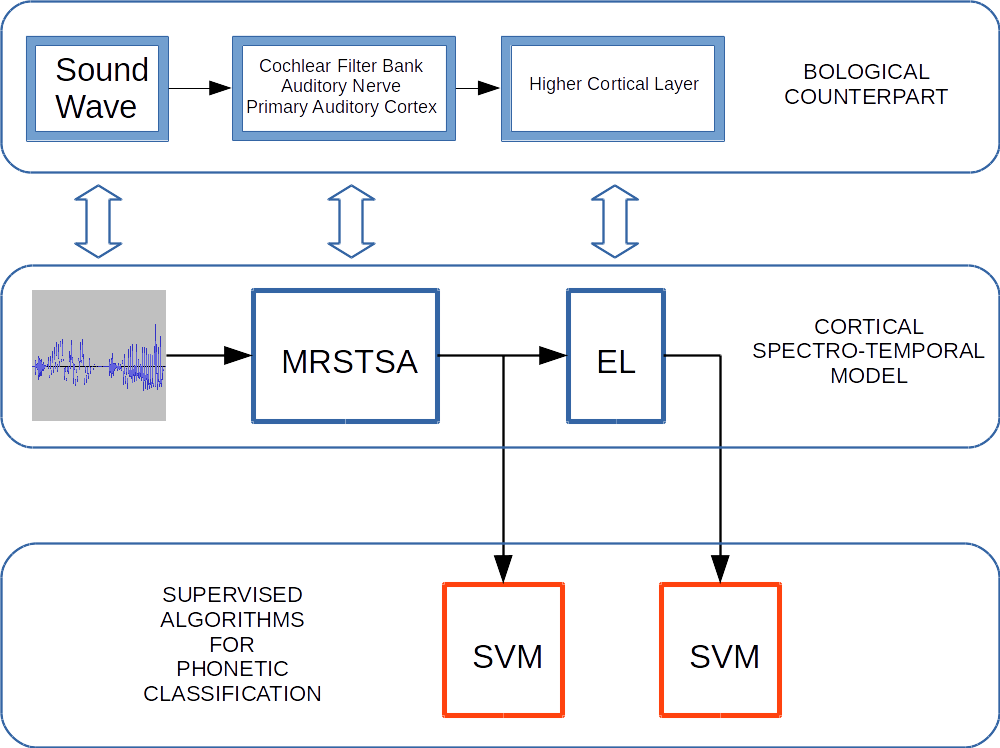
\includegraphics[width=0.8\textwidth]{Experiment.png}
    \caption{Perfil experimental para probar el desempeño en las tareas de clasificación de palabras.
	    Las ondas de sonido son procesadas por el algoritmo \gls{mrstsa}.
    Las salidas desde el \gls{mrstsa} son procesadas por la \gls{el}.
    Las tareas de clasificación de palabras se realizan en ambas salidas por el algpritmo \gls{svm}.
    Cada sección in el \gls{cstm} tiene su contrapartida biológica.}
    \label{fig:Experiment}
\end{figure}

En el procedimiento experimental, primero entrenamos las diferentes \glspl{el}--sección \nameref{model-implementation}--para cada condición silábica. Las \glspl{el}  fueron entrenadas utilizando las voces en el primer conjunto y los corpus generados por medio de los métodos descriptos en la sección \nameref{CorpGen}. Luego, procesamos los mismos corpus con las \glspl{el} correspondientes en modo de inferencia. In tal modo, las \glspl{el} procesaron la información con sus propiedades de aprendizaje deshabilitadas. De esta forma, durante la inferencia, las \glspl{el} no modificaron sus sinapsis y sólo retornaron patrones de activación en respuesta a los estímulos recibidos. Luego, utilizamos las salidas desde el \gls{mrstsa} y desde las \glspl{el} en modo de inferencia para entrenar los clasificadores \gls{svm} con el procedimiento explicado en la sección \nameref{model-implementation}. Los desempeños de entrenamiento promedio de validación cruzada se muestran en Cuadro~\ref{SVM_Training}.

\begin{table}[h!]
\centering
\caption{Resultados para las \glspl{svm} con 5-desdobles y validación cruzada}
\begin{tabular}{|l|l|l|}
\hline
		   & MRSTSA & Encoder Layer \\ \hline
Monosyllabic Words & 99.4\% & 99.52\%          \\ \hline
Disyllabic Words   & 99.3\%   & 99.48\%        \\ \hline
Trisyllabic Words  & 99.5\% & 99.58\%          \\ \hline
\end{tabular}
\label{SVM_Training}
\end{table}

En una segunda etapa, corrimos las \glspl{el} en modo de inferencia, pero esta vez utilizamos corpus diferentes generados utilizando las mismas voces y manipulados con varios tipos de variantes acústicas (ruido blanco, reverberación y variaciones de tono), inyectadas utilizando el software Audacity. También corrimos las \glspl{el} en modo de inferencia utilizando corpus generados con otras voces (del segundo conjunto de voces en la sección \nameref{CorpGen}). Testeamos los desempeños de los clasificadores--ya entrenados--frente a las características devueltas por los algoritmos en respuesta a los corpus afectados por las variantes acústicas que introdujimos en los nuevos corpus utilizando Audacity \cite{audacity}. Las variantes acústicas introducidas en los nuevos corpus incluyeron ruido blanco, reverberación y variaciones de tono. También probamos los desempeños de clasificación frente a las características devueltas por los algoritmos en respuesta a los nuevos corpus generados con un conjunto de voces diferentes.
}{
\subsection{Experiments}

In the present work, we studied the level of invariance in the phonetic features abstracted by the \gls{el}, by means of comparing such representations with the multiresolution spectro-temporal auditory features returned by the \gls{mrstsa} algorithm. To this end, we evaluated the features returned by each algorithm in different word classification tasks. In order to asses word classification performance in each algorithm, we used the \gls{svm} technique--section \nameref{model-implementation}--with  the experimental setup depicted in Fig. \ref{fig:Experiment}.

\begin{figure}[h!]
    \centering
    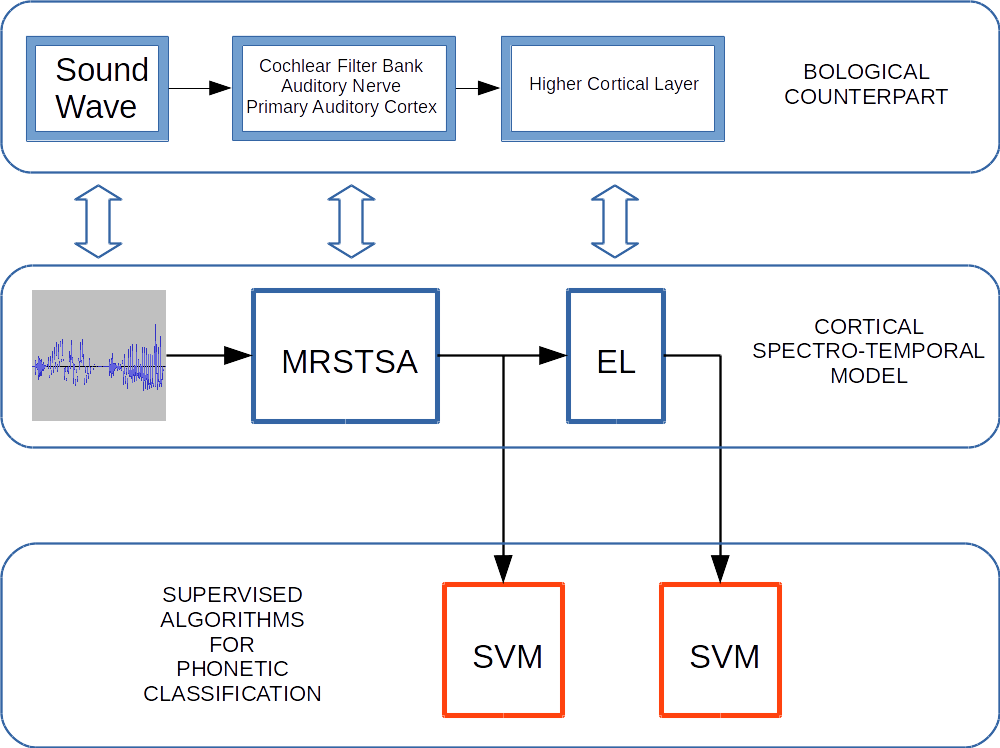
\includegraphics[width=0.8\textwidth]{Experiment.png}
    \caption{Experimental setup to test word classification task performances.
    Sound waves are processed by the \gls{mrstsa} algorithm.
    The outputs from the \gls{mrstsa} are processed by the \gls{el}.
    Word classification tasks are performed on both outputs by the \gls{svm} algorithm.
    Each section in the \gls{cstm} has its biological counterpart.}
    \label{fig:Experiment}
\end{figure}

In the experimental procedure we first trained 10 different \glspl{el}--section \nameref{model-implementation}--for each syllabic condition. Such \glspl{el} were trained using the voices in set one and the corpora were generated by the method described in section \nameref{CorpGen}. Afterwards, we processed the same corpora with the corresponding \glspl{el} in inference mode. In such mode, the \glspl{el} processed the information with their learning properties disabled. In this manner, during inference, the \glspl{el} did not modify its synapses and just returned patterns of activation in response to the stimuli they received. We then used the outputs from the \gls{mrstsa} and the \glspl{el} in inference mode to train the \gls{svm} classifiers with the procedure depicted in section \nameref{model-implementation}. The average cross validation training performances are shown in Table~\ref{SVM_Training}.

\begin{table}[h!]
\centering
\caption{\gls{svm} 5-fold cross validation training results}
\begin{tabular}{|l|l|l|}
\hline
		   & MRSTSA & Encoder Layer \\ \hline
Monosyllabic Words & 99.4\% & 99.52\%          \\ \hline
Disyllabic Words   & 99.3\%   & 99.48\%        \\ \hline
Trisyllabic Words  & 99.5\% & 99.58\%          \\ \hline
\end{tabular}
\label{SVM_Training}
\end{table}

In a second stage, we ran the \glspl{el} in inference mode again, but this time we used different corpora generated using the same voices and manipulated with several types of acoustic variants (white noise, reverberation and pitch variations), generated using the Audacity software. We also ran the \glspl{el} in inference mode using corpora generated with different voices (set two voices in section \nameref{CorpGen}). We tested the performances of the--already trained--classifiers in the presence of the features returned by the algorithms in response to the corpora affected by the acoustic variants which we introduced to the new corpora by means of Audacity \cite{audacity}. The acoustic variants introduced to the new corpora included white noise, reverberation and pitch variations. We also tested the classifier performances in the presence of the features returned by the algorithms in response to the new corpora generated with a different set of voices.
}


























\iftoggle{DEBUG}{
\section{Resultados}

Los desempeños de clasificación se muestran en la Fig. \ref{fig:PLOT}. 

\begin{figure}[h!]
    \centering
    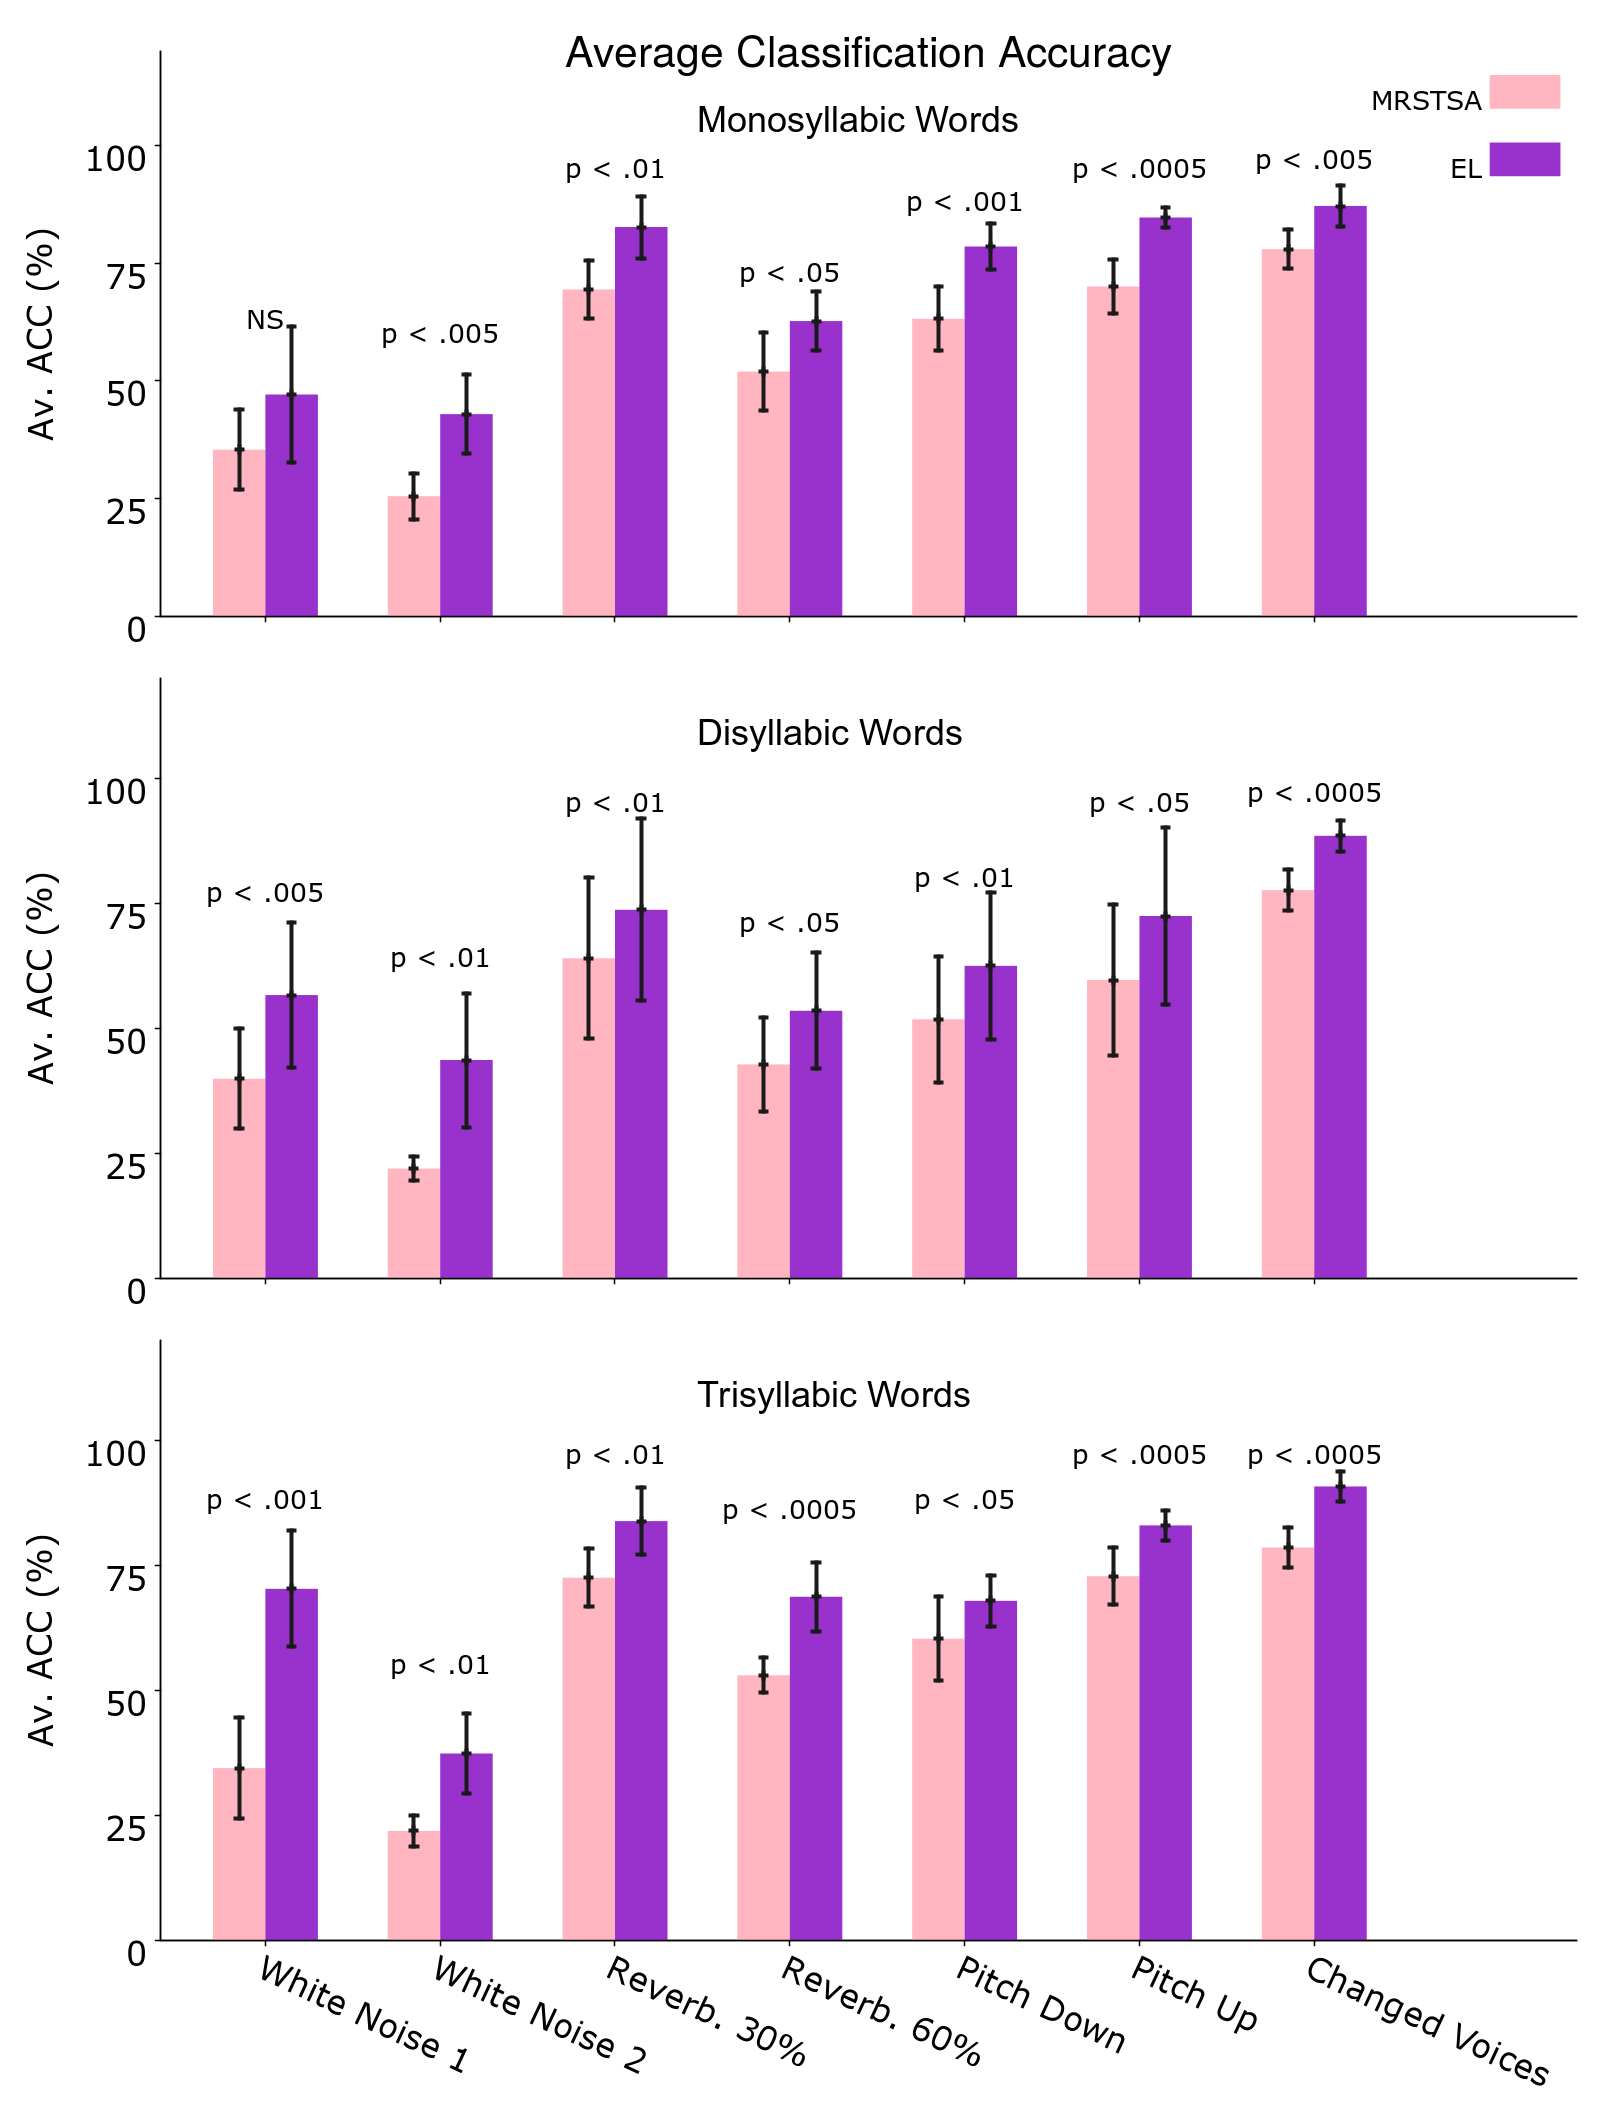
\includegraphics[width=0.8\textwidth]{PLOT.png}
    \caption{Exactitud promedio de clasificación en el \gls{mrstsa} y la \gls{el} frente a diferentes variantes acústicas introducidas en las señales para palabras monosilábicas, bisilábicas y tri-silábicas.
	    Ruido Blanco 1 determina una \glsfirst{snr} de tasa de potencia \gls{rms} promedio de 19.8 dB mientras que Ruido Blanco 2 es de 13.8 dB.
	    Reverberación 30\% determina un valor de \gls{rt} de 0.61 segundos mientras que Reverberación 60\% determina un valor de \gls{rt} de 1.78 segundos.
	    Tono Hacia Arriba determina una corrida de tono desde E hasta G, mientras que Tono Hacia Abajo determina una corrida de tono desde E hasta C. Voces Cambiadas corresponden a los corpus generados utilizando voces diferentes a las voces usadas para entrenar la \gls{el} y los clasificadores. Las barras de error muestran Intervalos de Confianza del 95\%. Los valores de \emph{p} corresponden a t-tests pareados de doble cola y NS indica Estadísticamente no Significativo.}
    \label{fig:PLOT}
\end{figure}

En cuanto al ruido blanco, introducimos ruido blanco aditivo en las señales de los corpus con con una relación de señal a ruido \gls{rms} promedio de tasa de potencia de 19.9 dB (Ruido Blanco 1) y 13.8 dB (Ruido Blanco 2). En cuanto a la reverberación, modificamos las señales de los corpus por medio de valores de \gls{rt} de 0.61 segundos (Reverberación 30\%) y 1.78 segundos (Reverberación 60\%). \gls{rt} hace referencia al tiempo que toma una señal en disminuir su amplitud en 60 dBs por debajo de su valor inicial. En cuanto a las variaciones de tono, modificamos los tonos de las señales en los corpus en +20\% (de E a G) (Tono Hacia Arriba) y en -20\% (de E a C) (Tono Hacia Abajo). También utilizamos corpus generados con voces diferentes a las utilizadas para entrenar las \glspl{el} y las \glspl{svm}.

La Fig. \ref{fig:PLOT} muestra la exactitud en clasificación de 5 vías para corpus de palabras monosilábicas, bisilábicas y tri-silábicas afectadas por ruido blanco, reverberación y variaciones de tono y voz. Como se puede apreciar en las figuras, la \gls{el} supera al \gls{mrstsa} en todos los casos. Tal comportamiento persiste aún en palabras multisilábicas.

Aplicamos t-tests pareados de doble cola para los 10 corpus diferentes generados con los 10 vocabularios diferentes--sección \nameref{CorpGen}. Como se puede ver en la Fig. \ref{fig:PLOT}--exepto para palabras monosilábicas con Ruido Blanco 1 $(p < 0.22)$--obtuvimos significación estadística para todas las condiciones considerando $(p<0.05)$. 
Dado que se llevaron a cabo 7 t-tests para cada tarea de clasificación de palabras independiente (por ejemplo, palabras monosilábicas, bisilábicas y tri-silábicas), aplicamos la corrección de Holm-Bonferroni con un factor de 7 a los fines de reducir la probabilidad de errores de tipo I y de tipo II en el contexto de las diferentes condiciones experimentales \cite{10.1093/biomet/75.2.383}. Por medio de tales correcciones confirmamos la significación estadística para todos los casos mostrados en la Fig. \ref{fig:PLOT}.

La Fig. \ref{fig:PLOT1} muestra la exactitud de clasificación promedio para todas las variantes acusticas para palabras mono, bi y tri-silábicas.
En este caso, también realizamos t-tests pareados de doble cola, pero esta vez para las 7 condiciones de variantes acústicas diferentes.
Como se puede apreciar en la figura, todas la pruebas realizadas fueron estadísticamente significativas  y la capa del Encoder muestra una clara superioridad que se sostiene para palabras diferente número de sílabas.

\begin{figure}[h!]
    \centering
    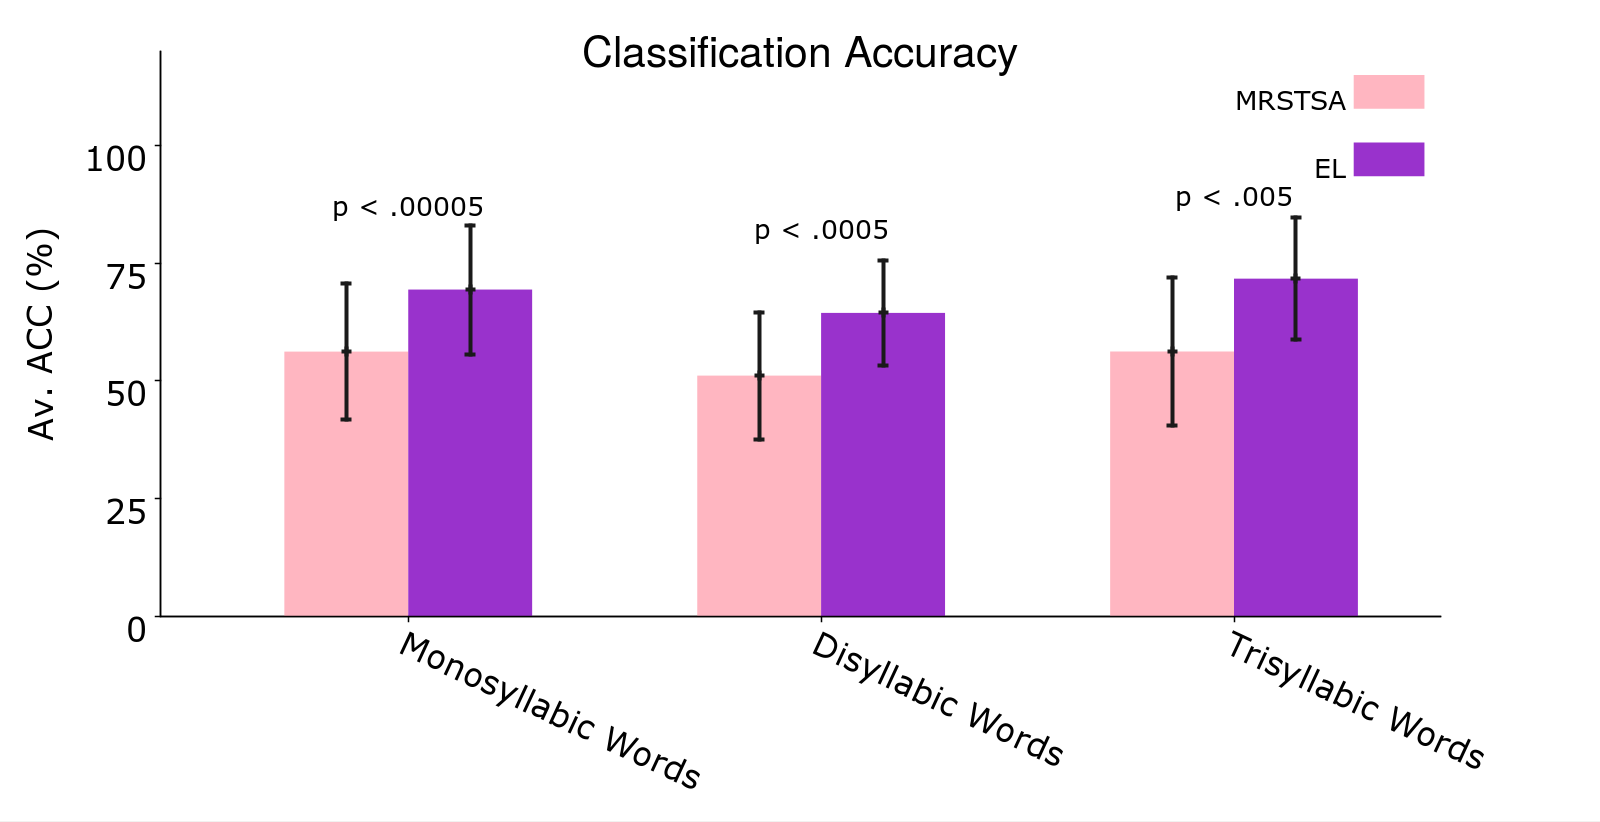
\includegraphics[width=0.8\textwidth]{PLOT1.png}
    \caption{Exactitud en clasificación promedio a través de todas las variantes acústicas para palabras mono, bi y trisilábicas. Las barras de error exhiben un Intérvalo de Confianza del 95\%. Los valores de \emph{p} corresponden a t-tests pareados de doble cola.}
    \label{fig:PLOT1}
\end{figure}
}{
\section{Results}

The classification performances are shown in Fig. \ref{fig:PLOT}.

\begin{figure}[h!]
    \centering
    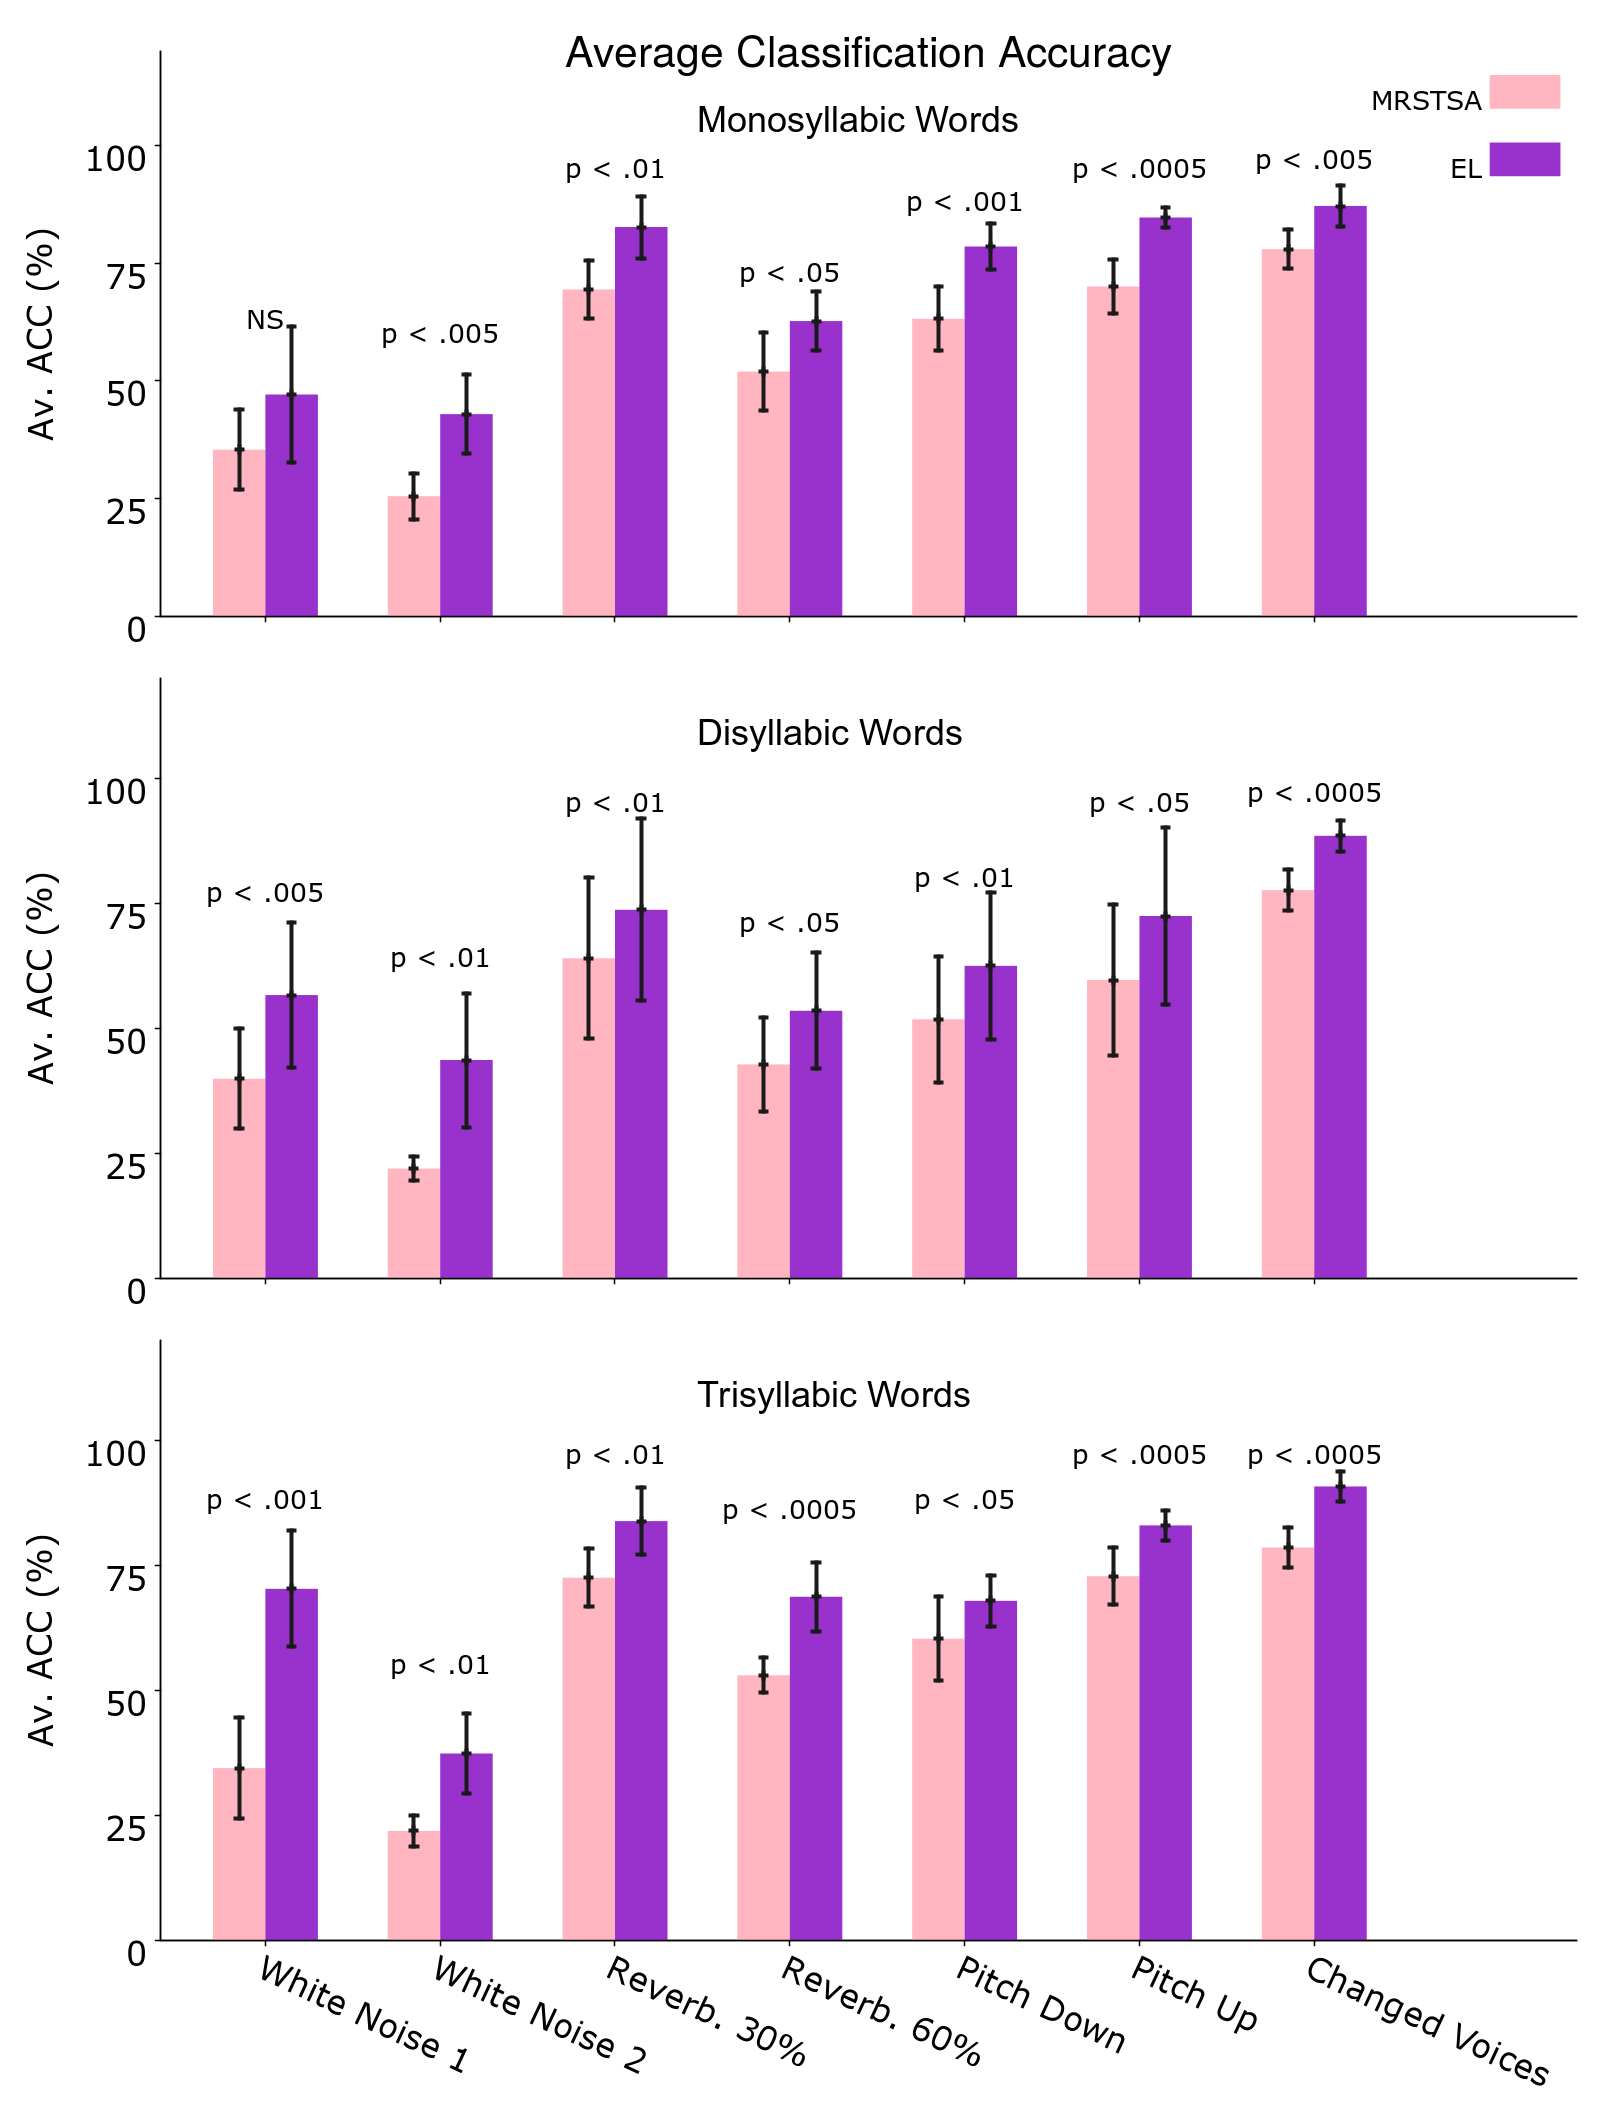
\includegraphics[width=0.8\textwidth]{PLOT.png}
    \caption{\gls{mrstsa} and \gls{el} average classification accuracies against different acoustic variants introduced to the signals
    for monosyllabic, disyllabic and trisyllabic words.
    White Noise 1 determines a \gls{snr} average \gls{rms} power rate of 19.8 dB while White Noise 2 13.8 dB.
    Reverberation 30\% determines a \gls{rt} value of 0.61 seconds while Reverberation 60\% determines a \gls{rt} value of 1.78 seconds.
    Pitch Up determines a pitch move from E to G, while Pitch Down determines a pitch move from E to C. Changed Voices corresponds to corpora generated using a different set of voices from the one used to train the \glspl{el} and the classifiers. Error bars depict 95\% Confidence Interval values. The \emph{p} values correspond to two-tailed} paired t-tests and NS stands for Not Statistically Significant.
    \label{fig:PLOT}
\end{figure}

Regarding white noise, we introduced additive white noise to the corpora signals with signal-noise average \gls{rms} power rate of 19.9 dB (White Noise 1) and 13.8 dB (White Noise 2). In terms of reverberation, we modified the corpora signals by means of \gls{rt} values of 0.61 seconds (Reverberation 30\%) and 1.78 seconds (Reverberation 60\%). \gls{rt} Is the time that a signal takes to decrease its amplitude to 60 dBs under its initial value. As regards pitch variations, we modified the corpora signals pitch in +20\% (from E to G) (Pitch Up) and in--20\% (from E to C) (Pitch Down). We also used corpora generated with different voices from the ones used to train the \glspl{el} and the \glspl{svm}.

Fig. \ref{fig:PLOT}
shows a 5-way word classification accuracy for mono, di and trisyllabic word corpora affected by
white noise, reverberation and pitch and voice variations.
As can be seen in the figures, the \gls{el} outperforms the \gls{mrstsa} in all cases.
Such behavior persists for multisyllabic words.

We performed two-tailed paired t-tests for 10 different corpora generated from 10 different vocabularies--section \nameref{CorpGen}. As can be seen in Fig. \ref{fig:PLOT}--except for monosyllabic words with White Noise 1 $(p < 0.22)$--there was Statistical Significance for all conditions considering $(p<0.05)$.

Given that we conducted 7 t-tests for each independent word classification task (i.e. mono, di and trisyllabic words), we performed Holm–Bonferroni corrections with a correction factor of 7 in order to reduce the probability of type I and type II errors in the context of the different experimental conditions \cite{10.1093/biomet/75.2.383}. By means of such corrections we confirmed the statistical significance for all the cases showed in Fig.\ref{fig:PLOT}.

Fig. \ref{fig:AV_ACC} shows average classification accuracies across all acoustic variants for mono, di and trisyllabic words.
In this case, we also performed two-tailed paired t-tests, but this time for 7 different acoustic variant conditions.
As can be seen in the figure, all performed tests are statistically significant and the encoder layer clearly shows
a sustained superiority across words with different number of syllables.

\begin{figure}[h!]
    \centering
    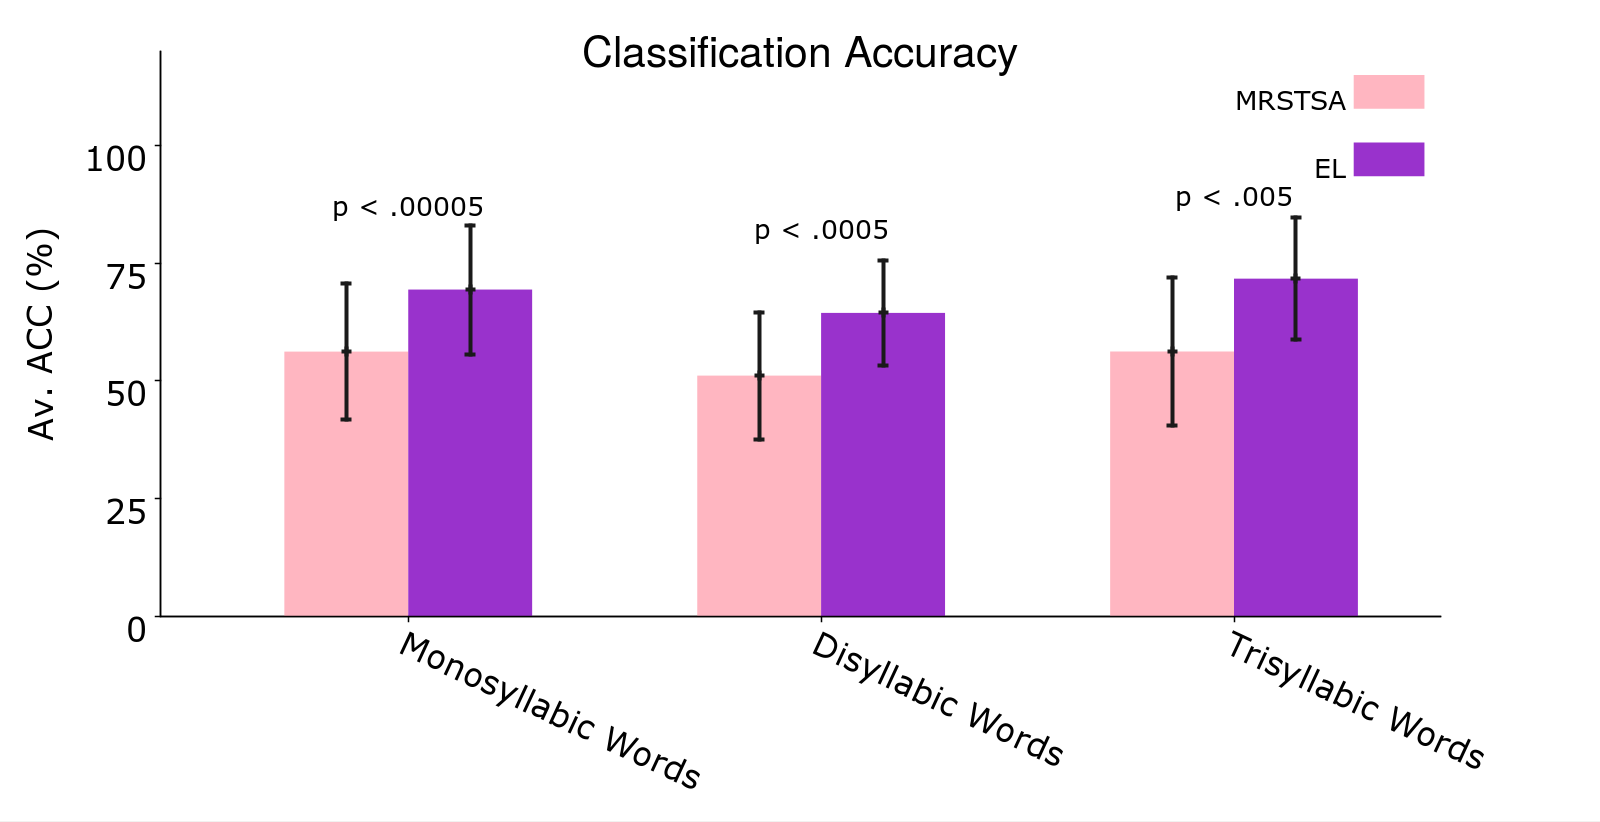
\includegraphics[width=0.8\textwidth]{PLOT1.png}
    \caption{Average classification accuracies across all acoustic variants for mono, di and trisyllabic words. Error bars depict 95\% Confidence Interval values. The \emph{p} values correspond to two-tailed paired t-tests}.
    \label{fig:AV_ACC}
\end{figure}
}

















\iftoggle{DEBUG}{
\section{Discusión}

Los resultados obtenidos en este trabajo sostienen las hipótesis computacionales propuestas en nuestro enfoque de modelaje para imitar la invarianza y la generalización fonética incidental.
Algunas de las hipótesis ya han sido explicadas en términos de sus propiedades  \cite{hawkins_2016}, pero más específicamente en términos de sus capacidad de aprendizaje de secuencias \cite{cui_2016}.
De todas maneras, no existen precedentes de tales características neurofisiológicas probadas en tareas de clasificación como las que se llevan acabo en el presente trabajo, en las que las reglas fonotácticas se adquieren sin la aplicación de procedimientos de obtimización como retro-propagando errores por medio de \emph{descenso de gradiente}. Adicionalmente, nuestro enfoque presenta diferencias sustanciales en términos de sus características de implementación algorítmica. En este trabajo, las sinapsis distales proveen contribuciones individuales de valores continuos y nuestra organización anatómica micro-columnar adquiere su comportamiento fisiológico espontaneamente con el aprendizaje. También probamos tales características en una realización con cientos de columnas corticales cada una combinando varias micro-columnas con activaciones aferentes estocásticas cuyas implementaciones futuras estás destinadas a explorar simulaciones a gran escala en sistemas computacionales de alto desempeño.

Algunos modelos computacionales han sido desarrollados previamente para entender como las categorías fonéticas son adquisidas~\cite{rasanen_2012}. El objetivo en dichos trabajos ha sido principalmente explicar aspectos relevantes de la adquisición fonética, sin dar detalles en cuanto a cómo el cerebro podría proveer tales computaciones.
Lee et al. (2009), empleó aprendizaje no supervisado para clasificación de audio con \gls{cdbn_pl}~\cite{Lee:2009:UFL:2984093.2984217}. 
Los autores probaron el desempeño en clasificación de un modelo con dos capas en la exactitud de una tarea de clasificación de fonemas en 39 vías sobre el conjunto de datos \gls{timit} para varios números de oraciones de entrenamiento. 
La primera capa nunca superó el algoritmo de \gls{mfcc} que fue utilizado como entrada a la red.
Es más, en tal trabajo no se reportó el desempeño de la segunda capa ya que esta no pudo superar a la primera.
El máximo desempeño reportado para la primer capa fue del 64.4\% contra un desempeño del 79.6\% para el \gls{mfcc}.
Sólo fue posible reportar un desempeño del 80.3\% combinando ambos, el \gls{mfcc} y la primer capa en la \gls{cdbn}.

En un trabajo más reciente, la capacidad de \glspl{dmn}--una modificación de arquitectura de \glspl{dnn} alimentada en directo que utiliza la función de activación max-out--para manejar ruido ambiental fue investigada frente a diferentes clases fonéticas y para diferentes condiciones de ruido \cite{silos_2016}. En tales experimentos--con la excepción de fonemas fricativos para 15 dB \gls{snr} de Ruido Callejero--el desempeño nunca superó el 70\%. De hecho, el desempeño se vio seriamente deteriorado en presencia de ruido blanco de 15 dB \gls{snr}, resultando en una exactitud de clasificación bien por debajo del 60\% en todos los casos.

En el trabajo aquí presentado, reportamos desempeños en clasificación de--por ejemplo--90.8\% para la \gls{el} contra 78.58\% para el \gls{mrstsa} para palabras trisilábicas frente a voces cambiadas (es decir, voces que nunca fueron \emph{oidas} por la \gls{el} durante el entrenamiento; Fig. \ref{fig:PLOT}), también reportamos desempeños por encima del 70\% en la \gls{el} contra un desempeño por debajo del 35\% en el \gls{mrstsa} para palabras trisilábicas frente a ruido blanco de 19.8dB \gls{snr} y desempeños bien arribade 40\% para palabras mono y bisilábicas frente a ruido blanco de 13.8 dB \gls{snr} (Fig. \ref{fig:PLOT}). También reportamos que la \gls{el} superó al \gls{mrstsa} para todas las condiciones de prueba y que tal comportamiento se sostuvo para diferentes números de sílabas en las palabras utilizando pruebas de significación estadística (Fig. \ref{fig:PLOT1}).

Aunque este es un buen escenario, debemos de ser cuidadosos ya que no podemos ignorar diferencias experimentales importantes con respecto a los resultados arrojados por los trabajos previos. Primero, nuestro material de entrenamiento es muy diferente  al utilizado en dichos trabajos. Nosotros utilizamos corpus generados por sintetizadores de vos en lugar de corpus estandarizados como \gls{timit}.
Nuestro principal objetivo fue el de replicar adquisición fonética temprana en humanos, lo cual es logrado incidentalmente por infantes \cite{Saffran1996StatisticalLB}.
Dada la buena calidad de las voces sintetizadas por \gls{festival}  \cite{festival2014} y su flexibilidad para componer diferentes tipos de corpus--aún con palabras que no existen en ningún lenguaje--consideramos apropiada su utilización como procedimiento experimental inicial para probar nuestro enfoque en un contexto de reglas fonotácticas adquiridas incidentalmente.
Segundo, en este trabajo abordamos tareas de clasificación de palabras multililábicas en contraste con los experimentos de clasificación de fonemas llevados a cabo por las investigaciones previas, ya que estamos principalmente motivados por probar las capacidades de la dinámica secuencial de nuestro modelo para adquirir las reglas fonotácticas que subyacen los vocabularios de entrenamiento.
Finalmente, reportamos resultados de tareas de clasificación de 5 vías en contraste con tareas de clasificación de 39 vías en \cite{Lee:2009:UFL:2984093.2984217}.
Por un lado, esta última diferencia podría haber actuado en favor de nuestro enfoque considerando que es más facil clasificar una categoría entre 5 que una entre 39.
Por otro lado, es importante resaltar que los trabajos previos han estado provistos de más material de entrenamiento con más vocabularios, más hablantes, etc.
En nuestro caso, presentamos condiciones de entrenamiento más duras, ya que nuestro modelo fue entrenado con 500 palabras desde un vocabulario de solo 5 palabras pronunciadas por 10 voces.
Más allá del tamaño pequeño de la muestra, el desempeño demostrado por nuestro modelo computacional exhibe niveles significativos de generalización fonética con la capacidad de adquirir reglas fonotácticas y de generalizar a contextos ambientales novedosos. El nuestro es un escenario mucho más biológicammente preciso que aquellos establecidos por otros enfoques en los cuales sus modelos son entrenados utilizando millones de ejemplos. Nuestro modelo, por lo tanto, imita resultados experimentales que muestran como infantes de 8 meses de edad adquieren las reglas fonotácticas inmersas el el flujo auditivo de entrada con sólo 2 minutos de exposición (180 palabras en total, de un vocabulario de 4 palabras de tres sílabas) \cite{Saffran1996StatisticalLB}.

Somos conscientes que se necesitarán mas pruebas--en diferentes escenarios--con corpus diferentes y estandardizados (como \gls{timit}) para analizar más profundamente las capacidades de nuestro enfoque.
Sin embargo, nuestro objetivo principal en el presente trabajo fue el de probar la invarianza fonética secuencial exhibida por la \gls{el} bajo condiciones experimentales estrictamente controladas en las que se conocieron los niveles de ruido, reverberación y variaciones de tono con los que el estímulo se afectó de manera precisa. El material de entrenamiento para la \gls{el} solo involucró los corpus originales de 500 palabras, pero lo más importante es que la \gls{el} nunca fue expuesto--durante su entrenamiento--a los disturbios utilizados para probar el desempeño de su clasificación. El perfil experimental aplicado en este trabajo (Fig. \ref{fig:Experiment}) deja en claro que la \gls{el} es íntegramente no supervisado y que toda la supervisión se limita a los algoritmos de \gls{svm}. Más aún, la \gls{el} no optimiza la actualización de sus pesos sinápticos utilizando descenso del gradiente retro-propagando errores producidos por funciones de costo arbitrariamente insertadas. Este es un punto fundamental para demostrar la plausibilidad biológica de nuestra implementación ya que las restricciones fonotácticas en los  lenguajes humanos son adquiridas incidentalmente \cite{BRENT199693,saffran_1997} y por lo tanto, supervisión alguna podría ser tolerada bajo tales circunstancias comportamentales.

En futuras investigaciones ciertas propiedades dinámicas emergentes podrían surgir de la incorpoaración de capas corticales subsecuentes--más allá de la \glsfirst{el}--en los pasos de procesamiento del modelo. De esta forma podremos implementar dendritas apicales distales hacia atrás las cuales traerán contexto por medio de una implementación jerárquica no supervisada.
Aunque tal retroalimentación podría ser útil en el contexto de la adquisición fonética incidental, el modelado de la competencia fonética adulta podría requerir la implementación de hipótesis más complejas para nuestro modelo. La incorporación de funciones de costo con más precisión biológica para poder retroalimentar cualquier tipo de error de activación requerirá hipótesis biológicamente precisas. ¿Deberían esos errores ser señales escalares (mecanismos de refuerzo) o deberían ser vectores (mecanismos supervisados)? ¿Deberían de venir desde la misma modalidad o deberían ser traídas desde una modalidad diferente? ¿Deberían variar a través de parches corticales diferentes o deberían variar durante el desarrollo temporal? \cite{10.3389/fncom.2016.00094}.
Un mecanismo supervisado asistido por diferentes áreas corticales de forma multimodal podría ser una hipótesis biológicamente precisa ya que se ha mostrado como gestos icónicos impulsan la comprensión del habla bajo condiciones auditivas adversas \cite{HOLLE2010875}.
Incluso, la conectividad funcional a través de diferentes áreas corticales facilita la comprensión del habla cuando la inteligibilidad de la señal es reducida~\cite{Obleser2283}. Sin embargo, más allá de hipótesis en relación a funciones de costo, también es importante determinar los algoritmos utilizados para retroalimentar errores de activación. Independientemente del hecho de que el método de descenso de gradiente es--a primera vista--demasiado complejo para ser implementado por el tejido cortical, varios estudios sostienen la idea de que la asignación de crédito--el objetivo último en backpropagation--podría ser un fenómeno presente en el cerebro \cite{Guerguiev2017TowardsDL}. De hecho, en \cite{Lillicrap_2016} los autores presentan un mecanismo que realiza backpropagation relajando la arquitectura de conectividad en reverso y asignando culpa multiplicando errores por pesos sinapticos aleatorios.
Más allá de todo lo arriba mensionado, no existe prueba de que el cerebro implemente descenso de gradiente de la manera en que se implementa en redes \glspl{dnn} actuales, por lo tanto, nuevas estrategias--con más plausibilidad biológica--podrían surgir desde la comunidad científica en el futuro.

En versiones futuras del modelo se aumentará su plausibilidad biológica incrementando el número de células por \gls{cc} con simulaciones en sistemas \gls{hpc} de escalado masivo y utilizando un \gls{gsom} por \gls{cc} a los fines de incorporar reclutamiento de recursos neuronales en cada \gls{cc} dependiendo de la dispersión estadística del estímulo \cite{Meyer19113}. Por ejemplo, un arreglo tetradimensional de unidades neuronales se podría emplear para simular columnas corticales de aproximadamente 34.000 células. De esta manera, miles de columnas corticales se podrían organizar en arreglos multidimensionales. A través de la utilización de supercomputadoras de clase lider (por ejemplo, recursos posicionados en la lista del Top 500 en computación, \url{top500.org}), y asumiendo una columna cortical por nodo computacional con 64 núcleos, correríamos aproximadamente 256.000 hilos. Tales simulaciones nos permitirían elevar la capacidades de adquisición así como generalización fonética considerablemente más allá de los niveles reportados en este trabajo.
}{
\section{Discussion}

Results obtained in the present work support the computational hypotheses posed in our modeling approach in order to mimic incidental phonetic invariance and generalization.
Some of these hypotheses have already been explained in terms of their properties \cite{hawkins_2016}, but more specifically in terms of their sequence learning capabilities \cite{cui_2016}.
Nevertheless, there are no precedents of such neurophysiological features tested in word classification tasks as the ones carried out here, in which phonotactic rules are acquired without the application of optimization procedures such as backpropagating errors by means of gradient descent. In addition, our approach presents substantial differences in terms of feature algorithmic implementation. In the present work, distal synapses make continuous individual contributions and our anatomical micro-columnar organization acquires its physiological behavior spontaneously from learning. We also tested such features in a realization with hundreds of cortical columns each combining several micro-columns with stochastic afferent activation whose future implementations are intended to explode large-scale simulations in leadership supercomputers.

Computational models have been previously developed to understand how phonetic categories are acquired~\cite{rasanen_2012}. The goal in these works has been mainly to explain relevant aspects of phonetic acquisition, without details about how the brain might provide such computations. 
Lee et al. (2009), employed unsupervised feature learning for audio classification with \glspl{cdbn}~\cite{Lee:2009:UFL:2984093.2984217}.
The authors tested classification performance of a model with two layers in a 39-way phone classification accuracy task on the test data \gls{timit} for various numbers of training sentences.
The first layer never outperformed the \gls{mfcc} algorithm that was used as input for the network.
Furthermore, such work did not report the second layer performance since it could not outperform the first one.
The maximum performance reported for the first layer was 64.4\% vs. a performance of 79.6\% for the \gls{mfcc}.
It was just possible to report a performance of 80.3\% by means of combining both, the \gls{mfcc} and the first layer in the \gls{cdbn}.

In a more recent work, the capacity of \glspl{dmn}--a modification of \glspl{dnn} feed-forward architecture that uses a max-out activation function--to handle environmental noise was investigated into different broad phonetic classes and for different noise conditions \cite{silos_2016}.  In such experiments--with the exception of fricatives phonemes for 15 dB \gls{snr} Street Noise--accuracy never exceeded 70\%. Furthermore, performance was seriously impaired in the presence of 15 dB \gls{snr} white noise, resulting in classification accuracy  well below 60\% in all cases.

In the present work, we reported classification performances of--for example--90.8\% on the \gls{el} vs. 78.58\% on the \gls{mrstsa} for trisyllabic words against Changed Voices (i.e. voices never ``heard'' by the \gls{el} during training; Fig. \ref{fig:PLOT}), we also reported a performance above 70\% on the \gls{el} vs. a performance below 35\% on the \gls{mrstsa} for trisyllabic words against 19.8 dB \gls{snr} white noise and performances well above 40\% for mono and disyllabic words against 13.8 dB \gls{snr} white noise (Fig. \ref{fig:PLOT}). We also reported that the \gls{el} outperformed the \gls{mrstsa} for all the test conditions and that this behavior was sustained through different number of syllables in the words by means of statistical significance tests (Fig. \ref{fig:AV_ACC}).

Although this is a compelling scenario, we have to be cautious since we cannot ignore important experimental differences from previous research results. First, our training material was very different from that found in previous works. We used corpora generated by synthesized voices instead of standardized \gls{timit} corpora.
Our main aim was to mimic early phonetic acquisition in humans, which is incidentally accomplished by infants \cite{Saffran1996StatisticalLB}.
Given the high quality of the voices synthesized by \gls{festival} \cite{festival2014} and its flexibility in order to compose different kind of corpora--even with words that do not exist in any language--we considered that this was an appropriate initial experimental procedure to test our approach in a context of incidentally acquired phonotactic rules. 
Second, we pursued multisyllabic words classification tasks in contrast to the phone classification experiments carried out in previous research,
since we mainly aimed to test the dynamic sequential capability of our model to acquire the phonotactic rules behind the training vocabularies. 
Finally, we reported results on 5-way classification tasks vs. performance on 39-way classification tasks in \cite{Lee:2009:UFL:2984093.2984217}. 
On the one hand, this last difference may have acted in favour of our approach considering that it is easier to classify one category among 5 than one among 39.
On the other hand, it is important to highlight that previous works have had more extended training material with more vocabularies, more speakers, etc.
In our case, we presented more difficult training conditions, since our model was trained with 500 words from a vocabulary of just 5 words uttered by 10 voices.
Despite the small sample size, the performance obtained by our neurocomputational model exhibits a significant level of phonetic generalization with the capacity to acquire phonotactic rules and to generalize to novel environmental contexts. This is a much more biologically accurate scenario than those settled by other approaches, in which models are trained using millions of examples. Our model therefore mimics experimental results which show that 8-month-old infants  acquire the phonotactic rules immersed in auditory input streams with only 2 minutes of exposure (180 words in total, from a vocabulary of four three-syllable words) \cite{Saffran1996StatisticalLB}.

We are aware that more tests--in different scenarios--with different and standardized corpora (such as \gls{timit}) will be needed to analyze the capacities of our approach more deeply.
Nevertheless, our main objective in the present work was to assess the sequential phonetic invariance exhibited by the \gls{el} under strictly controlled experimental conditions in which we precisely knew the levels of noise, reverberation and pitch variations with which the stimulus was affected. The \gls{el} training material included only the original corpora with 500 words, but more importantly, the \gls{el} was never exposed--during learning--to the disturbances used to test its classification performance. The experimental profile applied in this work (Fig. \ref{fig:Experiment}) makes it clear that the \gls{el} is completely unsupervised and that all supervision is limited to the \gls{svm} algorithm. Furthermore, the \gls{el} does not optimize its synaptic weight updates using gradient descent backpropagating errors from arbitrarily inserted loss functions. This is a fundamental point to demonstrate the biological plausibility of our implementation since phonotactic constraints in a human language are learned incidentally \cite{BRENT199693,saffran_1997} and therefore, no supervision could be supported under such behavioral circumstances. 

In future researches, emergent dynamic properties could arise from the addition of subsequent cortical layers--beyond the \glsfirst{el}--in the processing pipeline of this model.  In this way we will be able to implement backward distal apical dendrites, which will bring context through an unsupervised hierarchical implementation. Even though such feedback could be beneficial in an incidental phonetic acquisition context, modeling adult phonetic competence could possibly require the implementation of more complex hypotheses in our model. The incorporation of biologically accurate cost functions in order to feed back any kind of activation error would require precise biological hypotheses. Should those errors be scalar signals (reinforcement mechanisms) or should they be vectors (supervised mechanisms)? Should they come from the same modality or should they be gathered from a different one? Should they vary across different cortical patches or should they vary during temporal development? \cite{10.3389/fncom.2016.00094}. A supervised mechanism assisted from different cortical areas in a multimodal fashion could be a biologically accurate hypothesis, since it has been shown that iconic gestures boost speech comprehension under adverse listening conditions \cite{HOLLE2010875}. Furthermore, functional connectivity across different cortical areas facilitates speech comprehension when the intelligibility of the speech signal is reduced~\cite{Obleser2283}. Yet, beyond the cost functions hypotheses, it is also important to determine the algorithms used to feed back activation errors. Regardless of the fact that gradient descent is--at first glance--too complex to be implemented by cortical tissue, several studies support the idea that credit assignment--the ultimate goal of backpropagation--could be a phenomenon present in the brain \cite{Guerguiev2017TowardsDL}. Furthermore, in \cite{Lillicrap_2016} the authors presented a mechanism that performs backpropagation relaxing the backward connectivity architecture and assigning blame by multiplying errors by random synaptic weights. Apart from the above, there is no proof that the brain implements gradient descent as it is implemented in current \glspl{dnn}, thus novel strategies--with more biological plausibility--could arise from the scientific community in the future.

Future versions of the model will increase biological plausibility by increasing the number of cells per \gls{cc} with massively scaling \gls{hpc} simulations and using a \gls{gsom} per \gls{cc} in order to incorporate neural resource recruitment specialization in each \gls{cc} depending on the statistical dispersion of its stimuli \cite{Meyer19113}. For instance, a four-dimensional array of neural units can be employed to simulate cortical columns of approximately 34,000 cells. In this way, thousands of cortical columns can be organized in multidimensional arrays. Using a leadership-class supercomputer (e.g. resources from the Top 500 computing list, \url{top500.org}), and assuming one cortical column per compute node with 64 cores, we could be running 527 neural units per thread in a CPU. Furthermore, configuring a three-dimensional array of 1000 cortical columns per cortical layer, a model of 4 layers could be running on approximately 256,000 threads. Such simulations could allow us to leverage phonotactic acquisition as well as phonetic generalization capacities beyond the levels reported in this paper.
}



























\iftoggle{DEBUG}{
\section{Conclusiones}

En este trabajo, analizamos representaciones invariantes fonotácticas secuenciales para altos niveles en la via auditiva en respuesta a estímulos de sonidos fonéticos complejos. Investigamos tales representaciones en relación a características potencialmente relevantes de la corteza auditiva. Incorporamos tales características en un modelo computacional--dentro de la etapa \gls{el} en un modelo llamado \gls{cstm}--y utilizamos clasificación por medio de \gls{svm} para probar su desempeño para varias tareas de clasificación de palabras. Comparamos el desempeño de nuestro modelo con el desempeño alcanzado por el algoritmo \gls{mrstsa}. La \gls{el} muestra capacidades de adquisición fonotáctica secuencial prominentes, superando al algoritmo \gls{mrstsa} en todas las pruebas realizadas. Debido a que el perfil experimental está diseñado para probar los niveles de generalización fonética en ambos algoritmos, exponiendo el material de entrenamiento a disturbios ambientales y a variaciones de tono, nuestro modelo muestra capacidad de generalización fonética significativa, mejorando el desempeño del \gls{mrstsa}--aún cuando este ha sido comprometido seriamente. 

En futuras investigaciones, propiedades dinámica emergentes podrían surgir de la adición de capas corticales subsecuentes--más allá del \glsfirst{el}--en las etapas de procesamiento de este modelo. De esta forma podremos implementar dendritas apicales distantes hacia atrás, las cuales traerán contexto por medio de una implementación jerárquica no supervisada. También planeamos incorporar más plausibilidad biológica incrementando el número de células por \gls{cc} por medio de escalamiento masivo en simulaciones de \gls{hpc} y utilizando un \gls{gsom} por \gls{cc} a los fines de incorporar especialización en el reclutamiento de recursos neuronales en cada \gls{cc} dependiendo de la dispersión estadística en sus estímulos \cite{Meyer19113}.

Aunque investigación adicional futura--con más material experimental--será requerida, los hallazgos presentados aquí podrían ser influyentes delineando caminos nuevos y alternativos a las tecnologías actuales de percepción profunda en general y, más específicamente, en términos de características neurofisiológicas específicas relevantes para adquisición temprana de lenguaje por reglas fonotácticas en infantes.
}{
\section{Conclusion}

In this paper, we analyze the sequential phonotactic invariant representations of high levels auditory pathway responses to complex phonetic sound stimuli.  We research such representations in relation to potentially relevant features in the auditory cortex. We incorporate such features in a computational model--inside the \gls{el} stage of a model called \gls{cstm}--and use \gls{svm} classification to test its performance for several word classification tasks. We compare our model performance with the performance achieved by the \gls{mrstsa} algorithm. The \gls{el} shows prominent sequential phonotactic acquisition capabilities, outperforming the \gls{mrstsa} algorithm for all the tests performed. Since the experimental profile is designed to asses the level of phonetic generalization on both algorithms, exposing the training material to environmental and pitch disturbances not present during learning, our model shows significant phonetic generalization capacity, leveraging the performance of the \gls{mrstsa}--even when it is seriously impaired. 

In future research
emergent dynamic properties could arise from the addition of subsequent cortical layers--beyond the \glsfirst{el}--in the processing pipeline of this model.  In this way we will be able to implement backward distal apical dendrites, which will bring context through an unsupervised hierarchical implementation. We are also planning to add more biological plausibility by means of increasing the number of cells per \gls{cc} with massively scaling \gls{hpc} simulations and using a \gls{gsom} per \gls{cc} in order to incorporate neural resource recruitment specialization in each \gls{cc} depending on the statistical dispersion in its stimuli \cite{Meyer19113}.

Although future research with more experimental material will be needed, the research findings presented herein will be influential in terms of drawing new and alternative paths to current deep perception technologies in general and, more specifically, towards specific neurophysiological features plausibly relevant for phonotactic infant language acquisition.

}










